\documentclass[twoside]{book}

% Packages required by doxygen
\usepackage{fixltx2e}
\usepackage{calc}
\usepackage{doxygen}
\usepackage[export]{adjustbox} % also loads graphicx
\usepackage{graphicx}
\usepackage[utf8]{inputenc}
\usepackage{makeidx}
\usepackage{multicol}
\usepackage{multirow}
\PassOptionsToPackage{warn}{textcomp}
\usepackage{textcomp}
\usepackage[nointegrals]{wasysym}
\usepackage[table]{xcolor}

% Font selection
\usepackage[T1]{fontenc}
\usepackage[scaled=.90]{helvet}
\usepackage{courier}
\usepackage{amssymb}
\usepackage{sectsty}
\renewcommand{\familydefault}{\sfdefault}
\allsectionsfont{%
  \fontseries{bc}\selectfont%
  \color{darkgray}%
}
\renewcommand{\DoxyLabelFont}{%
  \fontseries{bc}\selectfont%
  \color{darkgray}%
}
\newcommand{\+}{\discretionary{\mbox{\scriptsize$\hookleftarrow$}}{}{}}

% Page & text layout
\usepackage{geometry}
\geometry{%
  a4paper,%
  top=2.5cm,%
  bottom=2.5cm,%
  left=2.5cm,%
  right=2.5cm%
}
\tolerance=750
\hfuzz=15pt
\hbadness=750
\setlength{\emergencystretch}{15pt}
\setlength{\parindent}{0cm}
\setlength{\parskip}{3ex plus 2ex minus 2ex}
\makeatletter
\renewcommand{\paragraph}{%
  \@startsection{paragraph}{4}{0ex}{-1.0ex}{1.0ex}{%
    \normalfont\normalsize\bfseries\SS@parafont%
  }%
}
\renewcommand{\subparagraph}{%
  \@startsection{subparagraph}{5}{0ex}{-1.0ex}{1.0ex}{%
    \normalfont\normalsize\bfseries\SS@subparafont%
  }%
}
\makeatother

% Headers & footers
\usepackage{fancyhdr}
\pagestyle{fancyplain}
\fancyhead[LE]{\fancyplain{}{\bfseries\thepage}}
\fancyhead[CE]{\fancyplain{}{}}
\fancyhead[RE]{\fancyplain{}{\bfseries\leftmark}}
\fancyhead[LO]{\fancyplain{}{\bfseries\rightmark}}
\fancyhead[CO]{\fancyplain{}{}}
\fancyhead[RO]{\fancyplain{}{\bfseries\thepage}}
\fancyfoot[LE]{\fancyplain{}{}}
\fancyfoot[CE]{\fancyplain{}{}}
\fancyfoot[RE]{\fancyplain{}{\bfseries\scriptsize Generated by Doxygen }}
\fancyfoot[LO]{\fancyplain{}{\bfseries\scriptsize Generated by Doxygen }}
\fancyfoot[CO]{\fancyplain{}{}}
\fancyfoot[RO]{\fancyplain{}{}}
\renewcommand{\footrulewidth}{0.4pt}
\renewcommand{\chaptermark}[1]{%
  \markboth{#1}{}%
}
\renewcommand{\sectionmark}[1]{%
  \markright{\thesection\ #1}%
}

% Indices & bibliography
\usepackage{natbib}
\usepackage[titles]{tocloft}
\setcounter{tocdepth}{3}
\setcounter{secnumdepth}{5}
\makeindex

% Hyperlinks (required, but should be loaded last)
\usepackage{ifpdf}
\ifpdf
  \usepackage[pdftex,pagebackref=true]{hyperref}
\else
  \usepackage[ps2pdf,pagebackref=true]{hyperref}
\fi
\hypersetup{%
  colorlinks=true,%
  linkcolor=blue,%
  citecolor=blue,%
  unicode%
}

% Custom commands
\newcommand{\clearemptydoublepage}{%
  \newpage{\pagestyle{empty}\cleardoublepage}%
}

\usepackage{caption}
\captionsetup{labelsep=space,justification=centering,font={bf},singlelinecheck=off,skip=4pt,position=top}

%===== C O N T E N T S =====

\begin{document}

% Titlepage & ToC
\hypersetup{pageanchor=false,
             bookmarksnumbered=true,
             pdfencoding=unicode
            }
\pagenumbering{roman}
\begin{titlepage}
\vspace*{7cm}
\begin{center}%
{\Large My Project }\\
\vspace*{1cm}
{\large Generated by Doxygen 1.8.11}\\
\end{center}
\end{titlepage}
\clearemptydoublepage
\tableofcontents
\clearemptydoublepage
\pagenumbering{arabic}
\hypersetup{pageanchor=true}

%--- Begin generated contents ---
\chapter{Class Index}
\section{Class List}
Here are the classes, structs, unions and interfaces with brief descriptions\+:\begin{DoxyCompactList}
\item\contentsline{section}{\hyperlink{classbarra}{barra} \\*Classe para a barra }{\pageref{classbarra}}{}
\item\contentsline{section}{\hyperlink{classbolinha}{bolinha} \\*Classe para a bolinha }{\pageref{classbolinha}}{}
\item\contentsline{section}{\hyperlink{classcontroller}{controller} \\*Classe para o controller }{\pageref{classcontroller}}{}
\item\contentsline{section}{\hyperlink{classpontos}{pontos} \\*Classe para os pontos }{\pageref{classpontos}}{}
\item\contentsline{section}{\hyperlink{classtijolo}{tijolo} \\*Classe para os pontos }{\pageref{classtijolo}}{}
\item\contentsline{section}{\hyperlink{classvida}{vida} \\*Classe para os pontos }{\pageref{classvida}}{}
\item\contentsline{section}{\hyperlink{classview}{view} \\*Classe para o view }{\pageref{classview}}{}
\end{DoxyCompactList}

\chapter{File Index}
\section{File List}
Here is a list of all files with brief descriptions\+:\begin{DoxyCompactList}
\item\contentsline{section}{include/\hyperlink{barra_8h}{barra.\+h} }{\pageref{barra_8h}}{}
\item\contentsline{section}{include/\hyperlink{bolinha_8h}{bolinha.\+h} }{\pageref{bolinha_8h}}{}
\item\contentsline{section}{include/\hyperlink{container_8h}{container.\+h} }{\pageref{container_8h}}{}
\item\contentsline{section}{include/\hyperlink{controller_8h}{controller.\+h} }{\pageref{controller_8h}}{}
\item\contentsline{section}{include/\hyperlink{json_8hpp}{json.\+hpp} }{\pageref{json_8hpp}}{}
\item\contentsline{section}{include/\hyperlink{pontos_8h}{pontos.\+h} }{\pageref{pontos_8h}}{}
\item\contentsline{section}{include/\hyperlink{teclado_8h}{teclado.\+h} }{\pageref{teclado_8h}}{}
\item\contentsline{section}{include/\hyperlink{tijolo_8h}{tijolo.\+h} }{\pageref{tijolo_8h}}{}
\item\contentsline{section}{include/\hyperlink{vida_8h}{vida.\+h} }{\pageref{vida_8h}}{}
\item\contentsline{section}{include/\hyperlink{view_8h}{view.\+h} }{\pageref{view_8h}}{}
\item\contentsline{section}{src/\hyperlink{breakout_8cpp}{breakout.\+cpp} }{\pageref{breakout_8cpp}}{}
\item\contentsline{section}{src/\hyperlink{breakout2_8cpp}{breakout2.\+cpp} }{\pageref{breakout2_8cpp}}{}
\item\contentsline{section}{src/\hyperlink{breakoutServer_8cpp}{breakout\+Server.\+cpp} }{\pageref{breakoutServer_8cpp}}{}
\item\contentsline{section}{src/\hyperlink{breakoutTeste_8cpp}{breakout\+Teste.\+cpp} }{\pageref{breakoutTeste_8cpp}}{}
\item\contentsline{section}{src/\hyperlink{breakoutTesteServer_8cpp}{breakout\+Teste\+Server.\+cpp} }{\pageref{breakoutTesteServer_8cpp}}{}
\item\contentsline{section}{src/controller/\hyperlink{controller_8cpp}{controller.\+cpp} }{\pageref{controller_8cpp}}{}
\item\contentsline{section}{src/model/\hyperlink{barra_8cpp}{barra.\+cpp} }{\pageref{barra_8cpp}}{}
\item\contentsline{section}{src/model/\hyperlink{bolinha_8cpp}{bolinha.\+cpp} }{\pageref{bolinha_8cpp}}{}
\item\contentsline{section}{src/model/\hyperlink{pontos_8cpp}{pontos.\+cpp} }{\pageref{pontos_8cpp}}{}
\item\contentsline{section}{src/model/\hyperlink{teclado_8cpp}{teclado.\+cpp} }{\pageref{teclado_8cpp}}{}
\item\contentsline{section}{src/model/\hyperlink{tijolo_8cpp}{tijolo.\+cpp} }{\pageref{tijolo_8cpp}}{}
\item\contentsline{section}{src/model/\hyperlink{vida_8cpp}{vida.\+cpp} }{\pageref{vida_8cpp}}{}
\item\contentsline{section}{src/view/\hyperlink{view_8cpp}{view.\+cpp} }{\pageref{view_8cpp}}{}
\end{DoxyCompactList}

\chapter{Class Documentation}
\hypertarget{classbarra}{}\section{barra Class Reference}
\label{classbarra}\index{barra@{barra}}


Classe para a barra.  




{\ttfamily \#include $<$barra.\+h$>$}



Collaboration diagram for barra\+:
\nopagebreak
\begin{figure}[H]
\begin{center}
\leavevmode
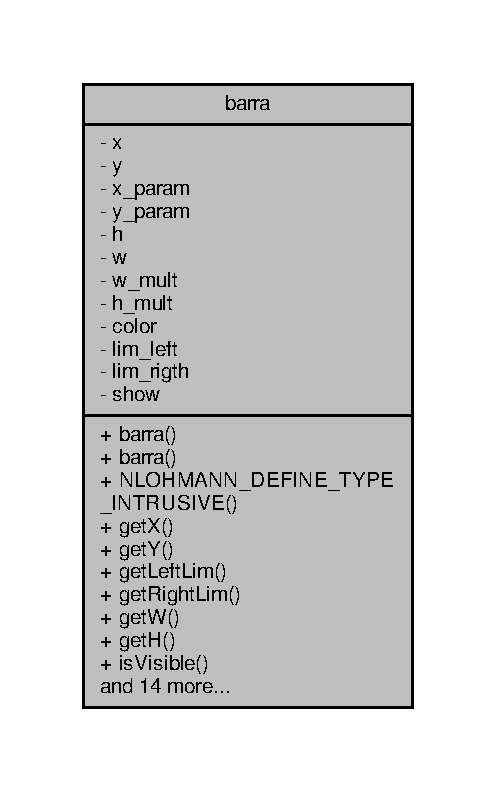
\includegraphics[width=154pt]{classbarra__coll__graph}
\end{center}
\end{figure}
\subsection*{Public Member Functions}
\begin{DoxyCompactItemize}
\item 
\hyperlink{classbarra_a5acfb9b82a30794e040d4f156562317c}{barra} (int x\+\_\+, int y\+\_\+)
\begin{DoxyCompactList}\small\item\em Construtor da barra. \end{DoxyCompactList}\item 
int \hyperlink{classbarra_a2f3787aab4304ccd3e5ac813d5387f26}{getX} ()
\item 
int \hyperlink{classbarra_a5eed7412b3afaa38f74ab8ce2e3cf80c}{getY} ()
\item 
int \hyperlink{classbarra_aad00b16b2f10c8f2e9b11981c44037c6}{getW} ()
\item 
int \hyperlink{classbarra_a640467fe10e4d76eba2cdddf560ac08a}{getH} ()
\item 
float \hyperlink{classbarra_a2e8656df299ddc913bcacac2505a6733}{get\+Wmult} ()
\item 
float \hyperlink{classbarra_ac3e797dcb0cfdeba9cb3ff813f16021e}{get\+Hmult} ()
\item 
void \hyperlink{classbarra_a1653a2f02c5c429afac46845ab35b50f}{setW} (int w\+\_\+)
\item 
void \hyperlink{classbarra_a527670e645cee76fd476f0fd731040a4}{setH} (int h\+\_\+)
\item 
void \hyperlink{classbarra_a9b3d595be05ea5ddb56f3f0b598dbb0b}{setX} (int x\+\_\+)
\item 
void \hyperlink{classbarra_a3571249441c47aa48766ab10fec170ad}{setY} (int y\+\_\+)
\end{DoxyCompactItemize}
\subsection*{Private Attributes}
\begin{DoxyCompactItemize}
\item 
int \hyperlink{classbarra_a60f0c711fd29434f3fb07a3f584a83a1}{x}
\item 
int \hyperlink{classbarra_a93b604008af3593ac1b80366c387f2e9}{y}
\item 
int \hyperlink{classbarra_add2a64a98c1781d1cc9b7b1f744df1a5}{h}
\item 
int \hyperlink{classbarra_a31fd53ae11742f912eb9e0b20707cb82}{w}
\item 
float \hyperlink{classbarra_a7ca620e27ef6e75eb8dfcc05a738a97c}{w\+\_\+mult} = 2
\item 
float \hyperlink{classbarra_a6ee439263b66198984d59f0ef128e7a6}{h\+\_\+mult} = 0.\+25
\item 
int \hyperlink{classbarra_a7234eb8aa0b635f9c1fb0456ebd7901c}{color}
\end{DoxyCompactItemize}


\subsection{Detailed Description}
Classe para a barra. 

Esta é a classe para a barra. Ela possui variaveis internas para guardar suas dimensoes e posicao, alem de ter um fator de multiplicacao para quando for ser mostrada na tela. 

\subsection{Constructor \& Destructor Documentation}
\index{barra@{barra}!barra@{barra}}
\index{barra@{barra}!barra@{barra}}
\subsubsection[{\texorpdfstring{barra(int x\+\_\+, int y\+\_\+)}{barra(int x_, int y_)}}]{\setlength{\rightskip}{0pt plus 5cm}barra\+::barra (
\begin{DoxyParamCaption}
\item[{int}]{x\+\_\+, }
\item[{int}]{y\+\_\+}
\end{DoxyParamCaption}
)}\hypertarget{classbarra_a5acfb9b82a30794e040d4f156562317c}{}\label{classbarra_a5acfb9b82a30794e040d4f156562317c}


Construtor da barra. 

Recebe uma posicao (x,y) inicial da barra 

\subsection{Member Function Documentation}
\index{barra@{barra}!getH@{getH}}
\index{getH@{getH}!barra@{barra}}
\subsubsection[{\texorpdfstring{get\+H()}{getH()}}]{\setlength{\rightskip}{0pt plus 5cm}int barra\+::getH (
\begin{DoxyParamCaption}
{}
\end{DoxyParamCaption}
)}\hypertarget{classbarra_a640467fe10e4d76eba2cdddf560ac08a}{}\label{classbarra_a640467fe10e4d76eba2cdddf560ac08a}
\index{barra@{barra}!get\+Hmult@{get\+Hmult}}
\index{get\+Hmult@{get\+Hmult}!barra@{barra}}
\subsubsection[{\texorpdfstring{get\+Hmult()}{getHmult()}}]{\setlength{\rightskip}{0pt plus 5cm}float barra\+::get\+Hmult (
\begin{DoxyParamCaption}
{}
\end{DoxyParamCaption}
)}\hypertarget{classbarra_ac3e797dcb0cfdeba9cb3ff813f16021e}{}\label{classbarra_ac3e797dcb0cfdeba9cb3ff813f16021e}
\index{barra@{barra}!getW@{getW}}
\index{getW@{getW}!barra@{barra}}
\subsubsection[{\texorpdfstring{get\+W()}{getW()}}]{\setlength{\rightskip}{0pt plus 5cm}int barra\+::getW (
\begin{DoxyParamCaption}
{}
\end{DoxyParamCaption}
)}\hypertarget{classbarra_aad00b16b2f10c8f2e9b11981c44037c6}{}\label{classbarra_aad00b16b2f10c8f2e9b11981c44037c6}
\index{barra@{barra}!get\+Wmult@{get\+Wmult}}
\index{get\+Wmult@{get\+Wmult}!barra@{barra}}
\subsubsection[{\texorpdfstring{get\+Wmult()}{getWmult()}}]{\setlength{\rightskip}{0pt plus 5cm}float barra\+::get\+Wmult (
\begin{DoxyParamCaption}
{}
\end{DoxyParamCaption}
)}\hypertarget{classbarra_a2e8656df299ddc913bcacac2505a6733}{}\label{classbarra_a2e8656df299ddc913bcacac2505a6733}
\index{barra@{barra}!getX@{getX}}
\index{getX@{getX}!barra@{barra}}
\subsubsection[{\texorpdfstring{get\+X()}{getX()}}]{\setlength{\rightskip}{0pt plus 5cm}int barra\+::getX (
\begin{DoxyParamCaption}
{}
\end{DoxyParamCaption}
)}\hypertarget{classbarra_a2f3787aab4304ccd3e5ac813d5387f26}{}\label{classbarra_a2f3787aab4304ccd3e5ac813d5387f26}
\index{barra@{barra}!getY@{getY}}
\index{getY@{getY}!barra@{barra}}
\subsubsection[{\texorpdfstring{get\+Y()}{getY()}}]{\setlength{\rightskip}{0pt plus 5cm}int barra\+::getY (
\begin{DoxyParamCaption}
{}
\end{DoxyParamCaption}
)}\hypertarget{classbarra_a5eed7412b3afaa38f74ab8ce2e3cf80c}{}\label{classbarra_a5eed7412b3afaa38f74ab8ce2e3cf80c}
\index{barra@{barra}!setH@{setH}}
\index{setH@{setH}!barra@{barra}}
\subsubsection[{\texorpdfstring{set\+H(int h\+\_\+)}{setH(int h_)}}]{\setlength{\rightskip}{0pt plus 5cm}void barra\+::setH (
\begin{DoxyParamCaption}
\item[{int}]{h\+\_\+}
\end{DoxyParamCaption}
)}\hypertarget{classbarra_a527670e645cee76fd476f0fd731040a4}{}\label{classbarra_a527670e645cee76fd476f0fd731040a4}
\index{barra@{barra}!setW@{setW}}
\index{setW@{setW}!barra@{barra}}
\subsubsection[{\texorpdfstring{set\+W(int w\+\_\+)}{setW(int w_)}}]{\setlength{\rightskip}{0pt plus 5cm}void barra\+::setW (
\begin{DoxyParamCaption}
\item[{int}]{w\+\_\+}
\end{DoxyParamCaption}
)}\hypertarget{classbarra_a1653a2f02c5c429afac46845ab35b50f}{}\label{classbarra_a1653a2f02c5c429afac46845ab35b50f}
\index{barra@{barra}!setX@{setX}}
\index{setX@{setX}!barra@{barra}}
\subsubsection[{\texorpdfstring{set\+X(int x\+\_\+)}{setX(int x_)}}]{\setlength{\rightskip}{0pt plus 5cm}void barra\+::setX (
\begin{DoxyParamCaption}
\item[{int}]{x\+\_\+}
\end{DoxyParamCaption}
)}\hypertarget{classbarra_a9b3d595be05ea5ddb56f3f0b598dbb0b}{}\label{classbarra_a9b3d595be05ea5ddb56f3f0b598dbb0b}
\index{barra@{barra}!setY@{setY}}
\index{setY@{setY}!barra@{barra}}
\subsubsection[{\texorpdfstring{set\+Y(int y\+\_\+)}{setY(int y_)}}]{\setlength{\rightskip}{0pt plus 5cm}void barra\+::setY (
\begin{DoxyParamCaption}
\item[{int}]{y\+\_\+}
\end{DoxyParamCaption}
)}\hypertarget{classbarra_a3571249441c47aa48766ab10fec170ad}{}\label{classbarra_a3571249441c47aa48766ab10fec170ad}


\subsection{Member Data Documentation}
\index{barra@{barra}!color@{color}}
\index{color@{color}!barra@{barra}}
\subsubsection[{\texorpdfstring{color}{color}}]{\setlength{\rightskip}{0pt plus 5cm}int barra\+::color\hspace{0.3cm}{\ttfamily [private]}}\hypertarget{classbarra_a7234eb8aa0b635f9c1fb0456ebd7901c}{}\label{classbarra_a7234eb8aa0b635f9c1fb0456ebd7901c}
Cor da barra \index{barra@{barra}!h@{h}}
\index{h@{h}!barra@{barra}}
\subsubsection[{\texorpdfstring{h}{h}}]{\setlength{\rightskip}{0pt plus 5cm}int barra\+::h\hspace{0.3cm}{\ttfamily [private]}}\hypertarget{classbarra_add2a64a98c1781d1cc9b7b1f744df1a5}{}\label{classbarra_add2a64a98c1781d1cc9b7b1f744df1a5}
\index{barra@{barra}!h\+\_\+mult@{h\+\_\+mult}}
\index{h\+\_\+mult@{h\+\_\+mult}!barra@{barra}}
\subsubsection[{\texorpdfstring{h\+\_\+mult}{h_mult}}]{\setlength{\rightskip}{0pt plus 5cm}float barra\+::h\+\_\+mult = 0.\+25\hspace{0.3cm}{\ttfamily [private]}}\hypertarget{classbarra_a6ee439263b66198984d59f0ef128e7a6}{}\label{classbarra_a6ee439263b66198984d59f0ef128e7a6}
Fator de multiplicacao para visualizacao \index{barra@{barra}!w@{w}}
\index{w@{w}!barra@{barra}}
\subsubsection[{\texorpdfstring{w}{w}}]{\setlength{\rightskip}{0pt plus 5cm}int barra\+::w\hspace{0.3cm}{\ttfamily [private]}}\hypertarget{classbarra_a31fd53ae11742f912eb9e0b20707cb82}{}\label{classbarra_a31fd53ae11742f912eb9e0b20707cb82}
Variaveis de dimensao \index{barra@{barra}!w\+\_\+mult@{w\+\_\+mult}}
\index{w\+\_\+mult@{w\+\_\+mult}!barra@{barra}}
\subsubsection[{\texorpdfstring{w\+\_\+mult}{w_mult}}]{\setlength{\rightskip}{0pt plus 5cm}float barra\+::w\+\_\+mult = 2\hspace{0.3cm}{\ttfamily [private]}}\hypertarget{classbarra_a7ca620e27ef6e75eb8dfcc05a738a97c}{}\label{classbarra_a7ca620e27ef6e75eb8dfcc05a738a97c}
\index{barra@{barra}!x@{x}}
\index{x@{x}!barra@{barra}}
\subsubsection[{\texorpdfstring{x}{x}}]{\setlength{\rightskip}{0pt plus 5cm}int barra\+::x\hspace{0.3cm}{\ttfamily [private]}}\hypertarget{classbarra_a60f0c711fd29434f3fb07a3f584a83a1}{}\label{classbarra_a60f0c711fd29434f3fb07a3f584a83a1}
\index{barra@{barra}!y@{y}}
\index{y@{y}!barra@{barra}}
\subsubsection[{\texorpdfstring{y}{y}}]{\setlength{\rightskip}{0pt plus 5cm}int barra\+::y\hspace{0.3cm}{\ttfamily [private]}}\hypertarget{classbarra_a93b604008af3593ac1b80366c387f2e9}{}\label{classbarra_a93b604008af3593ac1b80366c387f2e9}
Variaveis de posicao 

The documentation for this class was generated from the following files\+:\begin{DoxyCompactItemize}
\item 
include/\hyperlink{barra_8h}{barra.\+h}\item 
src/model/\hyperlink{barra_8cpp}{barra.\+cpp}\end{DoxyCompactItemize}

\hypertarget{classbolinha}{}\section{bolinha Class Reference}
\label{classbolinha}\index{bolinha@{bolinha}}


Classe para a bolinha.  




{\ttfamily \#include $<$bolinha.\+h$>$}



Collaboration diagram for bolinha\+:
\nopagebreak
\begin{figure}[H]
\begin{center}
\leavevmode
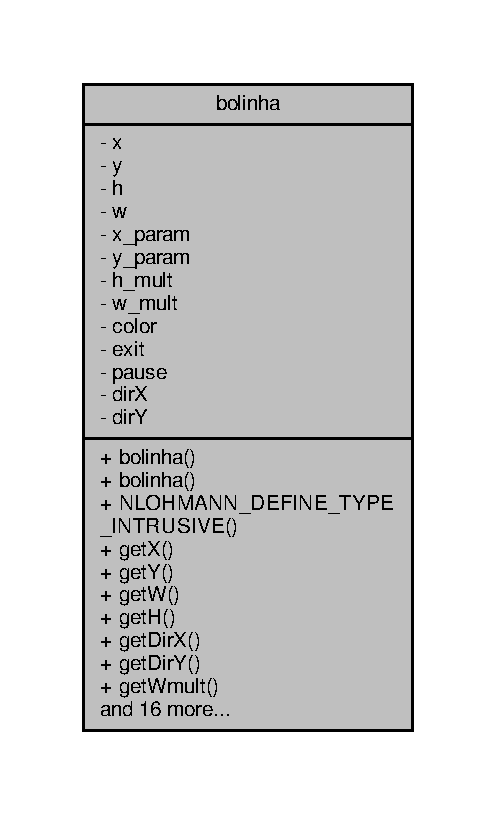
\includegraphics[width=238pt]{classbolinha__coll__graph}
\end{center}
\end{figure}
\subsection*{Public Member Functions}
\begin{DoxyCompactItemize}
\item 
\hyperlink{classbolinha_a157417fa65cf082083216e56ddab736a}{bolinha} (int x\+\_\+, int y\+\_\+)
\begin{DoxyCompactList}\small\item\em Construtor da bolinha. \end{DoxyCompactList}\item 
\hyperlink{classbolinha_afd9c0cf1e0c6fc54ebac1c950fdb182d}{bolinha} ()
\item 
\hyperlink{classbolinha_ad14e4c36911a540dd4e0b23125c2c489}{N\+L\+O\+H\+M\+A\+N\+N\+\_\+\+D\+E\+F\+I\+N\+E\+\_\+\+T\+Y\+P\+E\+\_\+\+I\+N\+T\+R\+U\+S\+I\+VE} (\hyperlink{classbolinha}{bolinha}, \hyperlink{classbolinha_ad6918f0b95a774318e4ceb7c3f9720de}{x}, \hyperlink{classbolinha_a1ef5bc9948639dc0065e17a8e6b88846}{y}, \hyperlink{classbolinha_a0e4ccf4bf9cd1b980323dbcba247ca8b}{dirX}, \hyperlink{classbolinha_a9ed43eedc9ce54d9645824b4a876171e}{dirY}, \hyperlink{classbolinha_a4136d7cb978a3190073e1544fb336876}{w}, \hyperlink{classbolinha_a971dc9047d1dcc5fd7cf4c4ed945de45}{h}, \hyperlink{classbolinha_ac9d2238772d85a88f57602ff7bfd8387}{x\+\_\+param}, \hyperlink{classbolinha_a2fe551614672e64a4f34ecdd226de4ca}{y\+\_\+param})
\item 
int \hyperlink{classbolinha_a16bfb1ab48a09a3dd5cf5868cb2f475d}{getX} ()
\item 
int \hyperlink{classbolinha_a143dbe11a42e1fcdccb1f19d4d9f715e}{getY} ()
\item 
int \hyperlink{classbolinha_ab5cbca5168da5df74705fea330490382}{getW} ()
\item 
int \hyperlink{classbolinha_ae6c9c0d7b5770ca865e1bd5cc1f773f4}{getH} ()
\item 
int \hyperlink{classbolinha_acb37ecbc6681ac8cc433e21a8fe77328}{get\+DirX} ()
\item 
int \hyperlink{classbolinha_af41c7d6e46fcdd428de4e726dbcf5f3a}{get\+DirY} ()
\item 
float \hyperlink{classbolinha_a90342ef3d458c503db81dd80c53ffa05}{get\+Wmult} ()
\item 
float \hyperlink{classbolinha_ac485ff1907f1416a42511d0d333eef59}{get\+Hmult} ()
\item 
bool \hyperlink{classbolinha_a87e092bdaa996f8c08236d3e3aa4c605}{get\+Exit} ()
\item 
bool \hyperlink{classbolinha_a416b5ee9e822606a0cc414f384619000}{get\+Pause} ()
\item 
float \hyperlink{classbolinha_af48d96c4fa8552bd44e9c5f3bb1724a5}{get\+Xparam} ()
\item 
float \hyperlink{classbolinha_a15fa13bcfd66f43b2e7c5f1d8416ea15}{get\+Yparam} ()
\item 
void \hyperlink{classbolinha_a92da76fdb57264e2edc33d96ddb3e4d4}{set\+Xparam} (float x\+\_\+param\+\_\+)
\item 
void \hyperlink{classbolinha_accc5d5fe698a340c6b085e3dad3d1af9}{set\+Yparam} (float y\+\_\+param\+\_\+)
\item 
void \hyperlink{classbolinha_aa96439a9d3655912359a58a2096f8adc}{setX} (int x\+\_\+)
\item 
void \hyperlink{classbolinha_a28c1acdaebe902ba404ac6873800d8bf}{setY} (int y\+\_\+)
\item 
void \hyperlink{classbolinha_a2196da39c838309cf723b1c25789deb0}{set\+DirX} (int dir\+X\+\_\+)
\item 
void \hyperlink{classbolinha_a6beb9dba4c6de15d103a9827cf5ea7c7}{set\+DirY} (int dir\+Y\+\_\+)
\item 
void \hyperlink{classbolinha_a67d6d1e736779f2bbc845860103cc8fc}{setW} (int w\+\_\+)
\item 
void \hyperlink{classbolinha_ac77f2965fe5b0fab4879d5eeb89b1560}{setH} (int h\+\_\+)
\item 
void \hyperlink{classbolinha_a69c7848b06c9436027e3e1d117b03b26}{set\+Exit} (bool exit\+\_\+)
\item 
void \hyperlink{classbolinha_af223163ae42634912c3e4cba05e48acd}{set\+Pause} (bool pause\+\_\+)
\item 
std\+::string \hyperlink{classbolinha_a046ccfd6e883d8f6d2c9501459ab89d1}{print} ()
\end{DoxyCompactItemize}
\subsection*{Private Attributes}
\begin{DoxyCompactItemize}
\item 
int \hyperlink{classbolinha_ad6918f0b95a774318e4ceb7c3f9720de}{x}
\item 
int \hyperlink{classbolinha_a1ef5bc9948639dc0065e17a8e6b88846}{y}
\item 
int \hyperlink{classbolinha_a971dc9047d1dcc5fd7cf4c4ed945de45}{h}
\item 
int \hyperlink{classbolinha_a4136d7cb978a3190073e1544fb336876}{w}
\item 
float \hyperlink{classbolinha_ac9d2238772d85a88f57602ff7bfd8387}{x\+\_\+param}
\item 
float \hyperlink{classbolinha_a2fe551614672e64a4f34ecdd226de4ca}{y\+\_\+param}
\item 
float \hyperlink{classbolinha_add6888f6be8396c001dfa10e15d6a4be}{h\+\_\+mult} =0.\+25
\item 
float \hyperlink{classbolinha_a91dd1f60f5312cf476e02e5396c2f871}{w\+\_\+mult} =0.\+25
\item 
int \hyperlink{classbolinha_af44eba52e992cb2ed5787bce3256dca1}{color}
\item 
bool \hyperlink{classbolinha_a29132ebeca6235fa17c303151622cd3b}{exit} = false
\item 
bool \hyperlink{classbolinha_a85326b85a811e46b6d98c900e141b0ef}{pause} = false
\item 
int \hyperlink{classbolinha_a0e4ccf4bf9cd1b980323dbcba247ca8b}{dirX} = 5
\item 
int \hyperlink{classbolinha_a9ed43eedc9ce54d9645824b4a876171e}{dirY} = 5
\end{DoxyCompactItemize}


\subsection{Detailed Description}
Classe para a bolinha. 

Esta é a classe para a bolinha. Ela possui variaveis internas para guardar suas dimensoes e posicao, alem de ter um fator de multiplicacao para quando for ser mostrada na tela. Tambem tem os parametros de estado exit e pause 

\subsection{Constructor \& Destructor Documentation}
\index{bolinha@{bolinha}!bolinha@{bolinha}}
\index{bolinha@{bolinha}!bolinha@{bolinha}}
\subsubsection[{\texorpdfstring{bolinha(int x\+\_\+, int y\+\_\+)}{bolinha(int x_, int y_)}}]{\setlength{\rightskip}{0pt plus 5cm}bolinha\+::bolinha (
\begin{DoxyParamCaption}
\item[{int}]{x\+\_\+, }
\item[{int}]{y\+\_\+}
\end{DoxyParamCaption}
)}\hypertarget{classbolinha_a157417fa65cf082083216e56ddab736a}{}\label{classbolinha_a157417fa65cf082083216e56ddab736a}


Construtor da bolinha. 

Recebe uma posicao (x,y) inicial da bolinha \index{bolinha@{bolinha}!bolinha@{bolinha}}
\index{bolinha@{bolinha}!bolinha@{bolinha}}
\subsubsection[{\texorpdfstring{bolinha()}{bolinha()}}]{\setlength{\rightskip}{0pt plus 5cm}bolinha\+::bolinha (
\begin{DoxyParamCaption}
{}
\end{DoxyParamCaption}
)}\hypertarget{classbolinha_afd9c0cf1e0c6fc54ebac1c950fdb182d}{}\label{classbolinha_afd9c0cf1e0c6fc54ebac1c950fdb182d}


\subsection{Member Function Documentation}
\index{bolinha@{bolinha}!get\+DirX@{get\+DirX}}
\index{get\+DirX@{get\+DirX}!bolinha@{bolinha}}
\subsubsection[{\texorpdfstring{get\+Dir\+X()}{getDirX()}}]{\setlength{\rightskip}{0pt plus 5cm}int bolinha\+::get\+DirX (
\begin{DoxyParamCaption}
{}
\end{DoxyParamCaption}
)}\hypertarget{classbolinha_acb37ecbc6681ac8cc433e21a8fe77328}{}\label{classbolinha_acb37ecbc6681ac8cc433e21a8fe77328}
\index{bolinha@{bolinha}!get\+DirY@{get\+DirY}}
\index{get\+DirY@{get\+DirY}!bolinha@{bolinha}}
\subsubsection[{\texorpdfstring{get\+Dir\+Y()}{getDirY()}}]{\setlength{\rightskip}{0pt plus 5cm}int bolinha\+::get\+DirY (
\begin{DoxyParamCaption}
{}
\end{DoxyParamCaption}
)}\hypertarget{classbolinha_af41c7d6e46fcdd428de4e726dbcf5f3a}{}\label{classbolinha_af41c7d6e46fcdd428de4e726dbcf5f3a}
\index{bolinha@{bolinha}!get\+Exit@{get\+Exit}}
\index{get\+Exit@{get\+Exit}!bolinha@{bolinha}}
\subsubsection[{\texorpdfstring{get\+Exit()}{getExit()}}]{\setlength{\rightskip}{0pt plus 5cm}bool bolinha\+::get\+Exit (
\begin{DoxyParamCaption}
{}
\end{DoxyParamCaption}
)}\hypertarget{classbolinha_a87e092bdaa996f8c08236d3e3aa4c605}{}\label{classbolinha_a87e092bdaa996f8c08236d3e3aa4c605}
\index{bolinha@{bolinha}!getH@{getH}}
\index{getH@{getH}!bolinha@{bolinha}}
\subsubsection[{\texorpdfstring{get\+H()}{getH()}}]{\setlength{\rightskip}{0pt plus 5cm}int bolinha\+::getH (
\begin{DoxyParamCaption}
{}
\end{DoxyParamCaption}
)}\hypertarget{classbolinha_ae6c9c0d7b5770ca865e1bd5cc1f773f4}{}\label{classbolinha_ae6c9c0d7b5770ca865e1bd5cc1f773f4}
\index{bolinha@{bolinha}!get\+Hmult@{get\+Hmult}}
\index{get\+Hmult@{get\+Hmult}!bolinha@{bolinha}}
\subsubsection[{\texorpdfstring{get\+Hmult()}{getHmult()}}]{\setlength{\rightskip}{0pt plus 5cm}float bolinha\+::get\+Hmult (
\begin{DoxyParamCaption}
{}
\end{DoxyParamCaption}
)}\hypertarget{classbolinha_ac485ff1907f1416a42511d0d333eef59}{}\label{classbolinha_ac485ff1907f1416a42511d0d333eef59}
\index{bolinha@{bolinha}!get\+Pause@{get\+Pause}}
\index{get\+Pause@{get\+Pause}!bolinha@{bolinha}}
\subsubsection[{\texorpdfstring{get\+Pause()}{getPause()}}]{\setlength{\rightskip}{0pt plus 5cm}bool bolinha\+::get\+Pause (
\begin{DoxyParamCaption}
{}
\end{DoxyParamCaption}
)}\hypertarget{classbolinha_a416b5ee9e822606a0cc414f384619000}{}\label{classbolinha_a416b5ee9e822606a0cc414f384619000}
\index{bolinha@{bolinha}!getW@{getW}}
\index{getW@{getW}!bolinha@{bolinha}}
\subsubsection[{\texorpdfstring{get\+W()}{getW()}}]{\setlength{\rightskip}{0pt plus 5cm}int bolinha\+::getW (
\begin{DoxyParamCaption}
{}
\end{DoxyParamCaption}
)}\hypertarget{classbolinha_ab5cbca5168da5df74705fea330490382}{}\label{classbolinha_ab5cbca5168da5df74705fea330490382}
\index{bolinha@{bolinha}!get\+Wmult@{get\+Wmult}}
\index{get\+Wmult@{get\+Wmult}!bolinha@{bolinha}}
\subsubsection[{\texorpdfstring{get\+Wmult()}{getWmult()}}]{\setlength{\rightskip}{0pt plus 5cm}float bolinha\+::get\+Wmult (
\begin{DoxyParamCaption}
{}
\end{DoxyParamCaption}
)}\hypertarget{classbolinha_a90342ef3d458c503db81dd80c53ffa05}{}\label{classbolinha_a90342ef3d458c503db81dd80c53ffa05}
\index{bolinha@{bolinha}!getX@{getX}}
\index{getX@{getX}!bolinha@{bolinha}}
\subsubsection[{\texorpdfstring{get\+X()}{getX()}}]{\setlength{\rightskip}{0pt plus 5cm}int bolinha\+::getX (
\begin{DoxyParamCaption}
{}
\end{DoxyParamCaption}
)}\hypertarget{classbolinha_a16bfb1ab48a09a3dd5cf5868cb2f475d}{}\label{classbolinha_a16bfb1ab48a09a3dd5cf5868cb2f475d}
\index{bolinha@{bolinha}!get\+Xparam@{get\+Xparam}}
\index{get\+Xparam@{get\+Xparam}!bolinha@{bolinha}}
\subsubsection[{\texorpdfstring{get\+Xparam()}{getXparam()}}]{\setlength{\rightskip}{0pt plus 5cm}float bolinha\+::get\+Xparam (
\begin{DoxyParamCaption}
{}
\end{DoxyParamCaption}
)}\hypertarget{classbolinha_af48d96c4fa8552bd44e9c5f3bb1724a5}{}\label{classbolinha_af48d96c4fa8552bd44e9c5f3bb1724a5}
\index{bolinha@{bolinha}!getY@{getY}}
\index{getY@{getY}!bolinha@{bolinha}}
\subsubsection[{\texorpdfstring{get\+Y()}{getY()}}]{\setlength{\rightskip}{0pt plus 5cm}int bolinha\+::getY (
\begin{DoxyParamCaption}
{}
\end{DoxyParamCaption}
)}\hypertarget{classbolinha_a143dbe11a42e1fcdccb1f19d4d9f715e}{}\label{classbolinha_a143dbe11a42e1fcdccb1f19d4d9f715e}
\index{bolinha@{bolinha}!get\+Yparam@{get\+Yparam}}
\index{get\+Yparam@{get\+Yparam}!bolinha@{bolinha}}
\subsubsection[{\texorpdfstring{get\+Yparam()}{getYparam()}}]{\setlength{\rightskip}{0pt plus 5cm}float bolinha\+::get\+Yparam (
\begin{DoxyParamCaption}
{}
\end{DoxyParamCaption}
)}\hypertarget{classbolinha_a15fa13bcfd66f43b2e7c5f1d8416ea15}{}\label{classbolinha_a15fa13bcfd66f43b2e7c5f1d8416ea15}
\index{bolinha@{bolinha}!N\+L\+O\+H\+M\+A\+N\+N\+\_\+\+D\+E\+F\+I\+N\+E\+\_\+\+T\+Y\+P\+E\+\_\+\+I\+N\+T\+R\+U\+S\+I\+VE@{N\+L\+O\+H\+M\+A\+N\+N\+\_\+\+D\+E\+F\+I\+N\+E\+\_\+\+T\+Y\+P\+E\+\_\+\+I\+N\+T\+R\+U\+S\+I\+VE}}
\index{N\+L\+O\+H\+M\+A\+N\+N\+\_\+\+D\+E\+F\+I\+N\+E\+\_\+\+T\+Y\+P\+E\+\_\+\+I\+N\+T\+R\+U\+S\+I\+VE@{N\+L\+O\+H\+M\+A\+N\+N\+\_\+\+D\+E\+F\+I\+N\+E\+\_\+\+T\+Y\+P\+E\+\_\+\+I\+N\+T\+R\+U\+S\+I\+VE}!bolinha@{bolinha}}
\subsubsection[{\texorpdfstring{N\+L\+O\+H\+M\+A\+N\+N\+\_\+\+D\+E\+F\+I\+N\+E\+\_\+\+T\+Y\+P\+E\+\_\+\+I\+N\+T\+R\+U\+S\+I\+V\+E(bolinha, x, y, dir\+X, dir\+Y, w, h, x\+\_\+param, y\+\_\+param)}{NLOHMANN_DEFINE_TYPE_INTRUSIVE(bolinha, x, y, dirX, dirY, w, h, x_param, y_param)}}]{\setlength{\rightskip}{0pt plus 5cm}bolinha\+::\+N\+L\+O\+H\+M\+A\+N\+N\+\_\+\+D\+E\+F\+I\+N\+E\+\_\+\+T\+Y\+P\+E\+\_\+\+I\+N\+T\+R\+U\+S\+I\+VE (
\begin{DoxyParamCaption}
\item[{{\bf bolinha}}]{, }
\item[{{\bf x}}]{, }
\item[{{\bf y}}]{, }
\item[{{\bf dirX}}]{, }
\item[{{\bf dirY}}]{, }
\item[{{\bf w}}]{, }
\item[{{\bf h}}]{, }
\item[{{\bf x\+\_\+param}}]{, }
\item[{{\bf y\+\_\+param}}]{}
\end{DoxyParamCaption}
)}\hypertarget{classbolinha_ad14e4c36911a540dd4e0b23125c2c489}{}\label{classbolinha_ad14e4c36911a540dd4e0b23125c2c489}
\index{bolinha@{bolinha}!print@{print}}
\index{print@{print}!bolinha@{bolinha}}
\subsubsection[{\texorpdfstring{print()}{print()}}]{\setlength{\rightskip}{0pt plus 5cm}std\+::string bolinha\+::print (
\begin{DoxyParamCaption}
{}
\end{DoxyParamCaption}
)}\hypertarget{classbolinha_a046ccfd6e883d8f6d2c9501459ab89d1}{}\label{classbolinha_a046ccfd6e883d8f6d2c9501459ab89d1}
\index{bolinha@{bolinha}!set\+DirX@{set\+DirX}}
\index{set\+DirX@{set\+DirX}!bolinha@{bolinha}}
\subsubsection[{\texorpdfstring{set\+Dir\+X(int dir\+X\+\_\+)}{setDirX(int dirX_)}}]{\setlength{\rightskip}{0pt plus 5cm}void bolinha\+::set\+DirX (
\begin{DoxyParamCaption}
\item[{int}]{dir\+X\+\_\+}
\end{DoxyParamCaption}
)}\hypertarget{classbolinha_a2196da39c838309cf723b1c25789deb0}{}\label{classbolinha_a2196da39c838309cf723b1c25789deb0}
\index{bolinha@{bolinha}!set\+DirY@{set\+DirY}}
\index{set\+DirY@{set\+DirY}!bolinha@{bolinha}}
\subsubsection[{\texorpdfstring{set\+Dir\+Y(int dir\+Y\+\_\+)}{setDirY(int dirY_)}}]{\setlength{\rightskip}{0pt plus 5cm}void bolinha\+::set\+DirY (
\begin{DoxyParamCaption}
\item[{int}]{dir\+Y\+\_\+}
\end{DoxyParamCaption}
)}\hypertarget{classbolinha_a6beb9dba4c6de15d103a9827cf5ea7c7}{}\label{classbolinha_a6beb9dba4c6de15d103a9827cf5ea7c7}
\index{bolinha@{bolinha}!set\+Exit@{set\+Exit}}
\index{set\+Exit@{set\+Exit}!bolinha@{bolinha}}
\subsubsection[{\texorpdfstring{set\+Exit(bool exit\+\_\+)}{setExit(bool exit_)}}]{\setlength{\rightskip}{0pt plus 5cm}void bolinha\+::set\+Exit (
\begin{DoxyParamCaption}
\item[{bool}]{exit\+\_\+}
\end{DoxyParamCaption}
)}\hypertarget{classbolinha_a69c7848b06c9436027e3e1d117b03b26}{}\label{classbolinha_a69c7848b06c9436027e3e1d117b03b26}
\index{bolinha@{bolinha}!setH@{setH}}
\index{setH@{setH}!bolinha@{bolinha}}
\subsubsection[{\texorpdfstring{set\+H(int h\+\_\+)}{setH(int h_)}}]{\setlength{\rightskip}{0pt plus 5cm}void bolinha\+::setH (
\begin{DoxyParamCaption}
\item[{int}]{h\+\_\+}
\end{DoxyParamCaption}
)}\hypertarget{classbolinha_ac77f2965fe5b0fab4879d5eeb89b1560}{}\label{classbolinha_ac77f2965fe5b0fab4879d5eeb89b1560}
\index{bolinha@{bolinha}!set\+Pause@{set\+Pause}}
\index{set\+Pause@{set\+Pause}!bolinha@{bolinha}}
\subsubsection[{\texorpdfstring{set\+Pause(bool pause\+\_\+)}{setPause(bool pause_)}}]{\setlength{\rightskip}{0pt plus 5cm}void bolinha\+::set\+Pause (
\begin{DoxyParamCaption}
\item[{bool}]{pause\+\_\+}
\end{DoxyParamCaption}
)}\hypertarget{classbolinha_af223163ae42634912c3e4cba05e48acd}{}\label{classbolinha_af223163ae42634912c3e4cba05e48acd}
\index{bolinha@{bolinha}!setW@{setW}}
\index{setW@{setW}!bolinha@{bolinha}}
\subsubsection[{\texorpdfstring{set\+W(int w\+\_\+)}{setW(int w_)}}]{\setlength{\rightskip}{0pt plus 5cm}void bolinha\+::setW (
\begin{DoxyParamCaption}
\item[{int}]{w\+\_\+}
\end{DoxyParamCaption}
)}\hypertarget{classbolinha_a67d6d1e736779f2bbc845860103cc8fc}{}\label{classbolinha_a67d6d1e736779f2bbc845860103cc8fc}
\index{bolinha@{bolinha}!setX@{setX}}
\index{setX@{setX}!bolinha@{bolinha}}
\subsubsection[{\texorpdfstring{set\+X(int x\+\_\+)}{setX(int x_)}}]{\setlength{\rightskip}{0pt plus 5cm}void bolinha\+::setX (
\begin{DoxyParamCaption}
\item[{int}]{x\+\_\+}
\end{DoxyParamCaption}
)}\hypertarget{classbolinha_aa96439a9d3655912359a58a2096f8adc}{}\label{classbolinha_aa96439a9d3655912359a58a2096f8adc}
\index{bolinha@{bolinha}!set\+Xparam@{set\+Xparam}}
\index{set\+Xparam@{set\+Xparam}!bolinha@{bolinha}}
\subsubsection[{\texorpdfstring{set\+Xparam(float x\+\_\+param\+\_\+)}{setXparam(float x_param_)}}]{\setlength{\rightskip}{0pt plus 5cm}void bolinha\+::set\+Xparam (
\begin{DoxyParamCaption}
\item[{float}]{x\+\_\+param\+\_\+}
\end{DoxyParamCaption}
)}\hypertarget{classbolinha_a92da76fdb57264e2edc33d96ddb3e4d4}{}\label{classbolinha_a92da76fdb57264e2edc33d96ddb3e4d4}
\index{bolinha@{bolinha}!setY@{setY}}
\index{setY@{setY}!bolinha@{bolinha}}
\subsubsection[{\texorpdfstring{set\+Y(int y\+\_\+)}{setY(int y_)}}]{\setlength{\rightskip}{0pt plus 5cm}void bolinha\+::setY (
\begin{DoxyParamCaption}
\item[{int}]{y\+\_\+}
\end{DoxyParamCaption}
)}\hypertarget{classbolinha_a28c1acdaebe902ba404ac6873800d8bf}{}\label{classbolinha_a28c1acdaebe902ba404ac6873800d8bf}
\index{bolinha@{bolinha}!set\+Yparam@{set\+Yparam}}
\index{set\+Yparam@{set\+Yparam}!bolinha@{bolinha}}
\subsubsection[{\texorpdfstring{set\+Yparam(float y\+\_\+param\+\_\+)}{setYparam(float y_param_)}}]{\setlength{\rightskip}{0pt plus 5cm}void bolinha\+::set\+Yparam (
\begin{DoxyParamCaption}
\item[{float}]{y\+\_\+param\+\_\+}
\end{DoxyParamCaption}
)}\hypertarget{classbolinha_accc5d5fe698a340c6b085e3dad3d1af9}{}\label{classbolinha_accc5d5fe698a340c6b085e3dad3d1af9}


\subsection{Member Data Documentation}
\index{bolinha@{bolinha}!color@{color}}
\index{color@{color}!bolinha@{bolinha}}
\subsubsection[{\texorpdfstring{color}{color}}]{\setlength{\rightskip}{0pt plus 5cm}int bolinha\+::color\hspace{0.3cm}{\ttfamily [private]}}\hypertarget{classbolinha_af44eba52e992cb2ed5787bce3256dca1}{}\label{classbolinha_af44eba52e992cb2ed5787bce3256dca1}
Cor da bolinha \index{bolinha@{bolinha}!dirX@{dirX}}
\index{dirX@{dirX}!bolinha@{bolinha}}
\subsubsection[{\texorpdfstring{dirX}{dirX}}]{\setlength{\rightskip}{0pt plus 5cm}int bolinha\+::dirX = 5\hspace{0.3cm}{\ttfamily [private]}}\hypertarget{classbolinha_a0e4ccf4bf9cd1b980323dbcba247ca8b}{}\label{classbolinha_a0e4ccf4bf9cd1b980323dbcba247ca8b}
direcao de movimentacao da bolinha em X \index{bolinha@{bolinha}!dirY@{dirY}}
\index{dirY@{dirY}!bolinha@{bolinha}}
\subsubsection[{\texorpdfstring{dirY}{dirY}}]{\setlength{\rightskip}{0pt plus 5cm}int bolinha\+::dirY = 5\hspace{0.3cm}{\ttfamily [private]}}\hypertarget{classbolinha_a9ed43eedc9ce54d9645824b4a876171e}{}\label{classbolinha_a9ed43eedc9ce54d9645824b4a876171e}
direcao de movimentacao da bolinha em Y \index{bolinha@{bolinha}!exit@{exit}}
\index{exit@{exit}!bolinha@{bolinha}}
\subsubsection[{\texorpdfstring{exit}{exit}}]{\setlength{\rightskip}{0pt plus 5cm}bool bolinha\+::exit = false\hspace{0.3cm}{\ttfamily [private]}}\hypertarget{classbolinha_a29132ebeca6235fa17c303151622cd3b}{}\label{classbolinha_a29132ebeca6235fa17c303151622cd3b}
Variavel de condicao. Tem valor true caso a bolinha atinja a parte inferior da tela \index{bolinha@{bolinha}!h@{h}}
\index{h@{h}!bolinha@{bolinha}}
\subsubsection[{\texorpdfstring{h}{h}}]{\setlength{\rightskip}{0pt plus 5cm}int bolinha\+::h\hspace{0.3cm}{\ttfamily [private]}}\hypertarget{classbolinha_a971dc9047d1dcc5fd7cf4c4ed945de45}{}\label{classbolinha_a971dc9047d1dcc5fd7cf4c4ed945de45}
\index{bolinha@{bolinha}!h\+\_\+mult@{h\+\_\+mult}}
\index{h\+\_\+mult@{h\+\_\+mult}!bolinha@{bolinha}}
\subsubsection[{\texorpdfstring{h\+\_\+mult}{h_mult}}]{\setlength{\rightskip}{0pt plus 5cm}float bolinha\+::h\+\_\+mult =0.\+25\hspace{0.3cm}{\ttfamily [private]}}\hypertarget{classbolinha_add6888f6be8396c001dfa10e15d6a4be}{}\label{classbolinha_add6888f6be8396c001dfa10e15d6a4be}
\index{bolinha@{bolinha}!pause@{pause}}
\index{pause@{pause}!bolinha@{bolinha}}
\subsubsection[{\texorpdfstring{pause}{pause}}]{\setlength{\rightskip}{0pt plus 5cm}bool bolinha\+::pause = false\hspace{0.3cm}{\ttfamily [private]}}\hypertarget{classbolinha_a85326b85a811e46b6d98c900e141b0ef}{}\label{classbolinha_a85326b85a811e46b6d98c900e141b0ef}
Variavel de condicao. Caso seja true, a bolinha fica parada em uma posicao definida \index{bolinha@{bolinha}!w@{w}}
\index{w@{w}!bolinha@{bolinha}}
\subsubsection[{\texorpdfstring{w}{w}}]{\setlength{\rightskip}{0pt plus 5cm}int bolinha\+::w\hspace{0.3cm}{\ttfamily [private]}}\hypertarget{classbolinha_a4136d7cb978a3190073e1544fb336876}{}\label{classbolinha_a4136d7cb978a3190073e1544fb336876}
Variaveis de dimensao \index{bolinha@{bolinha}!w\+\_\+mult@{w\+\_\+mult}}
\index{w\+\_\+mult@{w\+\_\+mult}!bolinha@{bolinha}}
\subsubsection[{\texorpdfstring{w\+\_\+mult}{w_mult}}]{\setlength{\rightskip}{0pt plus 5cm}float bolinha\+::w\+\_\+mult =0.\+25\hspace{0.3cm}{\ttfamily [private]}}\hypertarget{classbolinha_a91dd1f60f5312cf476e02e5396c2f871}{}\label{classbolinha_a91dd1f60f5312cf476e02e5396c2f871}
Fator de multiplicacao para visualizacao \index{bolinha@{bolinha}!x@{x}}
\index{x@{x}!bolinha@{bolinha}}
\subsubsection[{\texorpdfstring{x}{x}}]{\setlength{\rightskip}{0pt plus 5cm}int bolinha\+::x\hspace{0.3cm}{\ttfamily [private]}}\hypertarget{classbolinha_ad6918f0b95a774318e4ceb7c3f9720de}{}\label{classbolinha_ad6918f0b95a774318e4ceb7c3f9720de}
\index{bolinha@{bolinha}!x\+\_\+param@{x\+\_\+param}}
\index{x\+\_\+param@{x\+\_\+param}!bolinha@{bolinha}}
\subsubsection[{\texorpdfstring{x\+\_\+param}{x_param}}]{\setlength{\rightskip}{0pt plus 5cm}float bolinha\+::x\+\_\+param\hspace{0.3cm}{\ttfamily [private]}}\hypertarget{classbolinha_ac9d2238772d85a88f57602ff7bfd8387}{}\label{classbolinha_ac9d2238772d85a88f57602ff7bfd8387}
\index{bolinha@{bolinha}!y@{y}}
\index{y@{y}!bolinha@{bolinha}}
\subsubsection[{\texorpdfstring{y}{y}}]{\setlength{\rightskip}{0pt plus 5cm}int bolinha\+::y\hspace{0.3cm}{\ttfamily [private]}}\hypertarget{classbolinha_a1ef5bc9948639dc0065e17a8e6b88846}{}\label{classbolinha_a1ef5bc9948639dc0065e17a8e6b88846}
Variaveis de posicao \index{bolinha@{bolinha}!y\+\_\+param@{y\+\_\+param}}
\index{y\+\_\+param@{y\+\_\+param}!bolinha@{bolinha}}
\subsubsection[{\texorpdfstring{y\+\_\+param}{y_param}}]{\setlength{\rightskip}{0pt plus 5cm}float bolinha\+::y\+\_\+param\hspace{0.3cm}{\ttfamily [private]}}\hypertarget{classbolinha_a2fe551614672e64a4f34ecdd226de4ca}{}\label{classbolinha_a2fe551614672e64a4f34ecdd226de4ca}


The documentation for this class was generated from the following files\+:\begin{DoxyCompactItemize}
\item 
include/\hyperlink{bolinha_8h}{bolinha.\+h}\item 
src/model/\hyperlink{bolinha_8cpp}{bolinha.\+cpp}\end{DoxyCompactItemize}

\hypertarget{classcontroller}{}\section{controller Class Reference}
\label{classcontroller}\index{controller@{controller}}


Classe para o controller.  




{\ttfamily \#include $<$controller.\+h$>$}



Collaboration diagram for controller\+:
\nopagebreak
\begin{figure}[H]
\begin{center}
\leavevmode
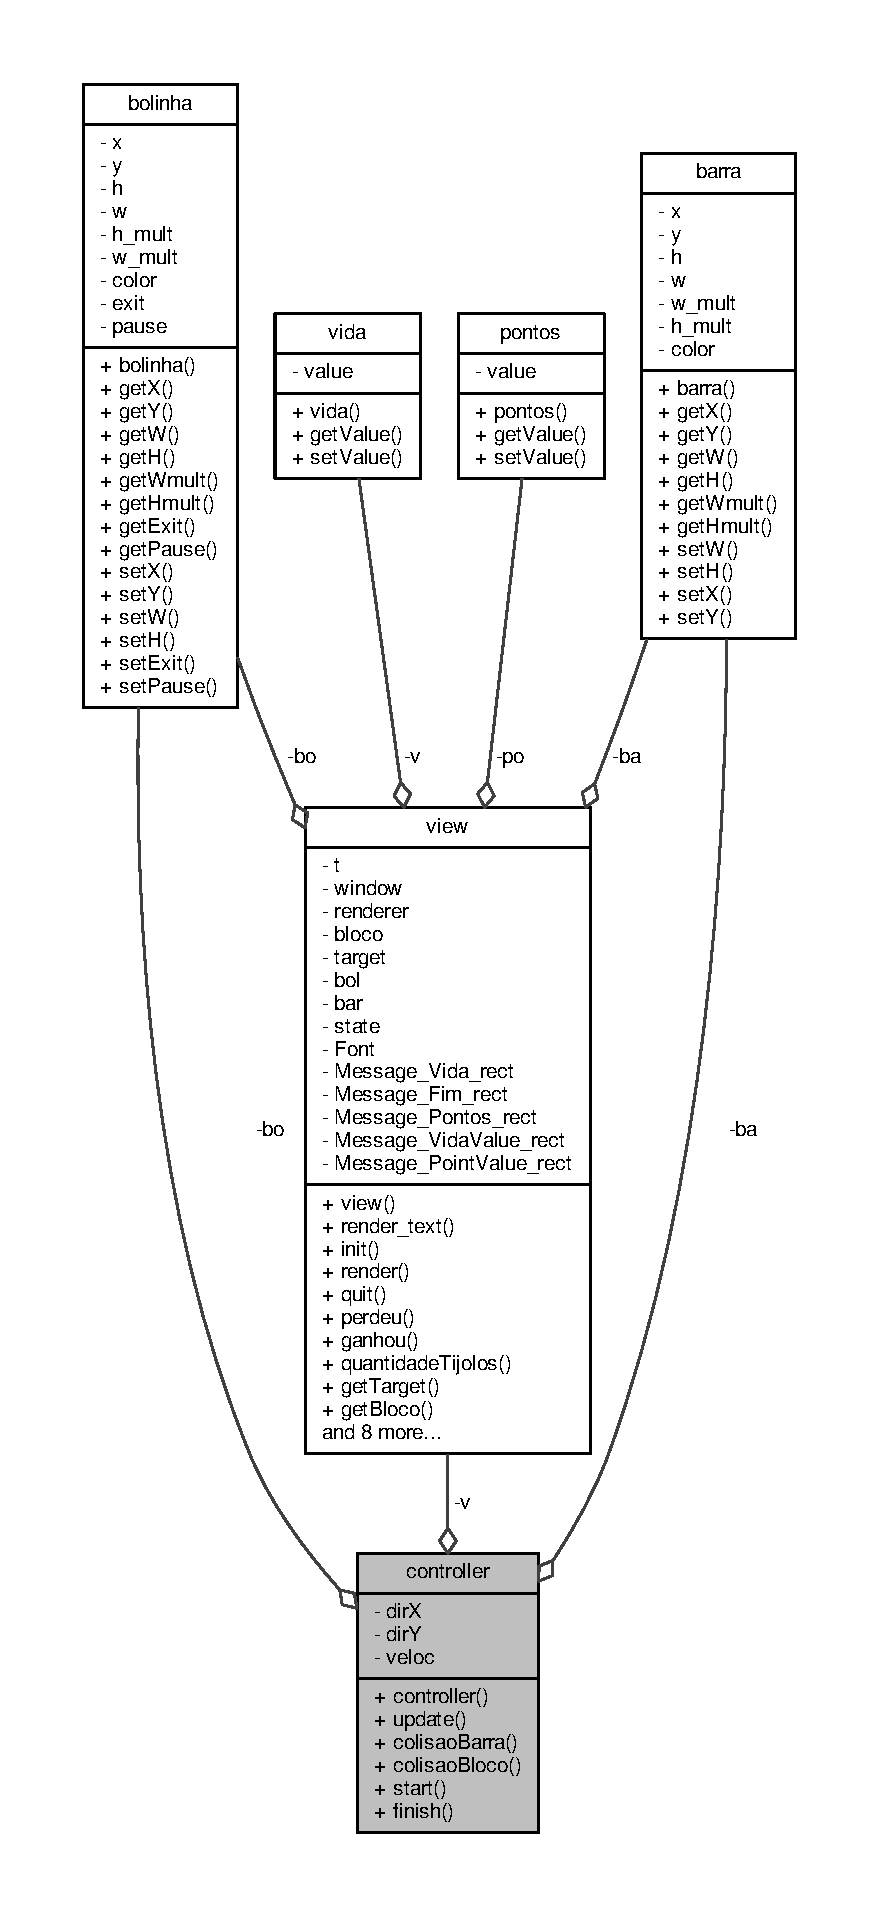
\includegraphics[height=550pt]{classcontroller__coll__graph}
\end{center}
\end{figure}
\subsection*{Public Member Functions}
\begin{DoxyCompactItemize}
\item 
\hyperlink{classcontroller_a5179368251d444a67542bf506ffa6b9c}{controller} (\hyperlink{classview}{view} \&v\+\_\+, \hyperlink{classbarra}{barra} $\ast$ba\+\_\+, \hyperlink{classbolinha}{bolinha} $\ast$bo\+\_\+)
\begin{DoxyCompactList}\small\item\em Construtor do controller. \end{DoxyCompactList}\item 
void \hyperlink{classcontroller_ac0373785a91924ce3d480c1c7dedbd99}{update} ()
\begin{DoxyCompactList}\small\item\em Metodo de acao. \end{DoxyCompactList}\item 
bool \hyperlink{classcontroller_aaaef2bd34f643183bcd6fad64bea1005}{colisao\+Barra} ()
\begin{DoxyCompactList}\small\item\em Colisao barra/bolinha. \end{DoxyCompactList}\item 
bool \hyperlink{classcontroller_ac227dd1b72111d1c6da3362d60aa25d6}{colisao\+Bloco} ()
\begin{DoxyCompactList}\small\item\em Colisao blocos/bolinha. \end{DoxyCompactList}\item 
void \hyperlink{classcontroller_a03872ff488ab704038e14226a8e031ea}{start} ()
\begin{DoxyCompactList}\small\item\em Inicia o jogo. \end{DoxyCompactList}\item 
bool \hyperlink{classcontroller_a993c5fe7272f0435b4018f4b5d1fc1cb}{finish} ()
\begin{DoxyCompactList}\small\item\em Finaliza o jogo. \end{DoxyCompactList}\end{DoxyCompactItemize}
\subsection*{Private Attributes}
\begin{DoxyCompactItemize}
\item 
\hyperlink{classview}{view} \& \hyperlink{classcontroller_a6ff845413a797ed4beff34d3cb6b7774}{v}
\item 
\hyperlink{classbarra}{barra} $\ast$ \hyperlink{classcontroller_af46499f5a9ef1afc0c95d899fb128aa1}{ba}
\item 
\hyperlink{classbolinha}{bolinha} $\ast$ \hyperlink{classcontroller_ae3e29aaa568c3d374b65416fd49649c5}{bo}
\item 
int \hyperlink{classcontroller_ab7bee2a38038001992ab877caccc1a47}{dirX} = 5
\item 
int \hyperlink{classcontroller_a136888a5f98296f5266a01330e2881e7}{dirY} = 5
\item 
int \hyperlink{classcontroller_ae1229353be5404b8decda1e8775292c4}{veloc} = 10
\end{DoxyCompactItemize}


\subsection{Detailed Description}
Classe para o controller. 

Esta é a classe para o controller. Ela faz o link entre os controles direcionais e a barra, tambem faz a movimentacao da bolinha, assim como sua colisao com as bordas da tela, barra e blocos. Faz tambem a destruicao do bloco e o reposicionamento da bolinha 

\subsection{Constructor \& Destructor Documentation}
\index{controller@{controller}!controller@{controller}}
\index{controller@{controller}!controller@{controller}}
\subsubsection[{\texorpdfstring{controller(view \&v\+\_\+, barra $\ast$ba\+\_\+, bolinha $\ast$bo\+\_\+)}{controller(view &v_, barra *ba_, bolinha *bo_)}}]{\setlength{\rightskip}{0pt plus 5cm}controller\+::controller (
\begin{DoxyParamCaption}
\item[{{\bf view} \&}]{v\+\_\+, }
\item[{{\bf barra} $\ast$}]{ba\+\_\+, }
\item[{{\bf bolinha} $\ast$}]{bo\+\_\+}
\end{DoxyParamCaption}
)\hspace{0.3cm}{\ttfamily [inline]}}\hypertarget{classcontroller_a5179368251d444a67542bf506ffa6b9c}{}\label{classcontroller_a5179368251d444a67542bf506ffa6b9c}


Construtor do controller. 

Recebe um view, uma barra e uma bolinha


\begin{DoxyParams}{Parameters}
{\em v\+\_\+} & um objeto view onde os objetos vao ser mostrados \\
\hline
{\em ba\+\_\+} & objeto barra \\
\hline
{\em bo\+\_\+} & objeto bolinha \\
\hline
\end{DoxyParams}


\subsection{Member Function Documentation}
\index{controller@{controller}!colisao\+Barra@{colisao\+Barra}}
\index{colisao\+Barra@{colisao\+Barra}!controller@{controller}}
\subsubsection[{\texorpdfstring{colisao\+Barra()}{colisaoBarra()}}]{\setlength{\rightskip}{0pt plus 5cm}bool controller\+::colisao\+Barra (
\begin{DoxyParamCaption}
{}
\end{DoxyParamCaption}
)}\hypertarget{classcontroller_aaaef2bd34f643183bcd6fad64bea1005}{}\label{classcontroller_aaaef2bd34f643183bcd6fad64bea1005}


Colisao barra/bolinha. 

checa a colisao entre a barra e a bolinha

\begin{DoxyReturn}{Returns}
retorna true caso haja colisao 
\end{DoxyReturn}
\index{controller@{controller}!colisao\+Bloco@{colisao\+Bloco}}
\index{colisao\+Bloco@{colisao\+Bloco}!controller@{controller}}
\subsubsection[{\texorpdfstring{colisao\+Bloco()}{colisaoBloco()}}]{\setlength{\rightskip}{0pt plus 5cm}bool controller\+::colisao\+Bloco (
\begin{DoxyParamCaption}
{}
\end{DoxyParamCaption}
)}\hypertarget{classcontroller_ac227dd1b72111d1c6da3362d60aa25d6}{}\label{classcontroller_ac227dd1b72111d1c6da3362d60aa25d6}


Colisao blocos/bolinha. 

checa a colisao entre a todos os blocos e a bolinha caso haja colisao, tira o bloco da visualizacao

\begin{DoxyReturn}{Returns}
retorna true caso haja colisao 
\end{DoxyReturn}
\index{controller@{controller}!finish@{finish}}
\index{finish@{finish}!controller@{controller}}
\subsubsection[{\texorpdfstring{finish()}{finish()}}]{\setlength{\rightskip}{0pt plus 5cm}bool controller\+::finish (
\begin{DoxyParamCaption}
{}
\end{DoxyParamCaption}
)}\hypertarget{classcontroller_a993c5fe7272f0435b4018f4b5d1fc1cb}{}\label{classcontroller_a993c5fe7272f0435b4018f4b5d1fc1cb}


Finaliza o jogo. 

checa se uma tecla previamente estabelecida foi pressionada, encerrando a execução e fechando o programa (Tecla Esc) \index{controller@{controller}!start@{start}}
\index{start@{start}!controller@{controller}}
\subsubsection[{\texorpdfstring{start()}{start()}}]{\setlength{\rightskip}{0pt plus 5cm}void controller\+::start (
\begin{DoxyParamCaption}
{}
\end{DoxyParamCaption}
)}\hypertarget{classcontroller_a03872ff488ab704038e14226a8e031ea}{}\label{classcontroller_a03872ff488ab704038e14226a8e031ea}


Inicia o jogo. 

checa se uma tecla previamente estabelecida foi pressionada, iniciando o movimento da bolinha (Tecla S) \index{controller@{controller}!update@{update}}
\index{update@{update}!controller@{controller}}
\subsubsection[{\texorpdfstring{update()}{update()}}]{\setlength{\rightskip}{0pt plus 5cm}void controller\+::update (
\begin{DoxyParamCaption}
{}
\end{DoxyParamCaption}
)}\hypertarget{classcontroller_ac0373785a91924ce3d480c1c7dedbd99}{}\label{classcontroller_ac0373785a91924ce3d480c1c7dedbd99}


Metodo de acao. 

serie de eventos que acontecem a cada ciclo de jogo 

\subsection{Member Data Documentation}
\index{controller@{controller}!ba@{ba}}
\index{ba@{ba}!controller@{controller}}
\subsubsection[{\texorpdfstring{ba}{ba}}]{\setlength{\rightskip}{0pt plus 5cm}{\bf barra}$\ast$ controller\+::ba\hspace{0.3cm}{\ttfamily [private]}}\hypertarget{classcontroller_af46499f5a9ef1afc0c95d899fb128aa1}{}\label{classcontroller_af46499f5a9ef1afc0c95d899fb128aa1}
barra (alocada previamente \index{controller@{controller}!bo@{bo}}
\index{bo@{bo}!controller@{controller}}
\subsubsection[{\texorpdfstring{bo}{bo}}]{\setlength{\rightskip}{0pt plus 5cm}{\bf bolinha}$\ast$ controller\+::bo\hspace{0.3cm}{\ttfamily [private]}}\hypertarget{classcontroller_ae3e29aaa568c3d374b65416fd49649c5}{}\label{classcontroller_ae3e29aaa568c3d374b65416fd49649c5}
bolinha (alocada previamente) \index{controller@{controller}!dirX@{dirX}}
\index{dirX@{dirX}!controller@{controller}}
\subsubsection[{\texorpdfstring{dirX}{dirX}}]{\setlength{\rightskip}{0pt plus 5cm}int controller\+::dirX = 5\hspace{0.3cm}{\ttfamily [private]}}\hypertarget{classcontroller_ab7bee2a38038001992ab877caccc1a47}{}\label{classcontroller_ab7bee2a38038001992ab877caccc1a47}
direcao de movimentacao da bolinha em X \index{controller@{controller}!dirY@{dirY}}
\index{dirY@{dirY}!controller@{controller}}
\subsubsection[{\texorpdfstring{dirY}{dirY}}]{\setlength{\rightskip}{0pt plus 5cm}int controller\+::dirY = 5\hspace{0.3cm}{\ttfamily [private]}}\hypertarget{classcontroller_a136888a5f98296f5266a01330e2881e7}{}\label{classcontroller_a136888a5f98296f5266a01330e2881e7}
direcao de movimentacao da bolinha em Y \index{controller@{controller}!v@{v}}
\index{v@{v}!controller@{controller}}
\subsubsection[{\texorpdfstring{v}{v}}]{\setlength{\rightskip}{0pt plus 5cm}{\bf view}\& controller\+::v\hspace{0.3cm}{\ttfamily [private]}}\hypertarget{classcontroller_a6ff845413a797ed4beff34d3cb6b7774}{}\label{classcontroller_a6ff845413a797ed4beff34d3cb6b7774}
view (alocado previamente) \index{controller@{controller}!veloc@{veloc}}
\index{veloc@{veloc}!controller@{controller}}
\subsubsection[{\texorpdfstring{veloc}{veloc}}]{\setlength{\rightskip}{0pt plus 5cm}int controller\+::veloc = 10\hspace{0.3cm}{\ttfamily [private]}}\hypertarget{classcontroller_ae1229353be5404b8decda1e8775292c4}{}\label{classcontroller_ae1229353be5404b8decda1e8775292c4}
velocidade de movimentacao da bolinha 

The documentation for this class was generated from the following files\+:\begin{DoxyCompactItemize}
\item 
include/\hyperlink{controller_8h}{controller.\+h}\item 
src/controller/\hyperlink{controller_8cpp}{controller.\+cpp}\end{DoxyCompactItemize}

\hypertarget{classpontos}{}\section{pontos Class Reference}
\label{classpontos}\index{pontos@{pontos}}


Classe para os pontos.  




{\ttfamily \#include $<$pontos.\+h$>$}



Collaboration diagram for pontos\+:
\nopagebreak
\begin{figure}[H]
\begin{center}
\leavevmode
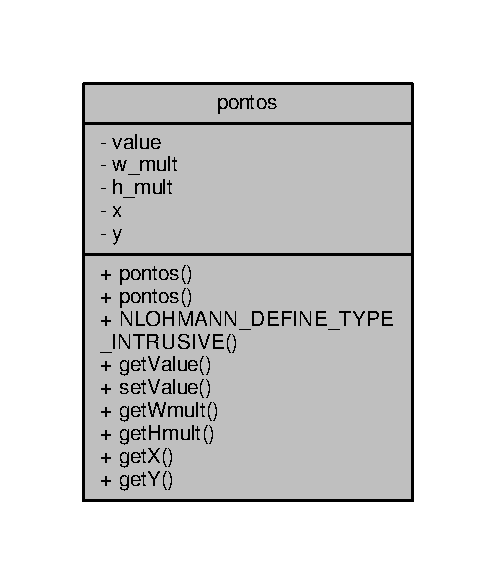
\includegraphics[width=238pt]{classpontos__coll__graph}
\end{center}
\end{figure}
\subsection*{Public Member Functions}
\begin{DoxyCompactItemize}
\item 
\hyperlink{classpontos_ac2c939539723b5f20054239c0c78ef59}{pontos} (int value\+\_\+)
\item 
\hyperlink{classpontos_aa12034740983c0d4577f45b77d554614}{pontos} ()
\item 
\hyperlink{classpontos_affd7bca089c5a4b687b4cc4faa0ab2ef}{N\+L\+O\+H\+M\+A\+N\+N\+\_\+\+D\+E\+F\+I\+N\+E\+\_\+\+T\+Y\+P\+E\+\_\+\+I\+N\+T\+R\+U\+S\+I\+VE} (\hyperlink{classpontos}{pontos}, \hyperlink{classpontos_a776f5643630f9aec273380a31d0e6e47}{value})
\item 
int \hyperlink{classpontos_a928ec19b58787b0dec93b801a9670070}{get\+Value} ()
\item 
void \hyperlink{classpontos_a75f82ace742aedeb18c05e4130f45951}{set\+Value} (int value\+\_\+)
\item 
float \hyperlink{classpontos_a512205d058f86aa9add643b8e3eb7b37}{get\+Wmult} ()
\item 
float \hyperlink{classpontos_a272201de7460bc20bb297cc45cf09601}{get\+Hmult} ()
\item 
int \hyperlink{classpontos_a9ade2e54b1349e7dfb3a67ced58ab198}{getX} ()
\item 
int \hyperlink{classpontos_add5e95747077e412c6cb3246213427df}{getY} ()
\end{DoxyCompactItemize}
\subsection*{Private Attributes}
\begin{DoxyCompactItemize}
\item 
int \hyperlink{classpontos_a776f5643630f9aec273380a31d0e6e47}{value}
\item 
float \hyperlink{classpontos_a5809900ae2d67c4f1188e4fa7e1e5d85}{w\+\_\+mult} =2
\item 
float \hyperlink{classpontos_a047ccb35d9d6ec355dd75a7651186a2a}{h\+\_\+mult} =0.\+5
\item 
int \hyperlink{classpontos_a8801f4bd9a7391355b70bb23642cc5da}{x} = 5.\+5
\item 
int \hyperlink{classpontos_ac046437304ec67cf1e820775bb74e52e}{y} = 0.\+7
\end{DoxyCompactItemize}


\subsection{Detailed Description}
Classe para os pontos. 

Classe utilizada para armazenar os pontos do jogador. 

\subsection{Constructor \& Destructor Documentation}
\index{pontos@{pontos}!pontos@{pontos}}
\index{pontos@{pontos}!pontos@{pontos}}
\subsubsection[{\texorpdfstring{pontos(int value\+\_\+)}{pontos(int value_)}}]{\setlength{\rightskip}{0pt plus 5cm}pontos\+::pontos (
\begin{DoxyParamCaption}
\item[{int}]{value\+\_\+}
\end{DoxyParamCaption}
)}\hypertarget{classpontos_ac2c939539723b5f20054239c0c78ef59}{}\label{classpontos_ac2c939539723b5f20054239c0c78ef59}
\index{pontos@{pontos}!pontos@{pontos}}
\index{pontos@{pontos}!pontos@{pontos}}
\subsubsection[{\texorpdfstring{pontos()}{pontos()}}]{\setlength{\rightskip}{0pt plus 5cm}pontos\+::pontos (
\begin{DoxyParamCaption}
{}
\end{DoxyParamCaption}
)}\hypertarget{classpontos_aa12034740983c0d4577f45b77d554614}{}\label{classpontos_aa12034740983c0d4577f45b77d554614}


\subsection{Member Function Documentation}
\index{pontos@{pontos}!get\+Hmult@{get\+Hmult}}
\index{get\+Hmult@{get\+Hmult}!pontos@{pontos}}
\subsubsection[{\texorpdfstring{get\+Hmult()}{getHmult()}}]{\setlength{\rightskip}{0pt plus 5cm}float pontos\+::get\+Hmult (
\begin{DoxyParamCaption}
{}
\end{DoxyParamCaption}
)}\hypertarget{classpontos_a272201de7460bc20bb297cc45cf09601}{}\label{classpontos_a272201de7460bc20bb297cc45cf09601}
\index{pontos@{pontos}!get\+Value@{get\+Value}}
\index{get\+Value@{get\+Value}!pontos@{pontos}}
\subsubsection[{\texorpdfstring{get\+Value()}{getValue()}}]{\setlength{\rightskip}{0pt plus 5cm}int pontos\+::get\+Value (
\begin{DoxyParamCaption}
{}
\end{DoxyParamCaption}
)}\hypertarget{classpontos_a928ec19b58787b0dec93b801a9670070}{}\label{classpontos_a928ec19b58787b0dec93b801a9670070}
\index{pontos@{pontos}!get\+Wmult@{get\+Wmult}}
\index{get\+Wmult@{get\+Wmult}!pontos@{pontos}}
\subsubsection[{\texorpdfstring{get\+Wmult()}{getWmult()}}]{\setlength{\rightskip}{0pt plus 5cm}float pontos\+::get\+Wmult (
\begin{DoxyParamCaption}
{}
\end{DoxyParamCaption}
)}\hypertarget{classpontos_a512205d058f86aa9add643b8e3eb7b37}{}\label{classpontos_a512205d058f86aa9add643b8e3eb7b37}
\index{pontos@{pontos}!getX@{getX}}
\index{getX@{getX}!pontos@{pontos}}
\subsubsection[{\texorpdfstring{get\+X()}{getX()}}]{\setlength{\rightskip}{0pt plus 5cm}int pontos\+::getX (
\begin{DoxyParamCaption}
{}
\end{DoxyParamCaption}
)}\hypertarget{classpontos_a9ade2e54b1349e7dfb3a67ced58ab198}{}\label{classpontos_a9ade2e54b1349e7dfb3a67ced58ab198}
\index{pontos@{pontos}!getY@{getY}}
\index{getY@{getY}!pontos@{pontos}}
\subsubsection[{\texorpdfstring{get\+Y()}{getY()}}]{\setlength{\rightskip}{0pt plus 5cm}int pontos\+::getY (
\begin{DoxyParamCaption}
{}
\end{DoxyParamCaption}
)}\hypertarget{classpontos_add5e95747077e412c6cb3246213427df}{}\label{classpontos_add5e95747077e412c6cb3246213427df}
\index{pontos@{pontos}!N\+L\+O\+H\+M\+A\+N\+N\+\_\+\+D\+E\+F\+I\+N\+E\+\_\+\+T\+Y\+P\+E\+\_\+\+I\+N\+T\+R\+U\+S\+I\+VE@{N\+L\+O\+H\+M\+A\+N\+N\+\_\+\+D\+E\+F\+I\+N\+E\+\_\+\+T\+Y\+P\+E\+\_\+\+I\+N\+T\+R\+U\+S\+I\+VE}}
\index{N\+L\+O\+H\+M\+A\+N\+N\+\_\+\+D\+E\+F\+I\+N\+E\+\_\+\+T\+Y\+P\+E\+\_\+\+I\+N\+T\+R\+U\+S\+I\+VE@{N\+L\+O\+H\+M\+A\+N\+N\+\_\+\+D\+E\+F\+I\+N\+E\+\_\+\+T\+Y\+P\+E\+\_\+\+I\+N\+T\+R\+U\+S\+I\+VE}!pontos@{pontos}}
\subsubsection[{\texorpdfstring{N\+L\+O\+H\+M\+A\+N\+N\+\_\+\+D\+E\+F\+I\+N\+E\+\_\+\+T\+Y\+P\+E\+\_\+\+I\+N\+T\+R\+U\+S\+I\+V\+E(pontos, value)}{NLOHMANN_DEFINE_TYPE_INTRUSIVE(pontos, value)}}]{\setlength{\rightskip}{0pt plus 5cm}pontos\+::\+N\+L\+O\+H\+M\+A\+N\+N\+\_\+\+D\+E\+F\+I\+N\+E\+\_\+\+T\+Y\+P\+E\+\_\+\+I\+N\+T\+R\+U\+S\+I\+VE (
\begin{DoxyParamCaption}
\item[{{\bf pontos}}]{, }
\item[{{\bf value}}]{}
\end{DoxyParamCaption}
)}\hypertarget{classpontos_affd7bca089c5a4b687b4cc4faa0ab2ef}{}\label{classpontos_affd7bca089c5a4b687b4cc4faa0ab2ef}
\index{pontos@{pontos}!set\+Value@{set\+Value}}
\index{set\+Value@{set\+Value}!pontos@{pontos}}
\subsubsection[{\texorpdfstring{set\+Value(int value\+\_\+)}{setValue(int value_)}}]{\setlength{\rightskip}{0pt plus 5cm}void pontos\+::set\+Value (
\begin{DoxyParamCaption}
\item[{int}]{value\+\_\+}
\end{DoxyParamCaption}
)}\hypertarget{classpontos_a75f82ace742aedeb18c05e4130f45951}{}\label{classpontos_a75f82ace742aedeb18c05e4130f45951}


\subsection{Member Data Documentation}
\index{pontos@{pontos}!h\+\_\+mult@{h\+\_\+mult}}
\index{h\+\_\+mult@{h\+\_\+mult}!pontos@{pontos}}
\subsubsection[{\texorpdfstring{h\+\_\+mult}{h_mult}}]{\setlength{\rightskip}{0pt plus 5cm}float pontos\+::h\+\_\+mult =0.\+5\hspace{0.3cm}{\ttfamily [private]}}\hypertarget{classpontos_a047ccb35d9d6ec355dd75a7651186a2a}{}\label{classpontos_a047ccb35d9d6ec355dd75a7651186a2a}
\index{pontos@{pontos}!value@{value}}
\index{value@{value}!pontos@{pontos}}
\subsubsection[{\texorpdfstring{value}{value}}]{\setlength{\rightskip}{0pt plus 5cm}int pontos\+::value\hspace{0.3cm}{\ttfamily [private]}}\hypertarget{classpontos_a776f5643630f9aec273380a31d0e6e47}{}\label{classpontos_a776f5643630f9aec273380a31d0e6e47}
quantidade de pontos \index{pontos@{pontos}!w\+\_\+mult@{w\+\_\+mult}}
\index{w\+\_\+mult@{w\+\_\+mult}!pontos@{pontos}}
\subsubsection[{\texorpdfstring{w\+\_\+mult}{w_mult}}]{\setlength{\rightskip}{0pt plus 5cm}float pontos\+::w\+\_\+mult =2\hspace{0.3cm}{\ttfamily [private]}}\hypertarget{classpontos_a5809900ae2d67c4f1188e4fa7e1e5d85}{}\label{classpontos_a5809900ae2d67c4f1188e4fa7e1e5d85}
\index{pontos@{pontos}!x@{x}}
\index{x@{x}!pontos@{pontos}}
\subsubsection[{\texorpdfstring{x}{x}}]{\setlength{\rightskip}{0pt plus 5cm}int pontos\+::x = 5.\+5\hspace{0.3cm}{\ttfamily [private]}}\hypertarget{classpontos_a8801f4bd9a7391355b70bb23642cc5da}{}\label{classpontos_a8801f4bd9a7391355b70bb23642cc5da}
\index{pontos@{pontos}!y@{y}}
\index{y@{y}!pontos@{pontos}}
\subsubsection[{\texorpdfstring{y}{y}}]{\setlength{\rightskip}{0pt plus 5cm}int pontos\+::y = 0.\+7\hspace{0.3cm}{\ttfamily [private]}}\hypertarget{classpontos_ac046437304ec67cf1e820775bb74e52e}{}\label{classpontos_ac046437304ec67cf1e820775bb74e52e}


The documentation for this class was generated from the following files\+:\begin{DoxyCompactItemize}
\item 
include/\hyperlink{pontos_8h}{pontos.\+h}\item 
src/model/\hyperlink{pontos_8cpp}{pontos.\+cpp}\end{DoxyCompactItemize}

\hypertarget{classtijolo}{}\section{tijolo Class Reference}
\label{classtijolo}\index{tijolo@{tijolo}}


Classe para os pontos.  




{\ttfamily \#include $<$tijolo.\+h$>$}



Collaboration diagram for tijolo\+:
\nopagebreak
\begin{figure}[H]
\begin{center}
\leavevmode
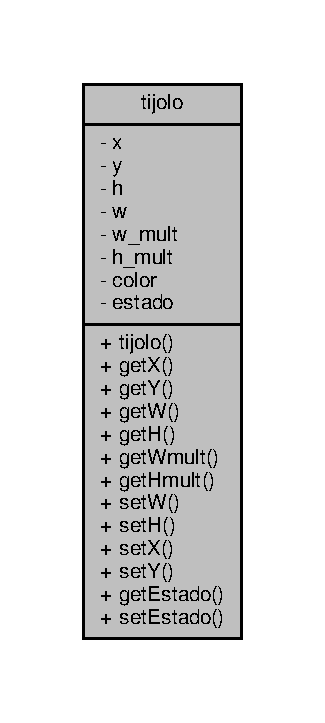
\includegraphics[width=238pt]{classtijolo__coll__graph}
\end{center}
\end{figure}
\subsection*{Public Member Functions}
\begin{DoxyCompactItemize}
\item 
\hyperlink{classtijolo_addedf3e33eb8134576997ef0c29d918a}{N\+L\+O\+H\+M\+A\+N\+N\+\_\+\+D\+E\+F\+I\+N\+E\+\_\+\+T\+Y\+P\+E\+\_\+\+I\+N\+T\+R\+U\+S\+I\+VE} (\hyperlink{classtijolo}{tijolo}, \hyperlink{classtijolo_acd39a70440853d5f019378ab501fb688}{x}, \hyperlink{classtijolo_a3089987dab8db697303f88bd59c0989f}{y}, \hyperlink{classtijolo_a11e0c9ba0ab09baad2622ba49de44f8a}{w}, \hyperlink{classtijolo_ad96e30c66b061844a9a3f3b60d4bfcf2}{h}, \hyperlink{classtijolo_a14a93338f6c68097ba6e8afe18a32f60}{x\+\_\+param}, \hyperlink{classtijolo_ab4b4106e1ff29da211d56df195bb919a}{y\+\_\+param})
\item 
\hyperlink{classtijolo_a1575297d58f55111b16bfde06d7fcf14}{tijolo} (int x\+\_\+, int y\+\_\+)
\item 
\hyperlink{classtijolo_ab85f837336b5668d8db4a1119034493d}{tijolo} ()
\item 
int \hyperlink{classtijolo_ab3179398dd6fe44db34eb23556ccd029}{getX} ()
\item 
int \hyperlink{classtijolo_ad5d4edc964d42505990ab3c0e739f175}{getY} ()
\item 
int \hyperlink{classtijolo_a940e6fd9de3320009415b3ee5d9a89ea}{getW} ()
\item 
int \hyperlink{classtijolo_ad742e39614eec9ad0ac8d1e386fee696}{getH} ()
\item 
float \hyperlink{classtijolo_acb8367de6befb88b131e3cb8dd4be70f}{get\+Wmult} ()
\item 
float \hyperlink{classtijolo_ac3b530ef0293d8d5973fa2087c7ea9b9}{get\+Hmult} ()
\item 
float \hyperlink{classtijolo_aa2ec8732cec3b95a13bb3cbdbd533011}{get\+Xparam} ()
\item 
float \hyperlink{classtijolo_acee30dfee179445d4d42d815e781d96f}{get\+Yparam} ()
\item 
void \hyperlink{classtijolo_a962fd6769fcf78defe69bb77cc881172}{set\+Xparam} (float x\+\_\+param\+\_\+)
\item 
void \hyperlink{classtijolo_ad5d5063df5809d7b8db5a8c55649f1cc}{set\+Yparam} (float y\+\_\+param\+\_\+)
\item 
void \hyperlink{classtijolo_a6f5eed3413774d0e4d9ee7505a0a68e3}{setW} (int w\+\_\+)
\item 
void \hyperlink{classtijolo_ac15a68731bbf0019493a54ab0bccb04d}{setH} (int h\+\_\+)
\item 
void \hyperlink{classtijolo_afce75411c77a0f53037c33e7a3321d4b}{setX} (int x\+\_\+)
\item 
void \hyperlink{classtijolo_ac1d41f557b4d2170dc4fd4ff53a78c13}{setY} (int y\+\_\+)
\end{DoxyCompactItemize}
\subsection*{Private Attributes}
\begin{DoxyCompactItemize}
\item 
int \hyperlink{classtijolo_acd39a70440853d5f019378ab501fb688}{x}
\item 
int \hyperlink{classtijolo_a3089987dab8db697303f88bd59c0989f}{y}
\item 
int \hyperlink{classtijolo_ad96e30c66b061844a9a3f3b60d4bfcf2}{h}
\item 
int \hyperlink{classtijolo_a11e0c9ba0ab09baad2622ba49de44f8a}{w}
\item 
float \hyperlink{classtijolo_a14a93338f6c68097ba6e8afe18a32f60}{x\+\_\+param}
\item 
float \hyperlink{classtijolo_ab4b4106e1ff29da211d56df195bb919a}{y\+\_\+param}
\item 
float \hyperlink{classtijolo_a541d86c88882bb3be2199b10f840777c}{w\+\_\+mult} =1
\item 
float \hyperlink{classtijolo_a4c6684dc3837ed50b9111ccbd4e95d23}{h\+\_\+mult} =0.\+5
\item 
int \hyperlink{classtijolo_aad4f2b8b44ee1df886b58a60b7a9f653}{color}
\end{DoxyCompactItemize}


\subsection{Detailed Description}
Classe para os pontos. 

Classe utilizada para os tijolos. 

\subsection{Constructor \& Destructor Documentation}
\index{tijolo@{tijolo}!tijolo@{tijolo}}
\index{tijolo@{tijolo}!tijolo@{tijolo}}
\subsubsection[{\texorpdfstring{tijolo(int x\+\_\+, int y\+\_\+)}{tijolo(int x_, int y_)}}]{\setlength{\rightskip}{0pt plus 5cm}tijolo\+::tijolo (
\begin{DoxyParamCaption}
\item[{int}]{x\+\_\+, }
\item[{int}]{y\+\_\+}
\end{DoxyParamCaption}
)}\hypertarget{classtijolo_a1575297d58f55111b16bfde06d7fcf14}{}\label{classtijolo_a1575297d58f55111b16bfde06d7fcf14}
\index{tijolo@{tijolo}!tijolo@{tijolo}}
\index{tijolo@{tijolo}!tijolo@{tijolo}}
\subsubsection[{\texorpdfstring{tijolo()}{tijolo()}}]{\setlength{\rightskip}{0pt plus 5cm}tijolo\+::tijolo (
\begin{DoxyParamCaption}
{}
\end{DoxyParamCaption}
)}\hypertarget{classtijolo_ab85f837336b5668d8db4a1119034493d}{}\label{classtijolo_ab85f837336b5668d8db4a1119034493d}


\subsection{Member Function Documentation}
\index{tijolo@{tijolo}!getH@{getH}}
\index{getH@{getH}!tijolo@{tijolo}}
\subsubsection[{\texorpdfstring{get\+H()}{getH()}}]{\setlength{\rightskip}{0pt plus 5cm}int tijolo\+::getH (
\begin{DoxyParamCaption}
{}
\end{DoxyParamCaption}
)}\hypertarget{classtijolo_ad742e39614eec9ad0ac8d1e386fee696}{}\label{classtijolo_ad742e39614eec9ad0ac8d1e386fee696}
\index{tijolo@{tijolo}!get\+Hmult@{get\+Hmult}}
\index{get\+Hmult@{get\+Hmult}!tijolo@{tijolo}}
\subsubsection[{\texorpdfstring{get\+Hmult()}{getHmult()}}]{\setlength{\rightskip}{0pt plus 5cm}float tijolo\+::get\+Hmult (
\begin{DoxyParamCaption}
{}
\end{DoxyParamCaption}
)}\hypertarget{classtijolo_ac3b530ef0293d8d5973fa2087c7ea9b9}{}\label{classtijolo_ac3b530ef0293d8d5973fa2087c7ea9b9}
\index{tijolo@{tijolo}!getW@{getW}}
\index{getW@{getW}!tijolo@{tijolo}}
\subsubsection[{\texorpdfstring{get\+W()}{getW()}}]{\setlength{\rightskip}{0pt plus 5cm}int tijolo\+::getW (
\begin{DoxyParamCaption}
{}
\end{DoxyParamCaption}
)}\hypertarget{classtijolo_a940e6fd9de3320009415b3ee5d9a89ea}{}\label{classtijolo_a940e6fd9de3320009415b3ee5d9a89ea}
\index{tijolo@{tijolo}!get\+Wmult@{get\+Wmult}}
\index{get\+Wmult@{get\+Wmult}!tijolo@{tijolo}}
\subsubsection[{\texorpdfstring{get\+Wmult()}{getWmult()}}]{\setlength{\rightskip}{0pt plus 5cm}float tijolo\+::get\+Wmult (
\begin{DoxyParamCaption}
{}
\end{DoxyParamCaption}
)}\hypertarget{classtijolo_acb8367de6befb88b131e3cb8dd4be70f}{}\label{classtijolo_acb8367de6befb88b131e3cb8dd4be70f}
\index{tijolo@{tijolo}!getX@{getX}}
\index{getX@{getX}!tijolo@{tijolo}}
\subsubsection[{\texorpdfstring{get\+X()}{getX()}}]{\setlength{\rightskip}{0pt plus 5cm}int tijolo\+::getX (
\begin{DoxyParamCaption}
{}
\end{DoxyParamCaption}
)}\hypertarget{classtijolo_ab3179398dd6fe44db34eb23556ccd029}{}\label{classtijolo_ab3179398dd6fe44db34eb23556ccd029}
\index{tijolo@{tijolo}!get\+Xparam@{get\+Xparam}}
\index{get\+Xparam@{get\+Xparam}!tijolo@{tijolo}}
\subsubsection[{\texorpdfstring{get\+Xparam()}{getXparam()}}]{\setlength{\rightskip}{0pt plus 5cm}float tijolo\+::get\+Xparam (
\begin{DoxyParamCaption}
{}
\end{DoxyParamCaption}
)}\hypertarget{classtijolo_aa2ec8732cec3b95a13bb3cbdbd533011}{}\label{classtijolo_aa2ec8732cec3b95a13bb3cbdbd533011}
\index{tijolo@{tijolo}!getY@{getY}}
\index{getY@{getY}!tijolo@{tijolo}}
\subsubsection[{\texorpdfstring{get\+Y()}{getY()}}]{\setlength{\rightskip}{0pt plus 5cm}int tijolo\+::getY (
\begin{DoxyParamCaption}
{}
\end{DoxyParamCaption}
)}\hypertarget{classtijolo_ad5d4edc964d42505990ab3c0e739f175}{}\label{classtijolo_ad5d4edc964d42505990ab3c0e739f175}
\index{tijolo@{tijolo}!get\+Yparam@{get\+Yparam}}
\index{get\+Yparam@{get\+Yparam}!tijolo@{tijolo}}
\subsubsection[{\texorpdfstring{get\+Yparam()}{getYparam()}}]{\setlength{\rightskip}{0pt plus 5cm}float tijolo\+::get\+Yparam (
\begin{DoxyParamCaption}
{}
\end{DoxyParamCaption}
)}\hypertarget{classtijolo_acee30dfee179445d4d42d815e781d96f}{}\label{classtijolo_acee30dfee179445d4d42d815e781d96f}
\index{tijolo@{tijolo}!N\+L\+O\+H\+M\+A\+N\+N\+\_\+\+D\+E\+F\+I\+N\+E\+\_\+\+T\+Y\+P\+E\+\_\+\+I\+N\+T\+R\+U\+S\+I\+VE@{N\+L\+O\+H\+M\+A\+N\+N\+\_\+\+D\+E\+F\+I\+N\+E\+\_\+\+T\+Y\+P\+E\+\_\+\+I\+N\+T\+R\+U\+S\+I\+VE}}
\index{N\+L\+O\+H\+M\+A\+N\+N\+\_\+\+D\+E\+F\+I\+N\+E\+\_\+\+T\+Y\+P\+E\+\_\+\+I\+N\+T\+R\+U\+S\+I\+VE@{N\+L\+O\+H\+M\+A\+N\+N\+\_\+\+D\+E\+F\+I\+N\+E\+\_\+\+T\+Y\+P\+E\+\_\+\+I\+N\+T\+R\+U\+S\+I\+VE}!tijolo@{tijolo}}
\subsubsection[{\texorpdfstring{N\+L\+O\+H\+M\+A\+N\+N\+\_\+\+D\+E\+F\+I\+N\+E\+\_\+\+T\+Y\+P\+E\+\_\+\+I\+N\+T\+R\+U\+S\+I\+V\+E(tijolo, x, y, w, h, x\+\_\+param, y\+\_\+param)}{NLOHMANN_DEFINE_TYPE_INTRUSIVE(tijolo, x, y, w, h, x_param, y_param)}}]{\setlength{\rightskip}{0pt plus 5cm}tijolo\+::\+N\+L\+O\+H\+M\+A\+N\+N\+\_\+\+D\+E\+F\+I\+N\+E\+\_\+\+T\+Y\+P\+E\+\_\+\+I\+N\+T\+R\+U\+S\+I\+VE (
\begin{DoxyParamCaption}
\item[{{\bf tijolo}}]{, }
\item[{{\bf x}}]{, }
\item[{{\bf y}}]{, }
\item[{{\bf w}}]{, }
\item[{{\bf h}}]{, }
\item[{{\bf x\+\_\+param}}]{, }
\item[{{\bf y\+\_\+param}}]{}
\end{DoxyParamCaption}
)}\hypertarget{classtijolo_addedf3e33eb8134576997ef0c29d918a}{}\label{classtijolo_addedf3e33eb8134576997ef0c29d918a}
\index{tijolo@{tijolo}!setH@{setH}}
\index{setH@{setH}!tijolo@{tijolo}}
\subsubsection[{\texorpdfstring{set\+H(int h\+\_\+)}{setH(int h_)}}]{\setlength{\rightskip}{0pt plus 5cm}void tijolo\+::setH (
\begin{DoxyParamCaption}
\item[{int}]{h\+\_\+}
\end{DoxyParamCaption}
)}\hypertarget{classtijolo_ac15a68731bbf0019493a54ab0bccb04d}{}\label{classtijolo_ac15a68731bbf0019493a54ab0bccb04d}
\index{tijolo@{tijolo}!setW@{setW}}
\index{setW@{setW}!tijolo@{tijolo}}
\subsubsection[{\texorpdfstring{set\+W(int w\+\_\+)}{setW(int w_)}}]{\setlength{\rightskip}{0pt plus 5cm}void tijolo\+::setW (
\begin{DoxyParamCaption}
\item[{int}]{w\+\_\+}
\end{DoxyParamCaption}
)}\hypertarget{classtijolo_a6f5eed3413774d0e4d9ee7505a0a68e3}{}\label{classtijolo_a6f5eed3413774d0e4d9ee7505a0a68e3}
\index{tijolo@{tijolo}!setX@{setX}}
\index{setX@{setX}!tijolo@{tijolo}}
\subsubsection[{\texorpdfstring{set\+X(int x\+\_\+)}{setX(int x_)}}]{\setlength{\rightskip}{0pt plus 5cm}void tijolo\+::setX (
\begin{DoxyParamCaption}
\item[{int}]{x\+\_\+}
\end{DoxyParamCaption}
)}\hypertarget{classtijolo_afce75411c77a0f53037c33e7a3321d4b}{}\label{classtijolo_afce75411c77a0f53037c33e7a3321d4b}
\index{tijolo@{tijolo}!set\+Xparam@{set\+Xparam}}
\index{set\+Xparam@{set\+Xparam}!tijolo@{tijolo}}
\subsubsection[{\texorpdfstring{set\+Xparam(float x\+\_\+param\+\_\+)}{setXparam(float x_param_)}}]{\setlength{\rightskip}{0pt plus 5cm}void tijolo\+::set\+Xparam (
\begin{DoxyParamCaption}
\item[{float}]{x\+\_\+param\+\_\+}
\end{DoxyParamCaption}
)}\hypertarget{classtijolo_a962fd6769fcf78defe69bb77cc881172}{}\label{classtijolo_a962fd6769fcf78defe69bb77cc881172}
\index{tijolo@{tijolo}!setY@{setY}}
\index{setY@{setY}!tijolo@{tijolo}}
\subsubsection[{\texorpdfstring{set\+Y(int y\+\_\+)}{setY(int y_)}}]{\setlength{\rightskip}{0pt plus 5cm}void tijolo\+::setY (
\begin{DoxyParamCaption}
\item[{int}]{y\+\_\+}
\end{DoxyParamCaption}
)}\hypertarget{classtijolo_ac1d41f557b4d2170dc4fd4ff53a78c13}{}\label{classtijolo_ac1d41f557b4d2170dc4fd4ff53a78c13}
\index{tijolo@{tijolo}!set\+Yparam@{set\+Yparam}}
\index{set\+Yparam@{set\+Yparam}!tijolo@{tijolo}}
\subsubsection[{\texorpdfstring{set\+Yparam(float y\+\_\+param\+\_\+)}{setYparam(float y_param_)}}]{\setlength{\rightskip}{0pt plus 5cm}void tijolo\+::set\+Yparam (
\begin{DoxyParamCaption}
\item[{float}]{y\+\_\+param\+\_\+}
\end{DoxyParamCaption}
)}\hypertarget{classtijolo_ad5d5063df5809d7b8db5a8c55649f1cc}{}\label{classtijolo_ad5d5063df5809d7b8db5a8c55649f1cc}


\subsection{Member Data Documentation}
\index{tijolo@{tijolo}!color@{color}}
\index{color@{color}!tijolo@{tijolo}}
\subsubsection[{\texorpdfstring{color}{color}}]{\setlength{\rightskip}{0pt plus 5cm}int tijolo\+::color\hspace{0.3cm}{\ttfamily [private]}}\hypertarget{classtijolo_aad4f2b8b44ee1df886b58a60b7a9f653}{}\label{classtijolo_aad4f2b8b44ee1df886b58a60b7a9f653}
Cor da barra \index{tijolo@{tijolo}!h@{h}}
\index{h@{h}!tijolo@{tijolo}}
\subsubsection[{\texorpdfstring{h}{h}}]{\setlength{\rightskip}{0pt plus 5cm}int tijolo\+::h\hspace{0.3cm}{\ttfamily [private]}}\hypertarget{classtijolo_ad96e30c66b061844a9a3f3b60d4bfcf2}{}\label{classtijolo_ad96e30c66b061844a9a3f3b60d4bfcf2}
\index{tijolo@{tijolo}!h\+\_\+mult@{h\+\_\+mult}}
\index{h\+\_\+mult@{h\+\_\+mult}!tijolo@{tijolo}}
\subsubsection[{\texorpdfstring{h\+\_\+mult}{h_mult}}]{\setlength{\rightskip}{0pt plus 5cm}float tijolo\+::h\+\_\+mult =0.\+5\hspace{0.3cm}{\ttfamily [private]}}\hypertarget{classtijolo_a4c6684dc3837ed50b9111ccbd4e95d23}{}\label{classtijolo_a4c6684dc3837ed50b9111ccbd4e95d23}
Fator de multiplicacao para visualizacao \index{tijolo@{tijolo}!w@{w}}
\index{w@{w}!tijolo@{tijolo}}
\subsubsection[{\texorpdfstring{w}{w}}]{\setlength{\rightskip}{0pt plus 5cm}int tijolo\+::w\hspace{0.3cm}{\ttfamily [private]}}\hypertarget{classtijolo_a11e0c9ba0ab09baad2622ba49de44f8a}{}\label{classtijolo_a11e0c9ba0ab09baad2622ba49de44f8a}
Variaveis de dimensao \index{tijolo@{tijolo}!w\+\_\+mult@{w\+\_\+mult}}
\index{w\+\_\+mult@{w\+\_\+mult}!tijolo@{tijolo}}
\subsubsection[{\texorpdfstring{w\+\_\+mult}{w_mult}}]{\setlength{\rightskip}{0pt plus 5cm}float tijolo\+::w\+\_\+mult =1\hspace{0.3cm}{\ttfamily [private]}}\hypertarget{classtijolo_a541d86c88882bb3be2199b10f840777c}{}\label{classtijolo_a541d86c88882bb3be2199b10f840777c}
\index{tijolo@{tijolo}!x@{x}}
\index{x@{x}!tijolo@{tijolo}}
\subsubsection[{\texorpdfstring{x}{x}}]{\setlength{\rightskip}{0pt plus 5cm}int tijolo\+::x\hspace{0.3cm}{\ttfamily [private]}}\hypertarget{classtijolo_acd39a70440853d5f019378ab501fb688}{}\label{classtijolo_acd39a70440853d5f019378ab501fb688}
\index{tijolo@{tijolo}!x\+\_\+param@{x\+\_\+param}}
\index{x\+\_\+param@{x\+\_\+param}!tijolo@{tijolo}}
\subsubsection[{\texorpdfstring{x\+\_\+param}{x_param}}]{\setlength{\rightskip}{0pt plus 5cm}float tijolo\+::x\+\_\+param\hspace{0.3cm}{\ttfamily [private]}}\hypertarget{classtijolo_a14a93338f6c68097ba6e8afe18a32f60}{}\label{classtijolo_a14a93338f6c68097ba6e8afe18a32f60}
\index{tijolo@{tijolo}!y@{y}}
\index{y@{y}!tijolo@{tijolo}}
\subsubsection[{\texorpdfstring{y}{y}}]{\setlength{\rightskip}{0pt plus 5cm}int tijolo\+::y\hspace{0.3cm}{\ttfamily [private]}}\hypertarget{classtijolo_a3089987dab8db697303f88bd59c0989f}{}\label{classtijolo_a3089987dab8db697303f88bd59c0989f}
Variaveis de posicao \index{tijolo@{tijolo}!y\+\_\+param@{y\+\_\+param}}
\index{y\+\_\+param@{y\+\_\+param}!tijolo@{tijolo}}
\subsubsection[{\texorpdfstring{y\+\_\+param}{y_param}}]{\setlength{\rightskip}{0pt plus 5cm}float tijolo\+::y\+\_\+param\hspace{0.3cm}{\ttfamily [private]}}\hypertarget{classtijolo_ab4b4106e1ff29da211d56df195bb919a}{}\label{classtijolo_ab4b4106e1ff29da211d56df195bb919a}
Fatores de parametrizacao da posicao 

The documentation for this class was generated from the following files\+:\begin{DoxyCompactItemize}
\item 
include/\hyperlink{tijolo_8h}{tijolo.\+h}\item 
src/model/\hyperlink{tijolo_8cpp}{tijolo.\+cpp}\end{DoxyCompactItemize}

\hypertarget{classvida}{}\section{vida Class Reference}
\label{classvida}\index{vida@{vida}}


Classe para os pontos.  




{\ttfamily \#include $<$vida.\+h$>$}



Collaboration diagram for vida\+:
\nopagebreak
\begin{figure}[H]
\begin{center}
\leavevmode
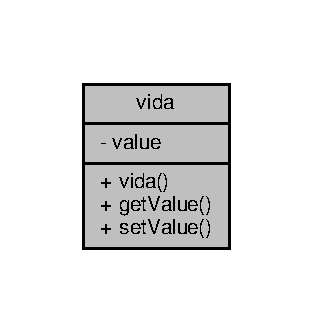
\includegraphics[width=238pt]{classvida__coll__graph}
\end{center}
\end{figure}
\subsection*{Public Member Functions}
\begin{DoxyCompactItemize}
\item 
\hyperlink{classvida_ad384ba4be61ab721939ebd0a7ed818b8}{vida} (int value\+\_\+)
\item 
\hyperlink{classvida_abfe8a67f7f8dcae0ab10ec1c0db79fd5}{vida} ()
\item 
\hyperlink{classvida_a63b5fc83a742ff15aab32c8b898b23d3}{N\+L\+O\+H\+M\+A\+N\+N\+\_\+\+D\+E\+F\+I\+N\+E\+\_\+\+T\+Y\+P\+E\+\_\+\+I\+N\+T\+R\+U\+S\+I\+VE} (\hyperlink{classvida}{vida}, \hyperlink{classvida_ae9dec2f5055b4b7b7a67be0d3c344ba4}{value})
\item 
int \hyperlink{classvida_aff59d5fa0f254f27c938bf26d5ea69d1}{get\+Value} ()
\item 
void \hyperlink{classvida_a0aa2965112fb4a5cd4497a2fc4d01544}{set\+Value} (int value\+\_\+)
\item 
float \hyperlink{classvida_a7738e842c3b8d5f8efb9df3e924895d5}{get\+Wmult} ()
\item 
float \hyperlink{classvida_a790437d520f6b3b56cf3df3886e20e8e}{get\+Hmult} ()
\item 
int \hyperlink{classvida_a29ef7f71e790ec24dea4b62fda491567}{getX} ()
\item 
int \hyperlink{classvida_a79e81325d40ab1dff09631a95b800ffa}{getY} ()
\end{DoxyCompactItemize}
\subsection*{Private Attributes}
\begin{DoxyCompactItemize}
\item 
int \hyperlink{classvida_ae9dec2f5055b4b7b7a67be0d3c344ba4}{value}
\item 
float \hyperlink{classvida_af4cfd2e27f1a6ec987e40624b7534c69}{w\+\_\+mult} =2
\item 
float \hyperlink{classvida_a5751fa7104125853e5dd42a9d9cebf6b}{h\+\_\+mult} =0.\+5
\item 
int \hyperlink{classvida_a17ff04538fab7157cac229771afaf8ef}{x} = 0.\+5
\item 
int \hyperlink{classvida_ac811d6096e5b4d9a5d4eb5aa935a242d}{y} = 0.\+7
\end{DoxyCompactItemize}


\subsection{Detailed Description}
Classe para os pontos. 

Classe utilizada para armazenar os pontos do jogador. 

\subsection{Constructor \& Destructor Documentation}
\index{vida@{vida}!vida@{vida}}
\index{vida@{vida}!vida@{vida}}
\subsubsection[{\texorpdfstring{vida(int value\+\_\+)}{vida(int value_)}}]{\setlength{\rightskip}{0pt plus 5cm}vida\+::vida (
\begin{DoxyParamCaption}
\item[{int}]{value\+\_\+}
\end{DoxyParamCaption}
)}\hypertarget{classvida_ad384ba4be61ab721939ebd0a7ed818b8}{}\label{classvida_ad384ba4be61ab721939ebd0a7ed818b8}
\index{vida@{vida}!vida@{vida}}
\index{vida@{vida}!vida@{vida}}
\subsubsection[{\texorpdfstring{vida()}{vida()}}]{\setlength{\rightskip}{0pt plus 5cm}vida\+::vida (
\begin{DoxyParamCaption}
{}
\end{DoxyParamCaption}
)}\hypertarget{classvida_abfe8a67f7f8dcae0ab10ec1c0db79fd5}{}\label{classvida_abfe8a67f7f8dcae0ab10ec1c0db79fd5}


\subsection{Member Function Documentation}
\index{vida@{vida}!get\+Hmult@{get\+Hmult}}
\index{get\+Hmult@{get\+Hmult}!vida@{vida}}
\subsubsection[{\texorpdfstring{get\+Hmult()}{getHmult()}}]{\setlength{\rightskip}{0pt plus 5cm}float vida\+::get\+Hmult (
\begin{DoxyParamCaption}
{}
\end{DoxyParamCaption}
)}\hypertarget{classvida_a790437d520f6b3b56cf3df3886e20e8e}{}\label{classvida_a790437d520f6b3b56cf3df3886e20e8e}
\index{vida@{vida}!get\+Value@{get\+Value}}
\index{get\+Value@{get\+Value}!vida@{vida}}
\subsubsection[{\texorpdfstring{get\+Value()}{getValue()}}]{\setlength{\rightskip}{0pt plus 5cm}int vida\+::get\+Value (
\begin{DoxyParamCaption}
{}
\end{DoxyParamCaption}
)}\hypertarget{classvida_aff59d5fa0f254f27c938bf26d5ea69d1}{}\label{classvida_aff59d5fa0f254f27c938bf26d5ea69d1}
\index{vida@{vida}!get\+Wmult@{get\+Wmult}}
\index{get\+Wmult@{get\+Wmult}!vida@{vida}}
\subsubsection[{\texorpdfstring{get\+Wmult()}{getWmult()}}]{\setlength{\rightskip}{0pt plus 5cm}float vida\+::get\+Wmult (
\begin{DoxyParamCaption}
{}
\end{DoxyParamCaption}
)}\hypertarget{classvida_a7738e842c3b8d5f8efb9df3e924895d5}{}\label{classvida_a7738e842c3b8d5f8efb9df3e924895d5}
\index{vida@{vida}!getX@{getX}}
\index{getX@{getX}!vida@{vida}}
\subsubsection[{\texorpdfstring{get\+X()}{getX()}}]{\setlength{\rightskip}{0pt plus 5cm}int vida\+::getX (
\begin{DoxyParamCaption}
{}
\end{DoxyParamCaption}
)}\hypertarget{classvida_a29ef7f71e790ec24dea4b62fda491567}{}\label{classvida_a29ef7f71e790ec24dea4b62fda491567}
\index{vida@{vida}!getY@{getY}}
\index{getY@{getY}!vida@{vida}}
\subsubsection[{\texorpdfstring{get\+Y()}{getY()}}]{\setlength{\rightskip}{0pt plus 5cm}int vida\+::getY (
\begin{DoxyParamCaption}
{}
\end{DoxyParamCaption}
)}\hypertarget{classvida_a79e81325d40ab1dff09631a95b800ffa}{}\label{classvida_a79e81325d40ab1dff09631a95b800ffa}
\index{vida@{vida}!N\+L\+O\+H\+M\+A\+N\+N\+\_\+\+D\+E\+F\+I\+N\+E\+\_\+\+T\+Y\+P\+E\+\_\+\+I\+N\+T\+R\+U\+S\+I\+VE@{N\+L\+O\+H\+M\+A\+N\+N\+\_\+\+D\+E\+F\+I\+N\+E\+\_\+\+T\+Y\+P\+E\+\_\+\+I\+N\+T\+R\+U\+S\+I\+VE}}
\index{N\+L\+O\+H\+M\+A\+N\+N\+\_\+\+D\+E\+F\+I\+N\+E\+\_\+\+T\+Y\+P\+E\+\_\+\+I\+N\+T\+R\+U\+S\+I\+VE@{N\+L\+O\+H\+M\+A\+N\+N\+\_\+\+D\+E\+F\+I\+N\+E\+\_\+\+T\+Y\+P\+E\+\_\+\+I\+N\+T\+R\+U\+S\+I\+VE}!vida@{vida}}
\subsubsection[{\texorpdfstring{N\+L\+O\+H\+M\+A\+N\+N\+\_\+\+D\+E\+F\+I\+N\+E\+\_\+\+T\+Y\+P\+E\+\_\+\+I\+N\+T\+R\+U\+S\+I\+V\+E(vida, value)}{NLOHMANN_DEFINE_TYPE_INTRUSIVE(vida, value)}}]{\setlength{\rightskip}{0pt plus 5cm}vida\+::\+N\+L\+O\+H\+M\+A\+N\+N\+\_\+\+D\+E\+F\+I\+N\+E\+\_\+\+T\+Y\+P\+E\+\_\+\+I\+N\+T\+R\+U\+S\+I\+VE (
\begin{DoxyParamCaption}
\item[{{\bf vida}}]{, }
\item[{{\bf value}}]{}
\end{DoxyParamCaption}
)}\hypertarget{classvida_a63b5fc83a742ff15aab32c8b898b23d3}{}\label{classvida_a63b5fc83a742ff15aab32c8b898b23d3}
\index{vida@{vida}!set\+Value@{set\+Value}}
\index{set\+Value@{set\+Value}!vida@{vida}}
\subsubsection[{\texorpdfstring{set\+Value(int value\+\_\+)}{setValue(int value_)}}]{\setlength{\rightskip}{0pt plus 5cm}void vida\+::set\+Value (
\begin{DoxyParamCaption}
\item[{int}]{value\+\_\+}
\end{DoxyParamCaption}
)}\hypertarget{classvida_a0aa2965112fb4a5cd4497a2fc4d01544}{}\label{classvida_a0aa2965112fb4a5cd4497a2fc4d01544}


\subsection{Member Data Documentation}
\index{vida@{vida}!h\+\_\+mult@{h\+\_\+mult}}
\index{h\+\_\+mult@{h\+\_\+mult}!vida@{vida}}
\subsubsection[{\texorpdfstring{h\+\_\+mult}{h_mult}}]{\setlength{\rightskip}{0pt plus 5cm}float vida\+::h\+\_\+mult =0.\+5\hspace{0.3cm}{\ttfamily [private]}}\hypertarget{classvida_a5751fa7104125853e5dd42a9d9cebf6b}{}\label{classvida_a5751fa7104125853e5dd42a9d9cebf6b}
Multiplicadores para parametrizar altura e largura \index{vida@{vida}!value@{value}}
\index{value@{value}!vida@{vida}}
\subsubsection[{\texorpdfstring{value}{value}}]{\setlength{\rightskip}{0pt plus 5cm}int vida\+::value\hspace{0.3cm}{\ttfamily [private]}}\hypertarget{classvida_ae9dec2f5055b4b7b7a67be0d3c344ba4}{}\label{classvida_ae9dec2f5055b4b7b7a67be0d3c344ba4}
quantidade de vidas \index{vida@{vida}!w\+\_\+mult@{w\+\_\+mult}}
\index{w\+\_\+mult@{w\+\_\+mult}!vida@{vida}}
\subsubsection[{\texorpdfstring{w\+\_\+mult}{w_mult}}]{\setlength{\rightskip}{0pt plus 5cm}float vida\+::w\+\_\+mult =2\hspace{0.3cm}{\ttfamily [private]}}\hypertarget{classvida_af4cfd2e27f1a6ec987e40624b7534c69}{}\label{classvida_af4cfd2e27f1a6ec987e40624b7534c69}
\index{vida@{vida}!x@{x}}
\index{x@{x}!vida@{vida}}
\subsubsection[{\texorpdfstring{x}{x}}]{\setlength{\rightskip}{0pt plus 5cm}int vida\+::x = 0.\+5\hspace{0.3cm}{\ttfamily [private]}}\hypertarget{classvida_a17ff04538fab7157cac229771afaf8ef}{}\label{classvida_a17ff04538fab7157cac229771afaf8ef}
\index{vida@{vida}!y@{y}}
\index{y@{y}!vida@{vida}}
\subsubsection[{\texorpdfstring{y}{y}}]{\setlength{\rightskip}{0pt plus 5cm}int vida\+::y = 0.\+7\hspace{0.3cm}{\ttfamily [private]}}\hypertarget{classvida_ac811d6096e5b4d9a5d4eb5aa935a242d}{}\label{classvida_ac811d6096e5b4d9a5d4eb5aa935a242d}
Posicao da vida 

The documentation for this class was generated from the following files\+:\begin{DoxyCompactItemize}
\item 
include/\hyperlink{vida_8h}{vida.\+h}\item 
src/model/\hyperlink{vida_8cpp}{vida.\+cpp}\end{DoxyCompactItemize}

\hypertarget{classview}{}\section{view Class Reference}
\label{classview}\index{view@{view}}


Classe para o view.  




{\ttfamily \#include $<$view.\+h$>$}



Collaboration diagram for view\+:
\nopagebreak
\begin{figure}[H]
\begin{center}
\leavevmode
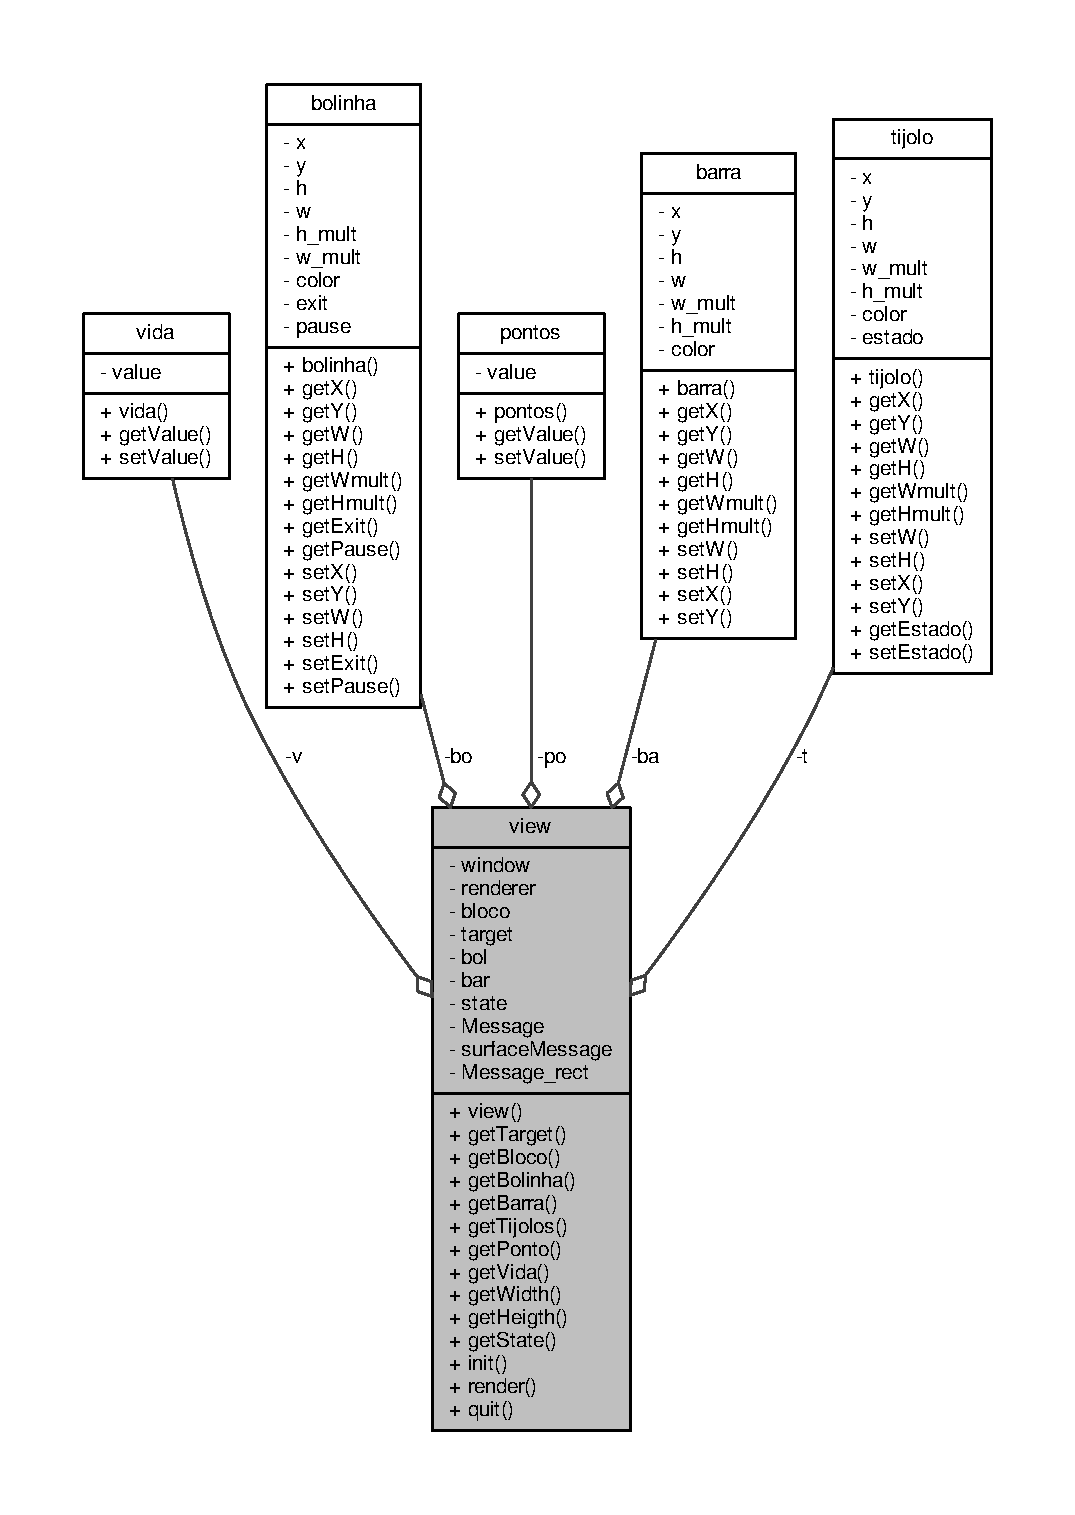
\includegraphics[width=350pt]{classview__coll__graph}
\end{center}
\end{figure}
\subsection*{Public Member Functions}
\begin{DoxyCompactItemize}
\item 
\hyperlink{classview_a809bdce6090439ac99ab0e5856c130e2}{view} (std\+::vector$<$ std\+::vector$<$ \hyperlink{classtijolo}{tijolo} $>$ $>$ \&t\+\_\+, std\+::vector$<$ \hyperlink{classbarra}{barra} $>$ \&ba\+\_\+, \hyperlink{classbolinha}{bolinha} $\ast$bo\+\_\+, \hyperlink{classpontos}{pontos} $\ast$po\+\_\+, \hyperlink{classvida}{vida} $\ast$v\+\_\+)
\begin{DoxyCompactList}\small\item\em Construtor do view. \end{DoxyCompactList}\item 
void \hyperlink{classview_afa73cff596b36c7009ee17383d039750}{render\+\_\+text} (S\+D\+L\+\_\+\+Renderer $\ast$\hyperlink{classview_a8d7b3ec0a0641d24cdc3b04949f5df45}{renderer}, int x, int y, const char $\ast$text, T\+T\+F\+\_\+\+Font $\ast$font, S\+D\+L\+\_\+\+Rect $\ast$rect, S\+D\+L\+\_\+\+Color $\ast$color)
\begin{DoxyCompactList}\small\item\em Renderiza um texto. \end{DoxyCompactList}\item 
int \hyperlink{classview_a21d953772b41dd9c08c9ea9895e002d7}{init} ()
\begin{DoxyCompactList}\small\item\em Rotina de inicializacao. \end{DoxyCompactList}\item 
int \hyperlink{classview_ac0e552fdef69accb371177ef955e1b38}{init\+Client} ()
\item 
void \hyperlink{classview_a6ce9703fff0ea8ae911fee1d24a418e0}{render} (int user)
\begin{DoxyCompactList}\small\item\em Renderizacao. \end{DoxyCompactList}\item 
void \hyperlink{classview_ad8c046a243e52ee4f902abec6fbec9bb}{quit} ()
\begin{DoxyCompactList}\small\item\em Encerramento. \end{DoxyCompactList}\item 
void \hyperlink{classview_a23918beecf637e8226bc1ff64a67e811}{perdeu} (int user)
\begin{DoxyCompactList}\small\item\em Derrota. \end{DoxyCompactList}\item 
void \hyperlink{classview_af4509b82ea85ae1e29b0fa51e2156f73}{ganhou} (int user)
\begin{DoxyCompactList}\small\item\em Vitoria Singleplayer. \end{DoxyCompactList}\item 
void \hyperlink{classview_a81553c85d81a253c49b002440a039fd3}{ganhou\+Multi} (int user\+\_\+id)
\begin{DoxyCompactList}\small\item\em Vitoria Multiplayer. \end{DoxyCompactList}\item 
int \hyperlink{classview_a987e7c197e87c90671d6f5347d2dab9d}{window\+\_\+create} (int size)
\item 
int \hyperlink{classview_a257d50065961954053fbf5402b2e2968}{quantidade\+Tijolos} ()
\item 
S\+D\+L\+\_\+\+Rect $\ast$ \hyperlink{classview_a4bf37f4171f4bb15c0e5b4ab8c2a9faa}{get\+Target} ()
\item 
S\+D\+L\+\_\+\+Rect $\ast$ \hyperlink{classview_a8b12f1f06de39d6e9f70f54a9281e05c}{get\+Bloco} ()
\item 
S\+D\+L\+\_\+\+Rect $\ast$ \hyperlink{classview_a8eb9d89d9b55a5d2ee529c96e0dc246a}{get\+Bolinha} ()
\item 
S\+D\+L\+\_\+\+Rect $\ast$ \hyperlink{classview_a57b60e5da21e0484081d71c69ba4d03e}{get\+Barra} ()
\item 
std\+::vector$<$ \hyperlink{classbarra}{barra} $>$ \& \hyperlink{classview_abae031de8054f66f9b0e7a5caabdc513}{get\+Barras} ()
\item 
std\+::vector$<$ std\+::vector$<$ \hyperlink{classtijolo}{tijolo} $>$ $>$ \& \hyperlink{classview_aba52b9c597c0b8acfacf96f21547977a}{get\+Tijolos} ()
\item 
\hyperlink{classpontos}{pontos} $\ast$ \hyperlink{classview_a6cd53aa4df2642579992803a18f0bc8b}{get\+Ponto} ()
\item 
\hyperlink{classvida}{vida} $\ast$ \hyperlink{classview_aa33f3e6bf59ada95ee9fd0bff5af22c0}{get\+Vida} ()
\item 
int \hyperlink{classview_aba1c490d357bb58f4aa9218cb96b42b0}{get\+Width} ()
\item 
int \hyperlink{classview_af2cf0c4a4d7cd84f0155ae1ad6a51d0a}{get\+Heigth} ()
\item 
const Uint8 $\ast$ \hyperlink{classview_a5dd0f6c8f5d5f9123353986607c7fb77}{get\+State} ()
\end{DoxyCompactItemize}
\subsection*{Private Attributes}
\begin{DoxyCompactItemize}
\item 
std\+::vector$<$ std\+::vector$<$ \hyperlink{classtijolo}{tijolo} $>$ $>$ \& \hyperlink{classview_adf9164a1a6940c4224d67b5c33424f10}{t}
\item 
\hyperlink{classbolinha}{bolinha} $\ast$ \hyperlink{classview_a9d44d190dd69b906bfeaac4559ee454e}{bo}
\item 
std\+::vector$<$ \hyperlink{classbarra}{barra} $>$ \& \hyperlink{classview_a38f555c4b8b985a9788a4196f5be917f}{ba}
\item 
\hyperlink{classpontos}{pontos} $\ast$ \hyperlink{classview_a8dc345a9799a79220ecca66c4cd3e8ff}{po}
\item 
\hyperlink{classvida}{vida} $\ast$ \hyperlink{classview_ae0f8e281f5f7937d84f435437ce03546}{v}
\item 
S\+D\+L\+\_\+\+Window $\ast$ \hyperlink{classview_ade09c2dbabd1bf59ffaf625156c514f0}{window}
\item 
S\+D\+L\+\_\+\+Renderer $\ast$ \hyperlink{classview_a8d7b3ec0a0641d24cdc3b04949f5df45}{renderer}
\item 
S\+D\+L\+\_\+\+Rect \hyperlink{classview_ae22fb0558e890ff6ace089b603e2d6d8}{bloco}
\item 
S\+D\+L\+\_\+\+Rect \hyperlink{classview_a49a628eedba666db008f8c07b96e3a51}{target}
\item 
S\+D\+L\+\_\+\+Rect \hyperlink{classview_a72e360ef18105e2c565f17be3768027d}{bol}
\item 
S\+D\+L\+\_\+\+Rect \hyperlink{classview_a9c94bf9b55b5c24c5a9289d82a969ebb}{bar}
\item 
const Uint8 $\ast$ \hyperlink{classview_a6fd7fc350d9ad94dfd47e324b107e8ce}{state}
\item 
T\+T\+F\+\_\+\+Font $\ast$ \hyperlink{classview_ad17acebf948f7f42aa7cb8f88a38fe21}{Font}
\item 
S\+D\+L\+\_\+\+Rect \hyperlink{classview_af1b48d8a8f7f9e16800f9d842717ed2c}{Message\+\_\+\+Vida\+\_\+rect}
\item 
S\+D\+L\+\_\+\+Rect \hyperlink{classview_aba853e73ed61ec0078ff6e56bb57e702}{Message\+\_\+\+Fim\+\_\+rect}
\item 
S\+D\+L\+\_\+\+Rect \hyperlink{classview_ada3fc542a5e8b9d9e002665b37af781b}{Message\+\_\+\+Pontos\+\_\+rect}
\item 
S\+D\+L\+\_\+\+Rect \hyperlink{classview_a1a7059536cb8e091ff7d4a4f2526bcce}{Message\+\_\+\+Vida\+Value\+\_\+rect}
\item 
S\+D\+L\+\_\+\+Rect \hyperlink{classview_ade4cd2992600a54f7cb1f9f20876cd75}{Message\+\_\+\+Point\+Value\+\_\+rect}
\end{DoxyCompactItemize}


\subsection{Detailed Description}
Classe para o view. 

Esta é a classe para o view. Ela recebe todos os objetos que precisam ser mostrados em tela, e utiliza a biblioteca S\+D\+L2 para isso. 

\subsection{Constructor \& Destructor Documentation}
\index{view@{view}!view@{view}}
\index{view@{view}!view@{view}}
\subsubsection[{\texorpdfstring{view(std\+::vector$<$ std\+::vector$<$ tijolo $>$ $>$ \&t\+\_\+, std\+::vector$<$ barra $>$ \&ba\+\_\+, bolinha $\ast$bo\+\_\+, pontos $\ast$po\+\_\+, vida $\ast$v\+\_\+)}{view(std::vector< std::vector< tijolo > > &t_, std::vector< barra > &ba_, bolinha *bo_, pontos *po_, vida *v_)}}]{\setlength{\rightskip}{0pt plus 5cm}view\+::view (
\begin{DoxyParamCaption}
\item[{std\+::vector$<$ std\+::vector$<$ {\bf tijolo} $>$ $>$ \&}]{t\+\_\+, }
\item[{std\+::vector$<$ {\bf barra} $>$ \&}]{ba\+\_\+, }
\item[{{\bf bolinha} $\ast$}]{bo\+\_\+, }
\item[{{\bf pontos} $\ast$}]{po\+\_\+, }
\item[{{\bf vida} $\ast$}]{v\+\_\+}
\end{DoxyParamCaption}
)}\hypertarget{classview_a809bdce6090439ac99ab0e5856c130e2}{}\label{classview_a809bdce6090439ac99ab0e5856c130e2}


Construtor do view. 

Recebe um tudo o que for ser mostrado em tela


\begin{DoxyParams}{Parameters}
{\em t\+\_\+} & objeto tijolo \\
\hline
{\em ba\+\_\+} & objeto barra \\
\hline
{\em bo\+\_\+} & objeto bolinha \\
\hline
{\em po\+\_\+} & objeto pontos \\
\hline
{\em v\+\_\+} & objeto vida \\
\hline
\end{DoxyParams}


\subsection{Member Function Documentation}
\index{view@{view}!ganhou@{ganhou}}
\index{ganhou@{ganhou}!view@{view}}
\subsubsection[{\texorpdfstring{ganhou(int user)}{ganhou(int user)}}]{\setlength{\rightskip}{0pt plus 5cm}void view\+::ganhou (
\begin{DoxyParamCaption}
\item[{int}]{user}
\end{DoxyParamCaption}
)}\hypertarget{classview_af4509b82ea85ae1e29b0fa51e2156f73}{}\label{classview_af4509b82ea85ae1e29b0fa51e2156f73}


Vitoria Singleplayer. 

Sequencia de acoes para quando um jogador ganha \index{view@{view}!ganhou\+Multi@{ganhou\+Multi}}
\index{ganhou\+Multi@{ganhou\+Multi}!view@{view}}
\subsubsection[{\texorpdfstring{ganhou\+Multi(int user\+\_\+id)}{ganhouMulti(int user_id)}}]{\setlength{\rightskip}{0pt plus 5cm}void view\+::ganhou\+Multi (
\begin{DoxyParamCaption}
\item[{int}]{user\+\_\+id}
\end{DoxyParamCaption}
)}\hypertarget{classview_a81553c85d81a253c49b002440a039fd3}{}\label{classview_a81553c85d81a253c49b002440a039fd3}


Vitoria Multiplayer. 

Sequencia de acoes para quando um jogador ganha no multiplayer \index{view@{view}!get\+Barra@{get\+Barra}}
\index{get\+Barra@{get\+Barra}!view@{view}}
\subsubsection[{\texorpdfstring{get\+Barra()}{getBarra()}}]{\setlength{\rightskip}{0pt plus 5cm}S\+D\+L\+\_\+\+Rect $\ast$ view\+::get\+Barra (
\begin{DoxyParamCaption}
{}
\end{DoxyParamCaption}
)}\hypertarget{classview_a57b60e5da21e0484081d71c69ba4d03e}{}\label{classview_a57b60e5da21e0484081d71c69ba4d03e}
\index{view@{view}!get\+Barras@{get\+Barras}}
\index{get\+Barras@{get\+Barras}!view@{view}}
\subsubsection[{\texorpdfstring{get\+Barras()}{getBarras()}}]{\setlength{\rightskip}{0pt plus 5cm}std\+::vector$<$ {\bf barra} $>$ \& view\+::get\+Barras (
\begin{DoxyParamCaption}
{}
\end{DoxyParamCaption}
)}\hypertarget{classview_abae031de8054f66f9b0e7a5caabdc513}{}\label{classview_abae031de8054f66f9b0e7a5caabdc513}
\index{view@{view}!get\+Bloco@{get\+Bloco}}
\index{get\+Bloco@{get\+Bloco}!view@{view}}
\subsubsection[{\texorpdfstring{get\+Bloco()}{getBloco()}}]{\setlength{\rightskip}{0pt plus 5cm}S\+D\+L\+\_\+\+Rect $\ast$ view\+::get\+Bloco (
\begin{DoxyParamCaption}
{}
\end{DoxyParamCaption}
)}\hypertarget{classview_a8b12f1f06de39d6e9f70f54a9281e05c}{}\label{classview_a8b12f1f06de39d6e9f70f54a9281e05c}
\index{view@{view}!get\+Bolinha@{get\+Bolinha}}
\index{get\+Bolinha@{get\+Bolinha}!view@{view}}
\subsubsection[{\texorpdfstring{get\+Bolinha()}{getBolinha()}}]{\setlength{\rightskip}{0pt plus 5cm}S\+D\+L\+\_\+\+Rect $\ast$ view\+::get\+Bolinha (
\begin{DoxyParamCaption}
{}
\end{DoxyParamCaption}
)}\hypertarget{classview_a8eb9d89d9b55a5d2ee529c96e0dc246a}{}\label{classview_a8eb9d89d9b55a5d2ee529c96e0dc246a}
\index{view@{view}!get\+Heigth@{get\+Heigth}}
\index{get\+Heigth@{get\+Heigth}!view@{view}}
\subsubsection[{\texorpdfstring{get\+Heigth()}{getHeigth()}}]{\setlength{\rightskip}{0pt plus 5cm}int view\+::get\+Heigth (
\begin{DoxyParamCaption}
{}
\end{DoxyParamCaption}
)}\hypertarget{classview_af2cf0c4a4d7cd84f0155ae1ad6a51d0a}{}\label{classview_af2cf0c4a4d7cd84f0155ae1ad6a51d0a}
\index{view@{view}!get\+Ponto@{get\+Ponto}}
\index{get\+Ponto@{get\+Ponto}!view@{view}}
\subsubsection[{\texorpdfstring{get\+Ponto()}{getPonto()}}]{\setlength{\rightskip}{0pt plus 5cm}{\bf pontos} $\ast$ view\+::get\+Ponto (
\begin{DoxyParamCaption}
{}
\end{DoxyParamCaption}
)}\hypertarget{classview_a6cd53aa4df2642579992803a18f0bc8b}{}\label{classview_a6cd53aa4df2642579992803a18f0bc8b}
\index{view@{view}!get\+State@{get\+State}}
\index{get\+State@{get\+State}!view@{view}}
\subsubsection[{\texorpdfstring{get\+State()}{getState()}}]{\setlength{\rightskip}{0pt plus 5cm}const Uint8 $\ast$ view\+::get\+State (
\begin{DoxyParamCaption}
{}
\end{DoxyParamCaption}
)}\hypertarget{classview_a5dd0f6c8f5d5f9123353986607c7fb77}{}\label{classview_a5dd0f6c8f5d5f9123353986607c7fb77}
\index{view@{view}!get\+Target@{get\+Target}}
\index{get\+Target@{get\+Target}!view@{view}}
\subsubsection[{\texorpdfstring{get\+Target()}{getTarget()}}]{\setlength{\rightskip}{0pt plus 5cm}S\+D\+L\+\_\+\+Rect $\ast$ view\+::get\+Target (
\begin{DoxyParamCaption}
{}
\end{DoxyParamCaption}
)}\hypertarget{classview_a4bf37f4171f4bb15c0e5b4ab8c2a9faa}{}\label{classview_a4bf37f4171f4bb15c0e5b4ab8c2a9faa}
\index{view@{view}!get\+Tijolos@{get\+Tijolos}}
\index{get\+Tijolos@{get\+Tijolos}!view@{view}}
\subsubsection[{\texorpdfstring{get\+Tijolos()}{getTijolos()}}]{\setlength{\rightskip}{0pt plus 5cm}std\+::vector$<$ std\+::vector$<$ {\bf tijolo} $>$ $>$ \& view\+::get\+Tijolos (
\begin{DoxyParamCaption}
{}
\end{DoxyParamCaption}
)}\hypertarget{classview_aba52b9c597c0b8acfacf96f21547977a}{}\label{classview_aba52b9c597c0b8acfacf96f21547977a}
\index{view@{view}!get\+Vida@{get\+Vida}}
\index{get\+Vida@{get\+Vida}!view@{view}}
\subsubsection[{\texorpdfstring{get\+Vida()}{getVida()}}]{\setlength{\rightskip}{0pt plus 5cm}{\bf vida} $\ast$ view\+::get\+Vida (
\begin{DoxyParamCaption}
{}
\end{DoxyParamCaption}
)}\hypertarget{classview_aa33f3e6bf59ada95ee9fd0bff5af22c0}{}\label{classview_aa33f3e6bf59ada95ee9fd0bff5af22c0}
\index{view@{view}!get\+Width@{get\+Width}}
\index{get\+Width@{get\+Width}!view@{view}}
\subsubsection[{\texorpdfstring{get\+Width()}{getWidth()}}]{\setlength{\rightskip}{0pt plus 5cm}int view\+::get\+Width (
\begin{DoxyParamCaption}
{}
\end{DoxyParamCaption}
)}\hypertarget{classview_aba1c490d357bb58f4aa9218cb96b42b0}{}\label{classview_aba1c490d357bb58f4aa9218cb96b42b0}
\index{view@{view}!init@{init}}
\index{init@{init}!view@{view}}
\subsubsection[{\texorpdfstring{init()}{init()}}]{\setlength{\rightskip}{0pt plus 5cm}int view\+::init (
\begin{DoxyParamCaption}
{}
\end{DoxyParamCaption}
)}\hypertarget{classview_a21d953772b41dd9c08c9ea9895e002d7}{}\label{classview_a21d953772b41dd9c08c9ea9895e002d7}


Rotina de inicializacao. 

Sequencia de acoes que inicializam a janela de visualizacao \index{view@{view}!init\+Client@{init\+Client}}
\index{init\+Client@{init\+Client}!view@{view}}
\subsubsection[{\texorpdfstring{init\+Client()}{initClient()}}]{\setlength{\rightskip}{0pt plus 5cm}int view\+::init\+Client (
\begin{DoxyParamCaption}
{}
\end{DoxyParamCaption}
)}\hypertarget{classview_ac0e552fdef69accb371177ef955e1b38}{}\label{classview_ac0e552fdef69accb371177ef955e1b38}
\index{view@{view}!perdeu@{perdeu}}
\index{perdeu@{perdeu}!view@{view}}
\subsubsection[{\texorpdfstring{perdeu(int user)}{perdeu(int user)}}]{\setlength{\rightskip}{0pt plus 5cm}void view\+::perdeu (
\begin{DoxyParamCaption}
\item[{int}]{user}
\end{DoxyParamCaption}
)}\hypertarget{classview_a23918beecf637e8226bc1ff64a67e811}{}\label{classview_a23918beecf637e8226bc1ff64a67e811}


Derrota. 

Sequencia de acoes para quando um jogador perde \index{view@{view}!quantidade\+Tijolos@{quantidade\+Tijolos}}
\index{quantidade\+Tijolos@{quantidade\+Tijolos}!view@{view}}
\subsubsection[{\texorpdfstring{quantidade\+Tijolos()}{quantidadeTijolos()}}]{\setlength{\rightskip}{0pt plus 5cm}int view\+::quantidade\+Tijolos (
\begin{DoxyParamCaption}
{}
\end{DoxyParamCaption}
)}\hypertarget{classview_a257d50065961954053fbf5402b2e2968}{}\label{classview_a257d50065961954053fbf5402b2e2968}
\index{view@{view}!quit@{quit}}
\index{quit@{quit}!view@{view}}
\subsubsection[{\texorpdfstring{quit()}{quit()}}]{\setlength{\rightskip}{0pt plus 5cm}void view\+::quit (
\begin{DoxyParamCaption}
{}
\end{DoxyParamCaption}
)}\hypertarget{classview_ad8c046a243e52ee4f902abec6fbec9bb}{}\label{classview_ad8c046a243e52ee4f902abec6fbec9bb}


Encerramento. 

Metodo que encerra os objetos de visualizacao e fecha o programa \index{view@{view}!render@{render}}
\index{render@{render}!view@{view}}
\subsubsection[{\texorpdfstring{render(int user)}{render(int user)}}]{\setlength{\rightskip}{0pt plus 5cm}void view\+::render (
\begin{DoxyParamCaption}
\item[{int}]{user}
\end{DoxyParamCaption}
)}\hypertarget{classview_a6ce9703fff0ea8ae911fee1d24a418e0}{}\label{classview_a6ce9703fff0ea8ae911fee1d24a418e0}


Renderizacao. 

Metodo que renderiza todos os objetos a cada ciclo definido \index{view@{view}!render\+\_\+text@{render\+\_\+text}}
\index{render\+\_\+text@{render\+\_\+text}!view@{view}}
\subsubsection[{\texorpdfstring{render\+\_\+text(\+S\+D\+L\+\_\+\+Renderer $\ast$renderer, int x, int y, const char $\ast$text, T\+T\+F\+\_\+\+Font $\ast$font, S\+D\+L\+\_\+\+Rect $\ast$rect, S\+D\+L\+\_\+\+Color $\ast$color)}{render_text(SDL_Renderer *renderer, int x, int y, const char *text, TTF_Font *font, SDL_Rect *rect, SDL_Color *color)}}]{\setlength{\rightskip}{0pt plus 5cm}void view\+::render\+\_\+text (
\begin{DoxyParamCaption}
\item[{S\+D\+L\+\_\+\+Renderer $\ast$}]{renderer, }
\item[{int}]{x, }
\item[{int}]{y, }
\item[{const char $\ast$}]{text, }
\item[{T\+T\+F\+\_\+\+Font $\ast$}]{font, }
\item[{S\+D\+L\+\_\+\+Rect $\ast$}]{rect, }
\item[{S\+D\+L\+\_\+\+Color $\ast$}]{color}
\end{DoxyParamCaption}
)}\hypertarget{classview_afa73cff596b36c7009ee17383d039750}{}\label{classview_afa73cff596b36c7009ee17383d039750}


Renderiza um texto. 

Renderiza um texto em uma dada posicao, fonte e cor. Todos esses parametros sao passados na funcao


\begin{DoxyParams}{Parameters}
{\em renderer} & objeto S\+D\+L\+\_\+\+Renderer alocado previamente \\
\hline
{\em x} & posicao x do texto \\
\hline
{\em y} & posicao y do texto \\
\hline
{\em text} & vetor de chars que sera renderizado \\
\hline
{\em font} & objeto T\+T\+F\+\_\+\+Font com a fonte do texto a ser renderizado \\
\hline
{\em rect} & objeto S\+D\+L\+\_\+\+Rect alocado previamente \\
\hline
{\em color} & objeto S\+D\+L\+\_\+\+Color com a cor do texto a ser renderizado \\
\hline
\end{DoxyParams}
\index{view@{view}!window\+\_\+create@{window\+\_\+create}}
\index{window\+\_\+create@{window\+\_\+create}!view@{view}}
\subsubsection[{\texorpdfstring{window\+\_\+create(int size)}{window_create(int size)}}]{\setlength{\rightskip}{0pt plus 5cm}int view\+::window\+\_\+create (
\begin{DoxyParamCaption}
\item[{int}]{size}
\end{DoxyParamCaption}
)}\hypertarget{classview_a987e7c197e87c90671d6f5347d2dab9d}{}\label{classview_a987e7c197e87c90671d6f5347d2dab9d}


\subsection{Member Data Documentation}
\index{view@{view}!ba@{ba}}
\index{ba@{ba}!view@{view}}
\subsubsection[{\texorpdfstring{ba}{ba}}]{\setlength{\rightskip}{0pt plus 5cm}std\+::vector$<${\bf barra}$>$\& view\+::ba\hspace{0.3cm}{\ttfamily [private]}}\hypertarget{classview_a38f555c4b8b985a9788a4196f5be917f}{}\label{classview_a38f555c4b8b985a9788a4196f5be917f}
barra (alocado previamente) \index{view@{view}!bar@{bar}}
\index{bar@{bar}!view@{view}}
\subsubsection[{\texorpdfstring{bar}{bar}}]{\setlength{\rightskip}{0pt plus 5cm}S\+D\+L\+\_\+\+Rect view\+::bar\hspace{0.3cm}{\ttfamily [private]}}\hypertarget{classview_a9c94bf9b55b5c24c5a9289d82a969ebb}{}\label{classview_a9c94bf9b55b5c24c5a9289d82a969ebb}
\index{view@{view}!bloco@{bloco}}
\index{bloco@{bloco}!view@{view}}
\subsubsection[{\texorpdfstring{bloco}{bloco}}]{\setlength{\rightskip}{0pt plus 5cm}S\+D\+L\+\_\+\+Rect view\+::bloco\hspace{0.3cm}{\ttfamily [private]}}\hypertarget{classview_ae22fb0558e890ff6ace089b603e2d6d8}{}\label{classview_ae22fb0558e890ff6ace089b603e2d6d8}
\index{view@{view}!bo@{bo}}
\index{bo@{bo}!view@{view}}
\subsubsection[{\texorpdfstring{bo}{bo}}]{\setlength{\rightskip}{0pt plus 5cm}{\bf bolinha}$\ast$ view\+::bo\hspace{0.3cm}{\ttfamily [private]}}\hypertarget{classview_a9d44d190dd69b906bfeaac4559ee454e}{}\label{classview_a9d44d190dd69b906bfeaac4559ee454e}
bolinha (alocado previamente) \index{view@{view}!bol@{bol}}
\index{bol@{bol}!view@{view}}
\subsubsection[{\texorpdfstring{bol}{bol}}]{\setlength{\rightskip}{0pt plus 5cm}S\+D\+L\+\_\+\+Rect view\+::bol\hspace{0.3cm}{\ttfamily [private]}}\hypertarget{classview_a72e360ef18105e2c565f17be3768027d}{}\label{classview_a72e360ef18105e2c565f17be3768027d}
\index{view@{view}!Font@{Font}}
\index{Font@{Font}!view@{view}}
\subsubsection[{\texorpdfstring{Font}{Font}}]{\setlength{\rightskip}{0pt plus 5cm}T\+T\+F\+\_\+\+Font$\ast$ view\+::\+Font\hspace{0.3cm}{\ttfamily [private]}}\hypertarget{classview_ad17acebf948f7f42aa7cb8f88a38fe21}{}\label{classview_ad17acebf948f7f42aa7cb8f88a38fe21}
\index{view@{view}!Message\+\_\+\+Fim\+\_\+rect@{Message\+\_\+\+Fim\+\_\+rect}}
\index{Message\+\_\+\+Fim\+\_\+rect@{Message\+\_\+\+Fim\+\_\+rect}!view@{view}}
\subsubsection[{\texorpdfstring{Message\+\_\+\+Fim\+\_\+rect}{Message_Fim_rect}}]{\setlength{\rightskip}{0pt plus 5cm}S\+D\+L\+\_\+\+Rect view\+::\+Message\+\_\+\+Fim\+\_\+rect\hspace{0.3cm}{\ttfamily [private]}}\hypertarget{classview_aba853e73ed61ec0078ff6e56bb57e702}{}\label{classview_aba853e73ed61ec0078ff6e56bb57e702}
\index{view@{view}!Message\+\_\+\+Point\+Value\+\_\+rect@{Message\+\_\+\+Point\+Value\+\_\+rect}}
\index{Message\+\_\+\+Point\+Value\+\_\+rect@{Message\+\_\+\+Point\+Value\+\_\+rect}!view@{view}}
\subsubsection[{\texorpdfstring{Message\+\_\+\+Point\+Value\+\_\+rect}{Message_PointValue_rect}}]{\setlength{\rightskip}{0pt plus 5cm}S\+D\+L\+\_\+\+Rect view\+::\+Message\+\_\+\+Point\+Value\+\_\+rect\hspace{0.3cm}{\ttfamily [private]}}\hypertarget{classview_ade4cd2992600a54f7cb1f9f20876cd75}{}\label{classview_ade4cd2992600a54f7cb1f9f20876cd75}
\index{view@{view}!Message\+\_\+\+Pontos\+\_\+rect@{Message\+\_\+\+Pontos\+\_\+rect}}
\index{Message\+\_\+\+Pontos\+\_\+rect@{Message\+\_\+\+Pontos\+\_\+rect}!view@{view}}
\subsubsection[{\texorpdfstring{Message\+\_\+\+Pontos\+\_\+rect}{Message_Pontos_rect}}]{\setlength{\rightskip}{0pt plus 5cm}S\+D\+L\+\_\+\+Rect view\+::\+Message\+\_\+\+Pontos\+\_\+rect\hspace{0.3cm}{\ttfamily [private]}}\hypertarget{classview_ada3fc542a5e8b9d9e002665b37af781b}{}\label{classview_ada3fc542a5e8b9d9e002665b37af781b}
\index{view@{view}!Message\+\_\+\+Vida\+\_\+rect@{Message\+\_\+\+Vida\+\_\+rect}}
\index{Message\+\_\+\+Vida\+\_\+rect@{Message\+\_\+\+Vida\+\_\+rect}!view@{view}}
\subsubsection[{\texorpdfstring{Message\+\_\+\+Vida\+\_\+rect}{Message_Vida_rect}}]{\setlength{\rightskip}{0pt plus 5cm}S\+D\+L\+\_\+\+Rect view\+::\+Message\+\_\+\+Vida\+\_\+rect\hspace{0.3cm}{\ttfamily [private]}}\hypertarget{classview_af1b48d8a8f7f9e16800f9d842717ed2c}{}\label{classview_af1b48d8a8f7f9e16800f9d842717ed2c}
\index{view@{view}!Message\+\_\+\+Vida\+Value\+\_\+rect@{Message\+\_\+\+Vida\+Value\+\_\+rect}}
\index{Message\+\_\+\+Vida\+Value\+\_\+rect@{Message\+\_\+\+Vida\+Value\+\_\+rect}!view@{view}}
\subsubsection[{\texorpdfstring{Message\+\_\+\+Vida\+Value\+\_\+rect}{Message_VidaValue_rect}}]{\setlength{\rightskip}{0pt plus 5cm}S\+D\+L\+\_\+\+Rect view\+::\+Message\+\_\+\+Vida\+Value\+\_\+rect\hspace{0.3cm}{\ttfamily [private]}}\hypertarget{classview_a1a7059536cb8e091ff7d4a4f2526bcce}{}\label{classview_a1a7059536cb8e091ff7d4a4f2526bcce}
\index{view@{view}!po@{po}}
\index{po@{po}!view@{view}}
\subsubsection[{\texorpdfstring{po}{po}}]{\setlength{\rightskip}{0pt plus 5cm}{\bf pontos}$\ast$ view\+::po\hspace{0.3cm}{\ttfamily [private]}}\hypertarget{classview_a8dc345a9799a79220ecca66c4cd3e8ff}{}\label{classview_a8dc345a9799a79220ecca66c4cd3e8ff}
pontos (alocado previamente) \index{view@{view}!renderer@{renderer}}
\index{renderer@{renderer}!view@{view}}
\subsubsection[{\texorpdfstring{renderer}{renderer}}]{\setlength{\rightskip}{0pt plus 5cm}S\+D\+L\+\_\+\+Renderer$\ast$ view\+::renderer\hspace{0.3cm}{\ttfamily [private]}}\hypertarget{classview_a8d7b3ec0a0641d24cdc3b04949f5df45}{}\label{classview_a8d7b3ec0a0641d24cdc3b04949f5df45}
\index{view@{view}!state@{state}}
\index{state@{state}!view@{view}}
\subsubsection[{\texorpdfstring{state}{state}}]{\setlength{\rightskip}{0pt plus 5cm}const Uint8$\ast$ view\+::state\hspace{0.3cm}{\ttfamily [private]}}\hypertarget{classview_a6fd7fc350d9ad94dfd47e324b107e8ce}{}\label{classview_a6fd7fc350d9ad94dfd47e324b107e8ce}
\index{view@{view}!t@{t}}
\index{t@{t}!view@{view}}
\subsubsection[{\texorpdfstring{t}{t}}]{\setlength{\rightskip}{0pt plus 5cm}std\+::vector$<$std\+::vector$<${\bf tijolo}$>$ $>$\& view\+::t\hspace{0.3cm}{\ttfamily [private]}}\hypertarget{classview_adf9164a1a6940c4224d67b5c33424f10}{}\label{classview_adf9164a1a6940c4224d67b5c33424f10}
tijolo (alocado previamente) \index{view@{view}!target@{target}}
\index{target@{target}!view@{view}}
\subsubsection[{\texorpdfstring{target}{target}}]{\setlength{\rightskip}{0pt plus 5cm}S\+D\+L\+\_\+\+Rect view\+::target\hspace{0.3cm}{\ttfamily [private]}}\hypertarget{classview_a49a628eedba666db008f8c07b96e3a51}{}\label{classview_a49a628eedba666db008f8c07b96e3a51}
\index{view@{view}!v@{v}}
\index{v@{v}!view@{view}}
\subsubsection[{\texorpdfstring{v}{v}}]{\setlength{\rightskip}{0pt plus 5cm}{\bf vida}$\ast$ view\+::v\hspace{0.3cm}{\ttfamily [private]}}\hypertarget{classview_ae0f8e281f5f7937d84f435437ce03546}{}\label{classview_ae0f8e281f5f7937d84f435437ce03546}
vida (alocado previamente) \index{view@{view}!window@{window}}
\index{window@{window}!view@{view}}
\subsubsection[{\texorpdfstring{window}{window}}]{\setlength{\rightskip}{0pt plus 5cm}S\+D\+L\+\_\+\+Window$\ast$ view\+::window\hspace{0.3cm}{\ttfamily [private]}}\hypertarget{classview_ade09c2dbabd1bf59ffaf625156c514f0}{}\label{classview_ade09c2dbabd1bf59ffaf625156c514f0}


The documentation for this class was generated from the following files\+:\begin{DoxyCompactItemize}
\item 
include/\hyperlink{view_8h}{view.\+h}\item 
src/view/\hyperlink{view_8cpp}{view.\+cpp}\end{DoxyCompactItemize}

\chapter{File Documentation}
\hypertarget{barra_8h}{}\section{include/barra.h File Reference}
\label{barra_8h}\index{include/barra.\+h@{include/barra.\+h}}
This graph shows which files directly or indirectly include this file\+:
\nopagebreak
\begin{figure}[H]
\begin{center}
\leavevmode
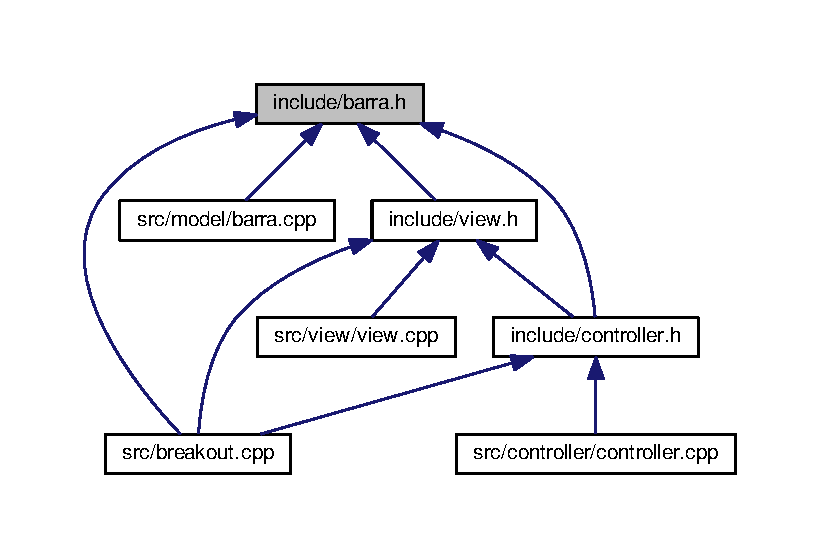
\includegraphics[width=350pt]{barra_8h__dep__incl}
\end{center}
\end{figure}
\subsection*{Classes}
\begin{DoxyCompactItemize}
\item 
class \hyperlink{classbarra}{barra}
\begin{DoxyCompactList}\small\item\em Classe para a barra. \end{DoxyCompactList}\end{DoxyCompactItemize}

\hypertarget{bolinha_8h}{}\section{include/bolinha.h File Reference}
\label{bolinha_8h}\index{include/bolinha.\+h@{include/bolinha.\+h}}
{\ttfamily \#include \char`\"{}json.\+hpp\char`\"{}}\\*
Include dependency graph for bolinha.\+h\+:
\nopagebreak
\begin{figure}[H]
\begin{center}
\leavevmode
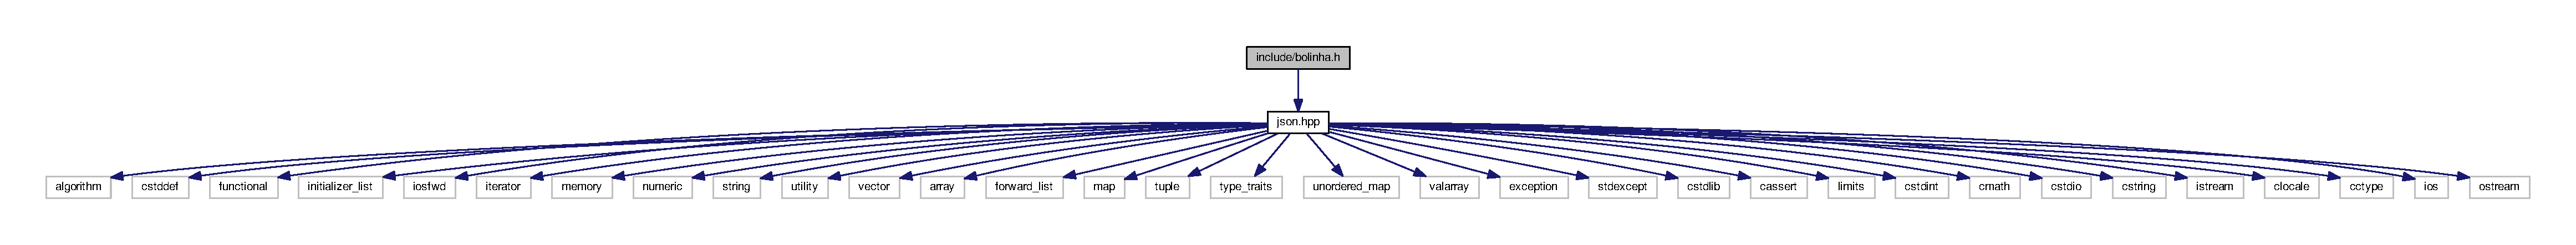
\includegraphics[width=350pt]{bolinha_8h__incl}
\end{center}
\end{figure}
This graph shows which files directly or indirectly include this file\+:
\nopagebreak
\begin{figure}[H]
\begin{center}
\leavevmode
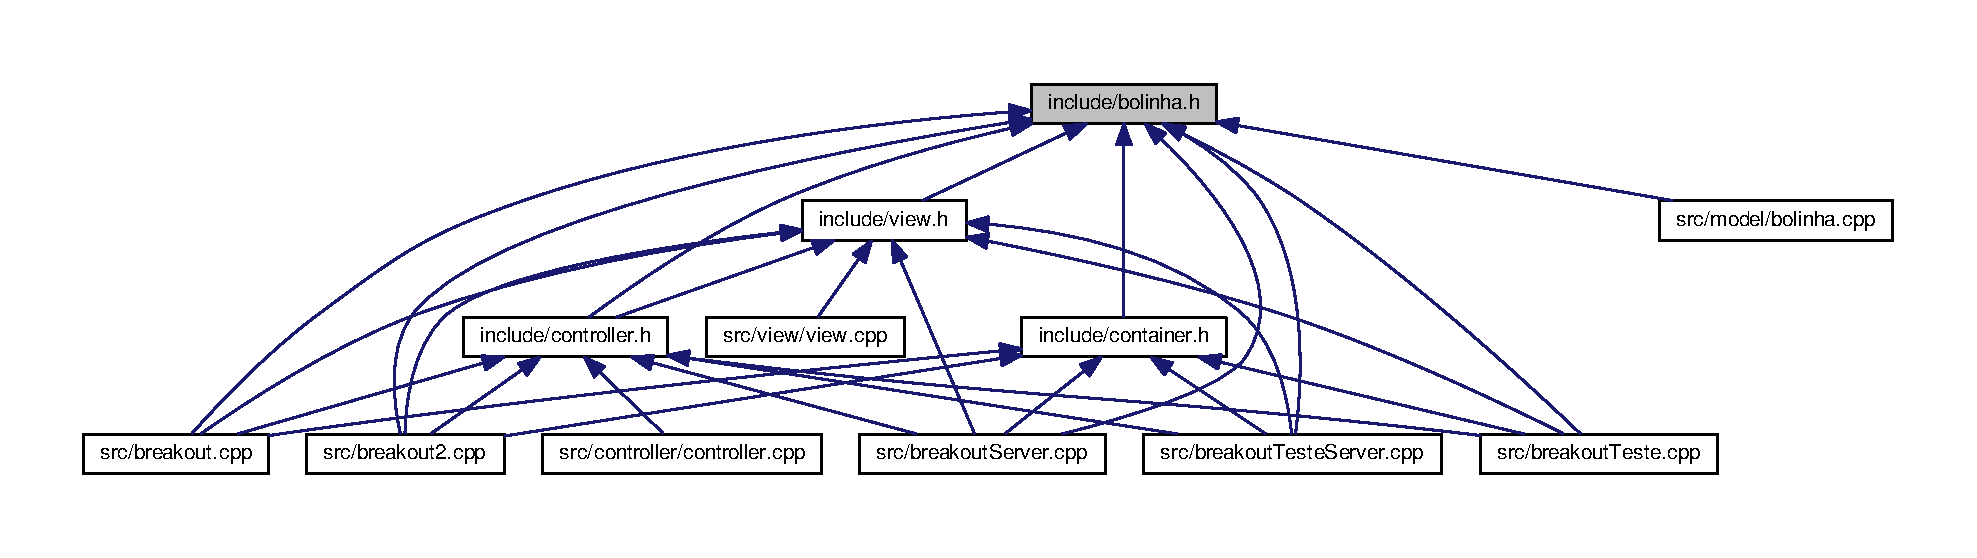
\includegraphics[width=350pt]{bolinha_8h__dep__incl}
\end{center}
\end{figure}
\subsection*{Classes}
\begin{DoxyCompactItemize}
\item 
class \hyperlink{classbolinha}{bolinha}
\begin{DoxyCompactList}\small\item\em Classe para a bolinha. \end{DoxyCompactList}\end{DoxyCompactItemize}

\hypertarget{controller_8h}{}\section{include/controller.h File Reference}
\label{controller_8h}\index{include/controller.\+h@{include/controller.\+h}}
{\ttfamily \#include \char`\"{}barra.\+h\char`\"{}}\\*
{\ttfamily \#include \char`\"{}view.\+h\char`\"{}}\\*
{\ttfamily \#include \char`\"{}bolinha.\+h\char`\"{}}\\*
{\ttfamily \#include \char`\"{}teclado.\+h\char`\"{}}\\*
{\ttfamily \#include $<$S\+D\+L2/\+S\+D\+L.\+h$>$}\\*
Include dependency graph for controller.\+h\+:
\nopagebreak
\begin{figure}[H]
\begin{center}
\leavevmode
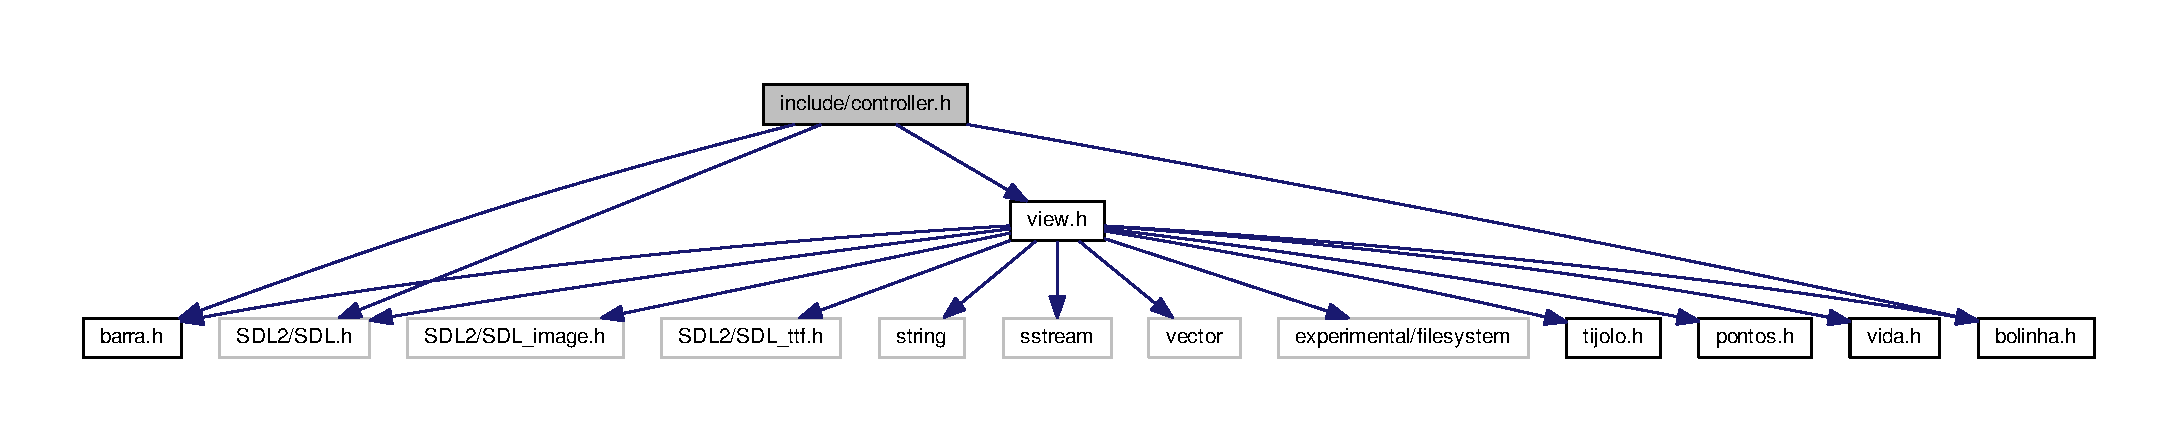
\includegraphics[width=350pt]{controller_8h__incl}
\end{center}
\end{figure}
This graph shows which files directly or indirectly include this file\+:
\nopagebreak
\begin{figure}[H]
\begin{center}
\leavevmode
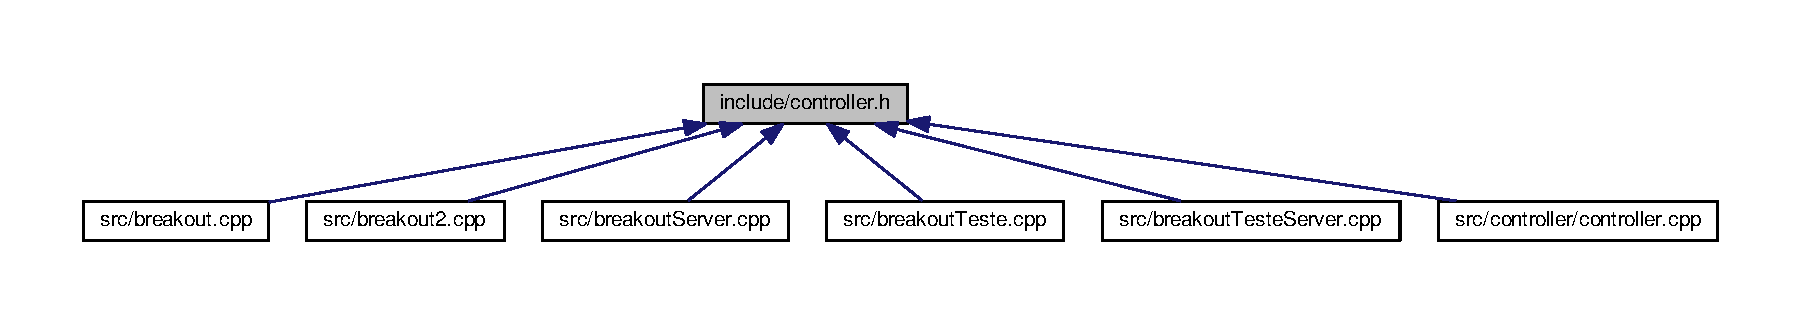
\includegraphics[width=350pt]{controller_8h__dep__incl}
\end{center}
\end{figure}
\subsection*{Classes}
\begin{DoxyCompactItemize}
\item 
class \hyperlink{classcontroller}{controller}
\begin{DoxyCompactList}\small\item\em Classe para o controller. \end{DoxyCompactList}\end{DoxyCompactItemize}

\hypertarget{pontos_8h}{}\section{include/pontos.h File Reference}
\label{pontos_8h}\index{include/pontos.\+h@{include/pontos.\+h}}
{\ttfamily \#include \char`\"{}json.\+hpp\char`\"{}}\\*
Include dependency graph for pontos.\+h\+:
\nopagebreak
\begin{figure}[H]
\begin{center}
\leavevmode
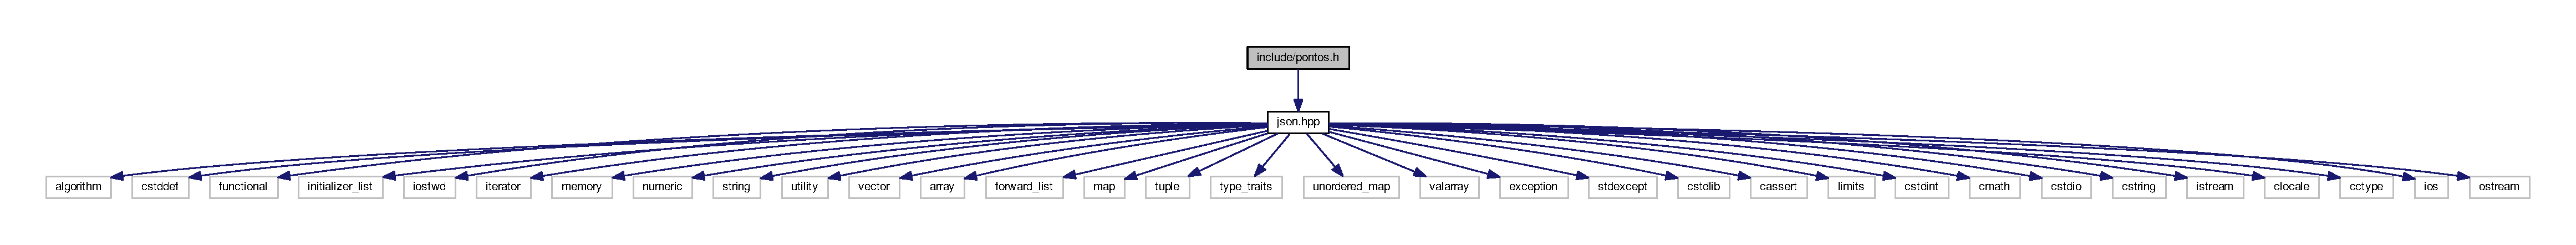
\includegraphics[width=350pt]{pontos_8h__incl}
\end{center}
\end{figure}
This graph shows which files directly or indirectly include this file\+:
\nopagebreak
\begin{figure}[H]
\begin{center}
\leavevmode
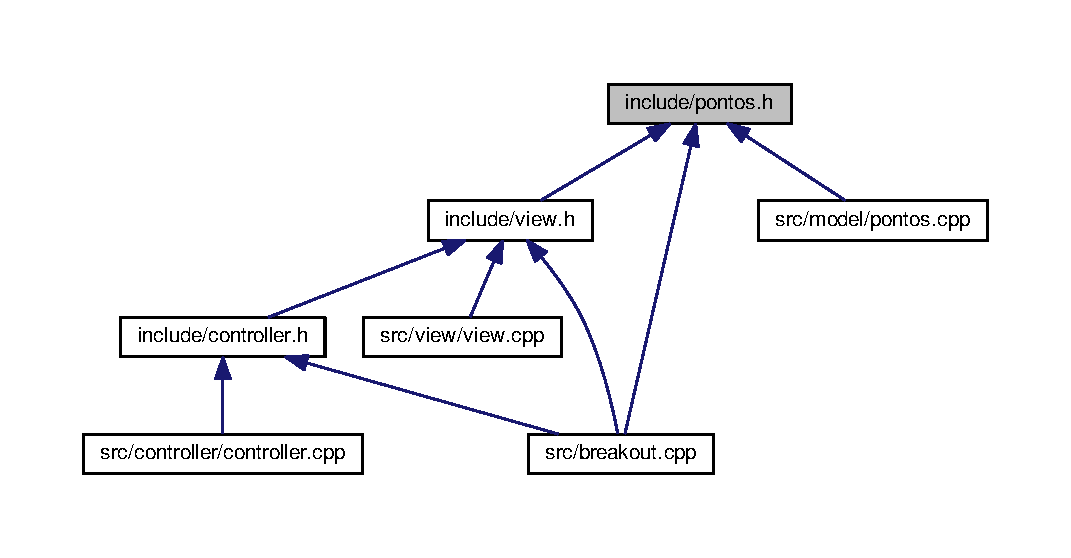
\includegraphics[width=350pt]{pontos_8h__dep__incl}
\end{center}
\end{figure}
\subsection*{Classes}
\begin{DoxyCompactItemize}
\item 
class \hyperlink{classpontos}{pontos}
\begin{DoxyCompactList}\small\item\em Classe para os pontos. \end{DoxyCompactList}\end{DoxyCompactItemize}

\hypertarget{tijolo_8h}{}\section{include/tijolo.h File Reference}
\label{tijolo_8h}\index{include/tijolo.\+h@{include/tijolo.\+h}}
{\ttfamily \#include \char`\"{}json.\+hpp\char`\"{}}\\*
Include dependency graph for tijolo.\+h\+:
\nopagebreak
\begin{figure}[H]
\begin{center}
\leavevmode
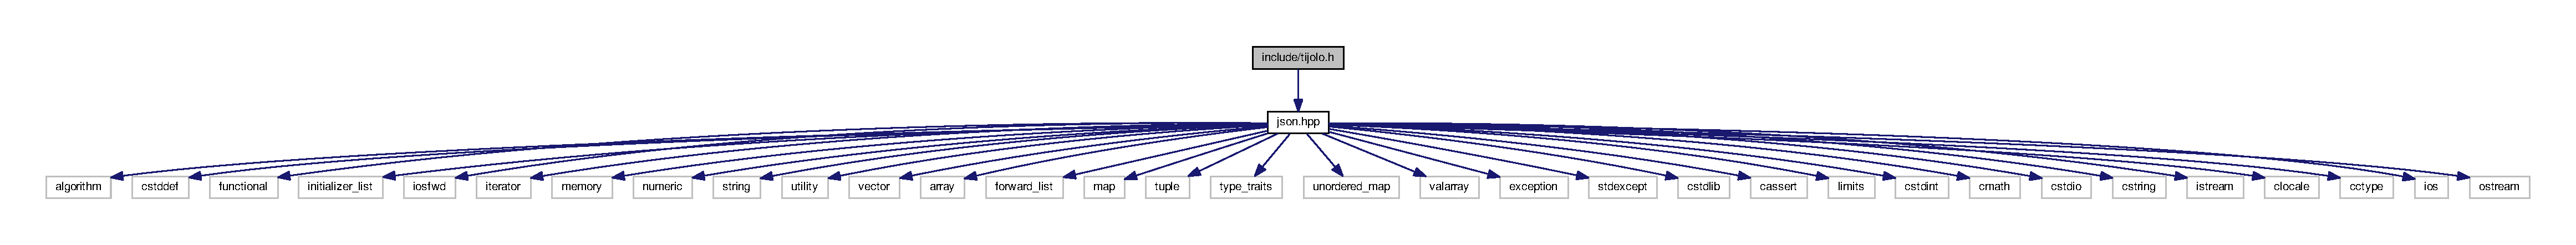
\includegraphics[width=350pt]{tijolo_8h__incl}
\end{center}
\end{figure}
This graph shows which files directly or indirectly include this file\+:
\nopagebreak
\begin{figure}[H]
\begin{center}
\leavevmode
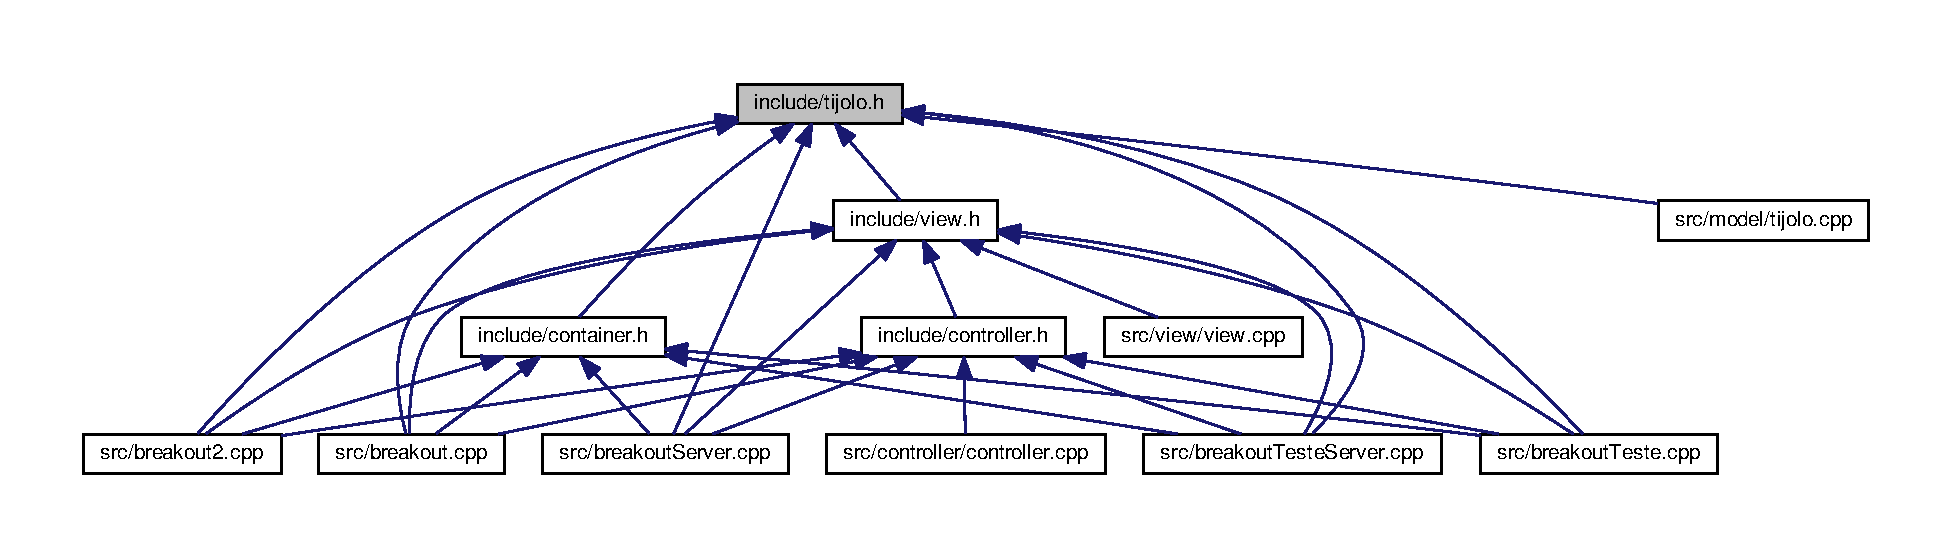
\includegraphics[width=350pt]{tijolo_8h__dep__incl}
\end{center}
\end{figure}
\subsection*{Classes}
\begin{DoxyCompactItemize}
\item 
class \hyperlink{classtijolo}{tijolo}
\begin{DoxyCompactList}\small\item\em Classe para os pontos. \end{DoxyCompactList}\end{DoxyCompactItemize}

\hypertarget{vida_8h}{}\section{include/vida.h File Reference}
\label{vida_8h}\index{include/vida.\+h@{include/vida.\+h}}
This graph shows which files directly or indirectly include this file\+:
\nopagebreak
\begin{figure}[H]
\begin{center}
\leavevmode
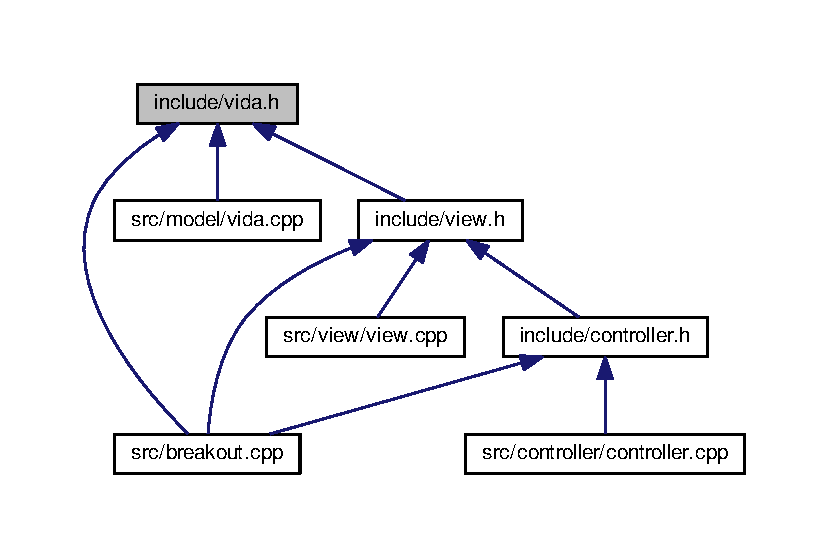
\includegraphics[width=350pt]{vida_8h__dep__incl}
\end{center}
\end{figure}
\subsection*{Classes}
\begin{DoxyCompactItemize}
\item 
class \hyperlink{classvida}{vida}
\begin{DoxyCompactList}\small\item\em Classe para os pontos. \end{DoxyCompactList}\end{DoxyCompactItemize}

\hypertarget{view_8h}{}\section{include/view.h File Reference}
\label{view_8h}\index{include/view.\+h@{include/view.\+h}}
{\ttfamily \#include $<$S\+D\+L2/\+S\+D\+L.\+h$>$}\\*
{\ttfamily \#include $<$S\+D\+L2/\+S\+D\+L\+\_\+image.\+h$>$}\\*
{\ttfamily \#include $<$S\+D\+L2/\+S\+D\+L\+\_\+ttf.\+h$>$}\\*
{\ttfamily \#include $<$string$>$}\\*
{\ttfamily \#include $<$sstream$>$}\\*
{\ttfamily \#include $<$experimental/filesystem$>$}\\*
{\ttfamily \#include \char`\"{}tijolo.\+h\char`\"{}}\\*
{\ttfamily \#include \char`\"{}bolinha.\+h\char`\"{}}\\*
{\ttfamily \#include \char`\"{}barra.\+h\char`\"{}}\\*
{\ttfamily \#include \char`\"{}pontos.\+h\char`\"{}}\\*
{\ttfamily \#include \char`\"{}vida.\+h\char`\"{}}\\*
Include dependency graph for view.\+h\+:\nopagebreak
\begin{figure}[H]
\begin{center}
\leavevmode
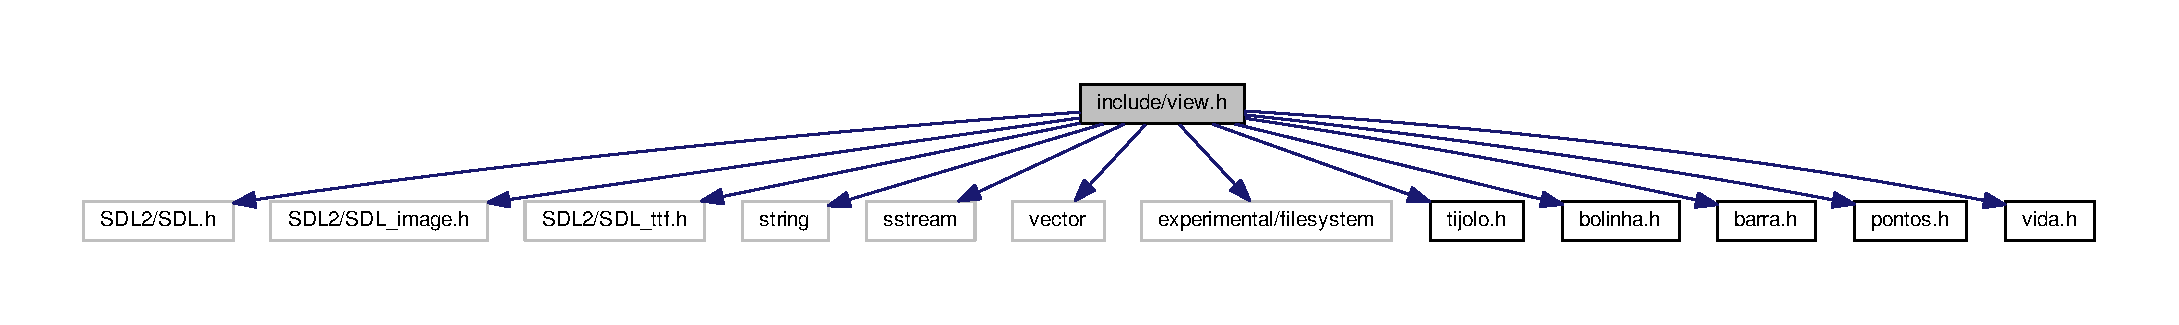
\includegraphics[width=350pt]{view_8h__incl}
\end{center}
\end{figure}
This graph shows which files directly or indirectly include this file\+:\nopagebreak
\begin{figure}[H]
\begin{center}
\leavevmode
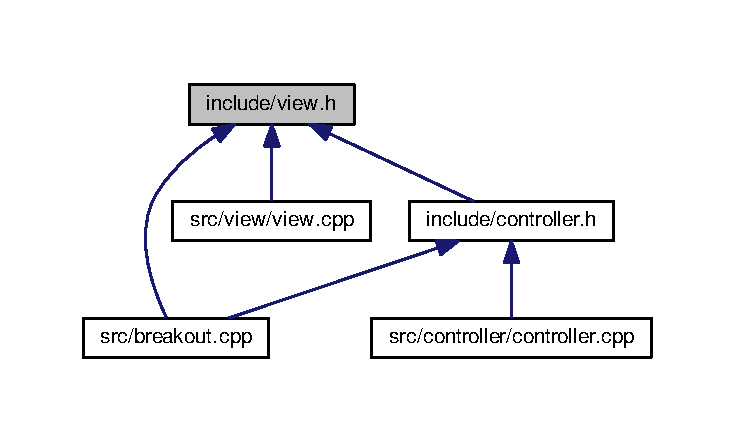
\includegraphics[width=350pt]{view_8h__dep__incl}
\end{center}
\end{figure}
\subsection*{Classes}
\begin{DoxyCompactItemize}
\item 
class \hyperlink{classview}{view}
\begin{DoxyCompactList}\small\item\em Classe para o view. \end{DoxyCompactList}\end{DoxyCompactItemize}

\hypertarget{breakout_8cpp}{}\section{src/breakout.cpp File Reference}
\label{breakout_8cpp}\index{src/breakout.\+cpp@{src/breakout.\+cpp}}
{\ttfamily \#include \char`\"{}view.\+h\char`\"{}}\\*
{\ttfamily \#include \char`\"{}controller.\+h\char`\"{}}\\*
{\ttfamily \#include \char`\"{}tijolo.\+h\char`\"{}}\\*
{\ttfamily \#include \char`\"{}bolinha.\+h\char`\"{}}\\*
{\ttfamily \#include \char`\"{}barra.\+h\char`\"{}}\\*
{\ttfamily \#include \char`\"{}pontos.\+h\char`\"{}}\\*
{\ttfamily \#include \char`\"{}vida.\+h\char`\"{}}\\*
{\ttfamily \#include $<$iostream$>$}\\*
Include dependency graph for breakout.\+cpp\+:
\nopagebreak
\begin{figure}[H]
\begin{center}
\leavevmode
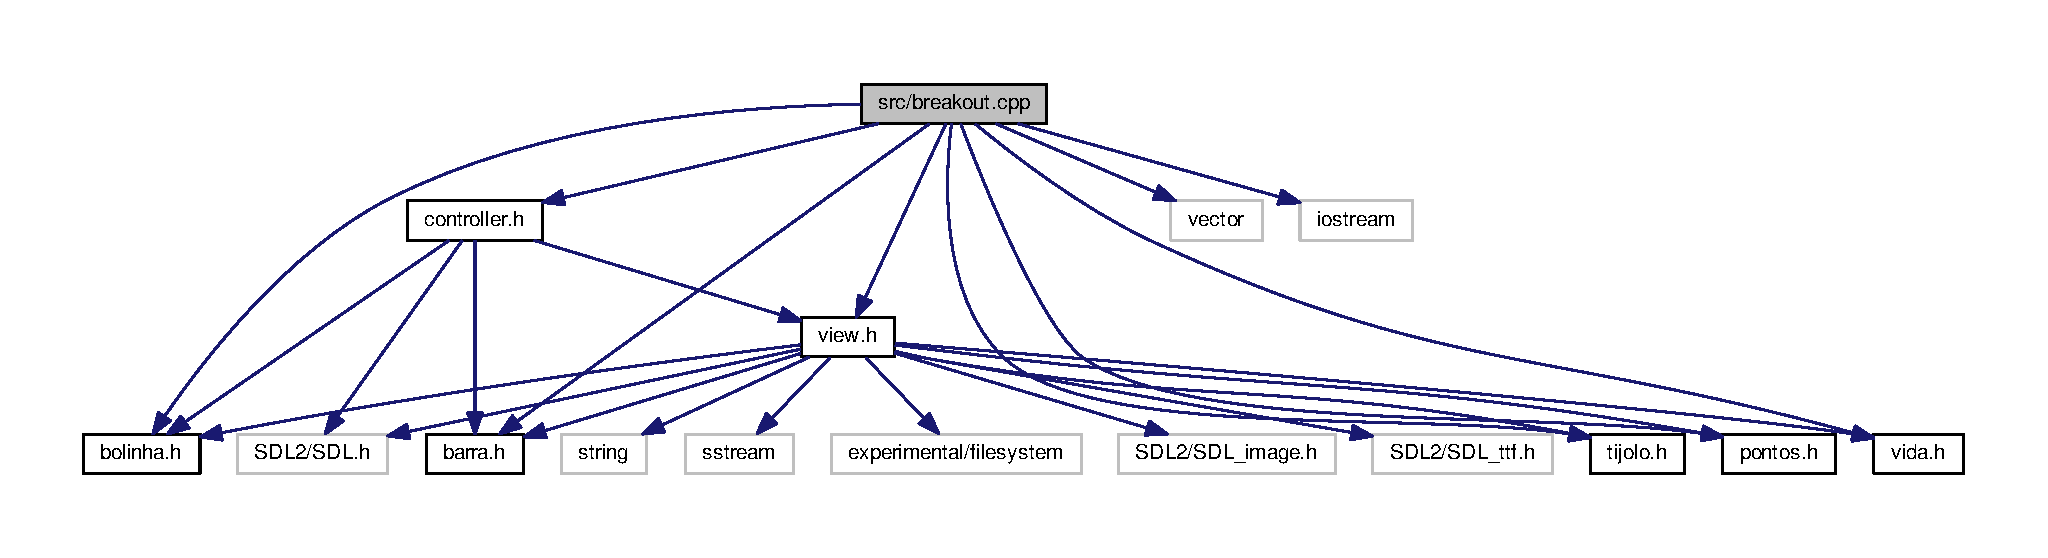
\includegraphics[width=350pt]{breakout_8cpp__incl}
\end{center}
\end{figure}
\subsection*{Functions}
\begin{DoxyCompactItemize}
\item 
int \hyperlink{breakout_8cpp_ae66f6b31b5ad750f1fe042a706a4e3d4}{main} ()
\end{DoxyCompactItemize}


\subsection{Function Documentation}
\index{breakout.\+cpp@{breakout.\+cpp}!main@{main}}
\index{main@{main}!breakout.\+cpp@{breakout.\+cpp}}
\subsubsection[{\texorpdfstring{main()}{main()}}]{\setlength{\rightskip}{0pt plus 5cm}int main (
\begin{DoxyParamCaption}
{}
\end{DoxyParamCaption}
)}\hypertarget{breakout_8cpp_ae66f6b31b5ad750f1fe042a706a4e3d4}{}\label{breakout_8cpp_ae66f6b31b5ad750f1fe042a706a4e3d4}

\hypertarget{controller_8cpp}{}\section{src/controller/controller.cpp File Reference}
\label{controller_8cpp}\index{src/controller/controller.\+cpp@{src/controller/controller.\+cpp}}
{\ttfamily \#include \char`\"{}../../include/controller.\+h\char`\"{}}\\*
{\ttfamily \#include $<$iostream$>$}\\*
Include dependency graph for controller.\+cpp\+:
\nopagebreak
\begin{figure}[H]
\begin{center}
\leavevmode
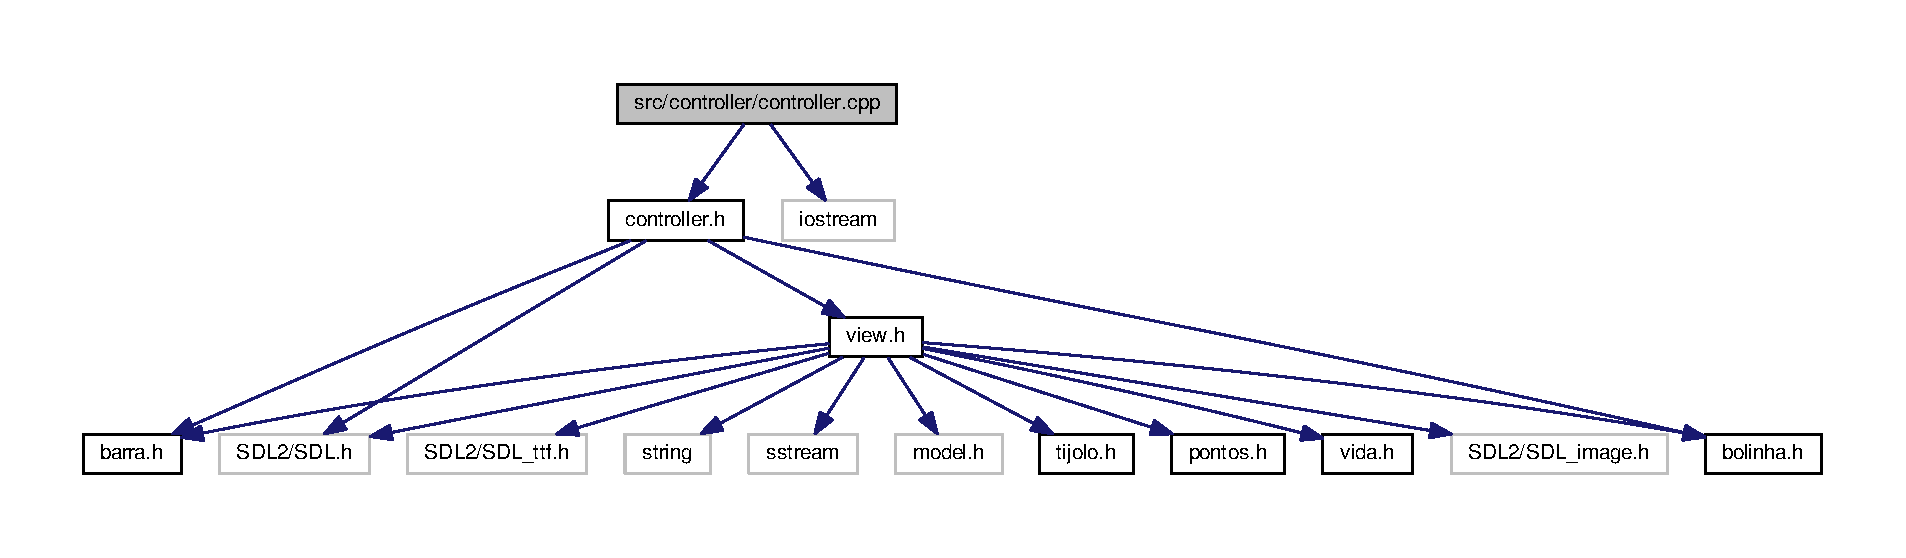
\includegraphics[width=350pt]{controller_8cpp__incl}
\end{center}
\end{figure}

\hypertarget{barra_8cpp}{}\section{src/model/barra.cpp File Reference}
\label{barra_8cpp}\index{src/model/barra.\+cpp@{src/model/barra.\+cpp}}
{\ttfamily \#include \char`\"{}barra.\+h\char`\"{}}\\*
Include dependency graph for barra.\+cpp\+:
\nopagebreak
\begin{figure}[H]
\begin{center}
\leavevmode
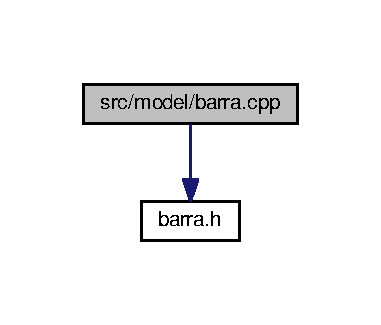
\includegraphics[width=350pt]{barra_8cpp__incl}
\end{center}
\end{figure}

\hypertarget{bolinha_8cpp}{}\section{src/model/bolinha.cpp File Reference}
\label{bolinha_8cpp}\index{src/model/bolinha.\+cpp@{src/model/bolinha.\+cpp}}
{\ttfamily \#include \char`\"{}bolinha.\+h\char`\"{}}\\*
Include dependency graph for bolinha.\+cpp\+:\nopagebreak
\begin{figure}[H]
\begin{center}
\leavevmode
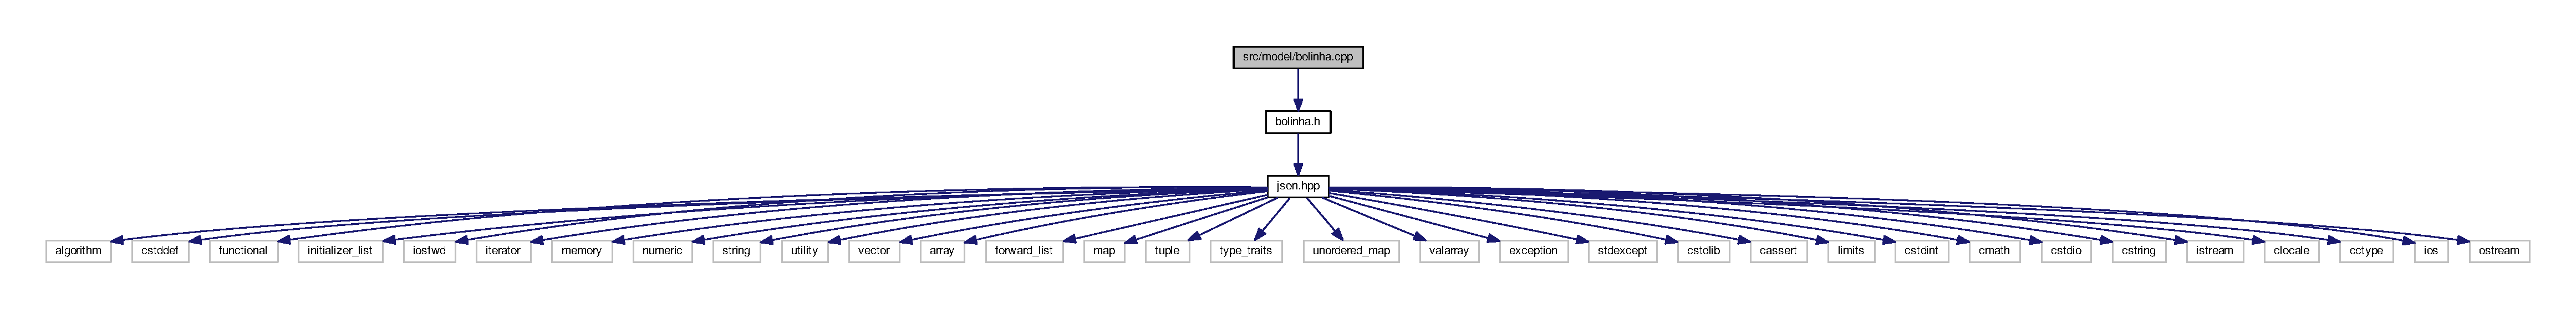
\includegraphics[width=192pt]{bolinha_8cpp__incl}
\end{center}
\end{figure}

\hypertarget{pontos_8cpp}{}\section{src/model/pontos.cpp File Reference}
\label{pontos_8cpp}\index{src/model/pontos.\+cpp@{src/model/pontos.\+cpp}}
{\ttfamily \#include \char`\"{}pontos.\+h\char`\"{}}\\*
Include dependency graph for pontos.\+cpp\+:
\nopagebreak
\begin{figure}[H]
\begin{center}
\leavevmode
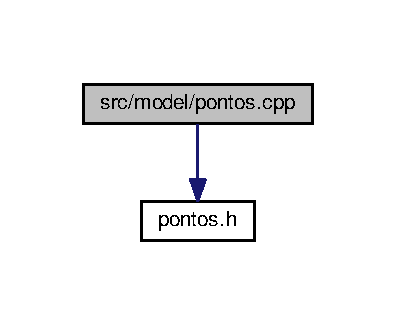
\includegraphics[width=350pt]{pontos_8cpp__incl}
\end{center}
\end{figure}

\hypertarget{tijolo_8cpp}{}\section{src/model/tijolo.cpp File Reference}
\label{tijolo_8cpp}\index{src/model/tijolo.\+cpp@{src/model/tijolo.\+cpp}}
{\ttfamily \#include \char`\"{}tijolo.\+h\char`\"{}}\\*
Include dependency graph for tijolo.\+cpp\+:
\nopagebreak
\begin{figure}[H]
\begin{center}
\leavevmode
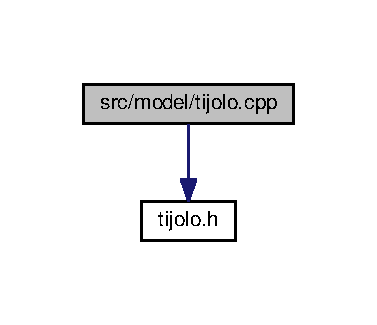
\includegraphics[width=181pt]{tijolo_8cpp__incl}
\end{center}
\end{figure}

\hypertarget{vida_8cpp}{}\section{src/model/vida.cpp File Reference}
\label{vida_8cpp}\index{src/model/vida.\+cpp@{src/model/vida.\+cpp}}
{\ttfamily \#include \char`\"{}vida.\+h\char`\"{}}\\*
Include dependency graph for vida.\+cpp\+:
\nopagebreak
\begin{figure}[H]
\begin{center}
\leavevmode
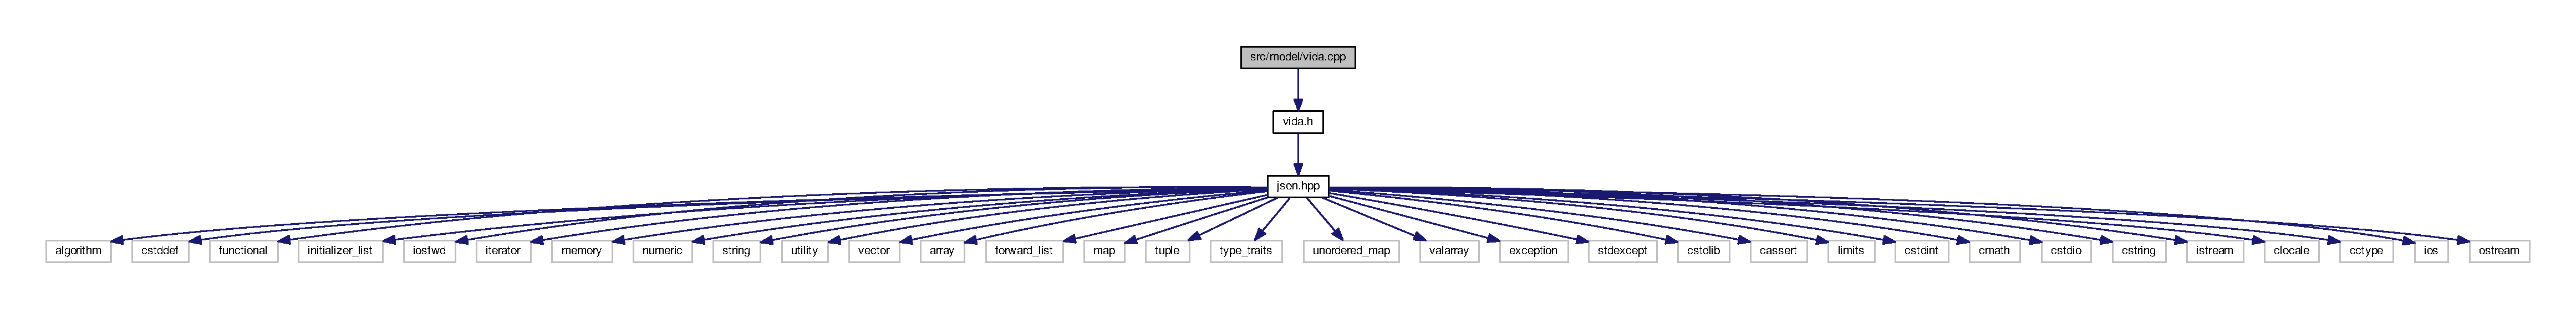
\includegraphics[width=179pt]{vida_8cpp__incl}
\end{center}
\end{figure}

\hypertarget{view_8cpp}{}\section{src/view/view.cpp File Reference}
\label{view_8cpp}\index{src/view/view.\+cpp@{src/view/view.\+cpp}}
{\ttfamily \#include \char`\"{}view.\+h\char`\"{}}\\*
{\ttfamily \#include $<$iostream$>$}\\*
{\ttfamily \#include $<$string$>$}\\*
{\ttfamily \#include $<$experimental/filesystem$>$}\\*
{\ttfamily \#include $<$unistd.\+h$>$}\\*
Include dependency graph for view.\+cpp\+:\nopagebreak
\begin{figure}[H]
\begin{center}
\leavevmode
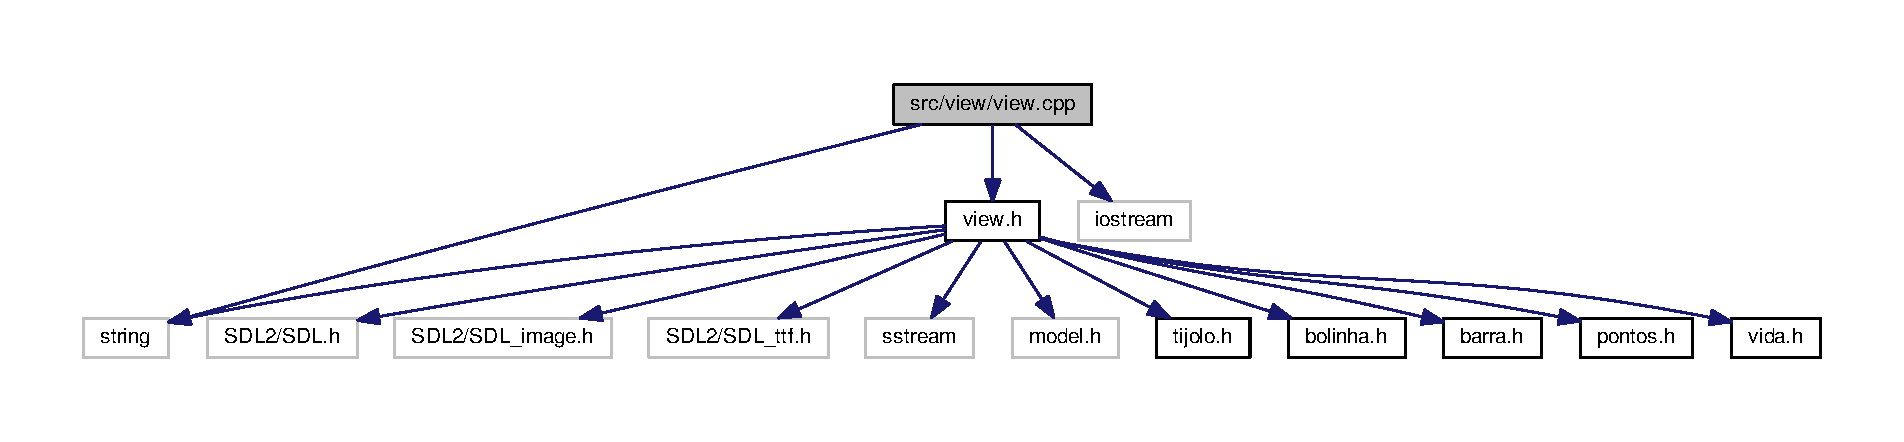
\includegraphics[width=350pt]{view_8cpp__incl}
\end{center}
\end{figure}
\subsection*{Variables}
\begin{DoxyCompactItemize}
\item 
int \hyperlink{view_8cpp_a599adbe412c60e0cc5abb86be7ee4507}{S\+C\+R\+E\+E\+N\+\_\+\+W\+I\+D\+TH} = 720
\item 
int \hyperlink{view_8cpp_af1c710caf1e3a9e81829078054e83799}{S\+C\+R\+E\+E\+N\+\_\+\+H\+E\+I\+G\+HT} = 480
\item 
S\+D\+L\+\_\+\+Color \hyperlink{view_8cpp_afd2fcdbc10ee4f7ed94f8f0d27ee44ed}{White} = \{255, 255, 255\}
\item 
S\+D\+L\+\_\+\+Color \hyperlink{view_8cpp_abe117c50d0fa5c3cecfdc127234f5093}{Red} = \{255, 0, 0\}
\item 
S\+D\+L\+\_\+\+Color \hyperlink{view_8cpp_a3ce40599515f4a263a05fb8e176d89e3}{Green} = \{0, 255, 0\}
\item 
char \hyperlink{view_8cpp_aba7b55804629711727b7b1176c7583aa}{num\+\_\+char} \mbox{[}10+sizeof(char)\mbox{]}
\item 
char \hyperlink{view_8cpp_a5c164fe165bdff98f887ade2436b7f06}{tmp} \mbox{[}256\mbox{]}
\end{DoxyCompactItemize}


\subsection{Variable Documentation}
\index{view.\+cpp@{view.\+cpp}!Green@{Green}}
\index{Green@{Green}!view.\+cpp@{view.\+cpp}}
\subsubsection[{\texorpdfstring{Green}{Green}}]{\setlength{\rightskip}{0pt plus 5cm}S\+D\+L\+\_\+\+Color Green = \{0, 255, 0\}}\hypertarget{view_8cpp_a3ce40599515f4a263a05fb8e176d89e3}{}\label{view_8cpp_a3ce40599515f4a263a05fb8e176d89e3}
\index{view.\+cpp@{view.\+cpp}!num\+\_\+char@{num\+\_\+char}}
\index{num\+\_\+char@{num\+\_\+char}!view.\+cpp@{view.\+cpp}}
\subsubsection[{\texorpdfstring{num\+\_\+char}{num_char}}]{\setlength{\rightskip}{0pt plus 5cm}char num\+\_\+char\mbox{[}10+sizeof(char)\mbox{]}}\hypertarget{view_8cpp_aba7b55804629711727b7b1176c7583aa}{}\label{view_8cpp_aba7b55804629711727b7b1176c7583aa}
\index{view.\+cpp@{view.\+cpp}!Red@{Red}}
\index{Red@{Red}!view.\+cpp@{view.\+cpp}}
\subsubsection[{\texorpdfstring{Red}{Red}}]{\setlength{\rightskip}{0pt plus 5cm}S\+D\+L\+\_\+\+Color Red = \{255, 0, 0\}}\hypertarget{view_8cpp_abe117c50d0fa5c3cecfdc127234f5093}{}\label{view_8cpp_abe117c50d0fa5c3cecfdc127234f5093}
\index{view.\+cpp@{view.\+cpp}!S\+C\+R\+E\+E\+N\+\_\+\+H\+E\+I\+G\+HT@{S\+C\+R\+E\+E\+N\+\_\+\+H\+E\+I\+G\+HT}}
\index{S\+C\+R\+E\+E\+N\+\_\+\+H\+E\+I\+G\+HT@{S\+C\+R\+E\+E\+N\+\_\+\+H\+E\+I\+G\+HT}!view.\+cpp@{view.\+cpp}}
\subsubsection[{\texorpdfstring{S\+C\+R\+E\+E\+N\+\_\+\+H\+E\+I\+G\+HT}{SCREEN_HEIGHT}}]{\setlength{\rightskip}{0pt plus 5cm}int S\+C\+R\+E\+E\+N\+\_\+\+H\+E\+I\+G\+HT = 480}\hypertarget{view_8cpp_af1c710caf1e3a9e81829078054e83799}{}\label{view_8cpp_af1c710caf1e3a9e81829078054e83799}
\index{view.\+cpp@{view.\+cpp}!S\+C\+R\+E\+E\+N\+\_\+\+W\+I\+D\+TH@{S\+C\+R\+E\+E\+N\+\_\+\+W\+I\+D\+TH}}
\index{S\+C\+R\+E\+E\+N\+\_\+\+W\+I\+D\+TH@{S\+C\+R\+E\+E\+N\+\_\+\+W\+I\+D\+TH}!view.\+cpp@{view.\+cpp}}
\subsubsection[{\texorpdfstring{S\+C\+R\+E\+E\+N\+\_\+\+W\+I\+D\+TH}{SCREEN_WIDTH}}]{\setlength{\rightskip}{0pt plus 5cm}int S\+C\+R\+E\+E\+N\+\_\+\+W\+I\+D\+TH = 720}\hypertarget{view_8cpp_a599adbe412c60e0cc5abb86be7ee4507}{}\label{view_8cpp_a599adbe412c60e0cc5abb86be7ee4507}
\index{view.\+cpp@{view.\+cpp}!tmp@{tmp}}
\index{tmp@{tmp}!view.\+cpp@{view.\+cpp}}
\subsubsection[{\texorpdfstring{tmp}{tmp}}]{\setlength{\rightskip}{0pt plus 5cm}char tmp\mbox{[}256\mbox{]}}\hypertarget{view_8cpp_a5c164fe165bdff98f887ade2436b7f06}{}\label{view_8cpp_a5c164fe165bdff98f887ade2436b7f06}
\index{view.\+cpp@{view.\+cpp}!White@{White}}
\index{White@{White}!view.\+cpp@{view.\+cpp}}
\subsubsection[{\texorpdfstring{White}{White}}]{\setlength{\rightskip}{0pt plus 5cm}S\+D\+L\+\_\+\+Color White = \{255, 255, 255\}}\hypertarget{view_8cpp_afd2fcdbc10ee4f7ed94f8f0d27ee44ed}{}\label{view_8cpp_afd2fcdbc10ee4f7ed94f8f0d27ee44ed}

%--- End generated contents ---

% Index
\backmatter
\newpage
\phantomsection
\clearemptydoublepage
\addcontentsline{toc}{chapter}{Index}
\printindex

\end{document}
